% reducesymm/QFT/correspnd.tex
% $Author$ $Date$
% Predrag  switched to github.com               jul  8 2013

\section{Is QED finite? Correspondence}
\label{sect:correspnd}


\begin{bartlett}{
I am not sure I'll will tell you anything useful any time soon, as I'm a
lapsed field theorist, but here is for your amusement my
\HREF{https://vimeo.com/79605418} {recent rant}. To
cite my wife: ``You may well be right".
        }
\bauthor{
\HREF{http://www.goodreads.com/work/quotes/3226250-keep-the-aspidistra-flying}
{Keep the Aspidistra Flying!}
    }
\end{bartlett}
\bigskip



\begin{description}

\item[2007-03-18 Dirk Kreimer] % kreimer@ihes.fr via nbi.dk
I was pretty much looking forward to grab you for a chat on Dyson
Schwinger etc whilst in Bonn this starting week. Now I fail to be there
myself due to a stupid mechanical problem with a vertebrae.
Pondering about other options, let me just point out that the IHES
(www.ihes.fr) has an excellent visitor program. If you foresee some time
you fancy to pay us a visit, please go ahead.

I am running a little seminar at Boston whilst being there, so besides
what works out with IHES,  whenever you are available in the above
period, you are herewith invited for a talk at BU.
Would you be able to come for a seminar to Boston, Thu, Nov 29 this year?

\item[2011-08-23 Predrag] to Dirk:

I feel like some stuck-up god knows who for not having answered sooner -
but it is not that. I have been focusing on turbulence (with the goal of
using what I learn on Yang-Mills, eventually - if it works, Feynman
diagrammar will be of secondary importance, the first step is fully and
totally non-perturbative) so I feel like fraud talking about QFT when I
am suspended between the perturbative past and the elusive
non-perturbative future.

If someone wants to hear about turbulence as in
\HREF{http://ChaosBook.org/tutorials} {ChaosBook.org/tutorials}, I can do
that honestly - otherwise we wait until I actually do any QFT worth
hearing about...

I got \HREF{http://birdtracks.eu} {birdtracks.eu} published, finally -
you get 100 birdtracks per 1\$, a real deal if you are into that kind of
thing.

Guilty as Charged -
Predrag

\item[2011-08-26 Dirk]
June 01-05 2009 I am organizing a workshop at IHES. It has a
non-perturbative component via Dyson--Schwinger eqs. Would you be
interested to participate and come?

\item[2017-06-16 Dirk]
I will show your notes to
Henry Ki{\ss}ler\rf{Kissler16}   <kissler@physik.hu-berlin.de>
and
\HREF{http://people.physik.hu-berlin.de/~borinsky/}
{Michael Borinsky}\rf{Borinsky14,Borinsky17}    <borinsky@physik.hu-berlin.de> .

There should be a few people at Les Houches June 2018 who have something
to say about asymptotics of solutions of Dyson-Schwinger equation for
example.


\end{description}

%% Laporta17figuragau.tex %%%%%
%% compiled by  reducesymm/QFT/blog.tex
%%%%%%%%%%%%%%%%%%%%%%%%%%%%%%%%%%%%%%%%
\begin{figure}
\begin{center}
\begin{picture}(125,325)(70,50)
\thicklines
%%%
{
\put(+000.0,+200.0){\makebox(0,0)[lb]{
% fotone obliquo (0.000000,200.000000) (0.000000,205.000000)
   \qbezier(+000.0,+200.0)(+001.2,+201.2)(+000.0,+202.5)
   \qbezier(+000.0,+202.5)(-001.2,+203.8)(+000.0,+205.0)
% elettrone curvo (0.000000,200.000000) (-20.000000,160.000000) 1000.000000
% cerchio r=44721.365140 c=(-40010.000000,20180.000000) ang=(-26.536403,-26.593699)
   \qbezier(+000.0,+200.0)(-010.0,+180.0)(-020.0,+160.0)
% elettrone curvo (0.000000,200.000000) (20.000000,160.000000) 1000.000000
% cerchio r=44721.365140 c=(-39990.000000,-19820.000000) ang=(26.593699,26.536403)
   \qbezier(+000.0,+200.0)(+010.0,+180.0)(+020.0,+160.0)
% fotone obliquo (-14.142136,171.715729) (14.142136,171.715729)
   \qbezier(-014.1,+171.7)(-013.3,+170.8)(-012.4,+171.7)
   \qbezier(-012.4,+171.7)(-011.5,+172.6)(-010.6,+171.7)
   \qbezier(-010.6,+171.7)(-009.7,+170.8)(-008.8,+171.7)
   \qbezier(-008.8,+171.7)(-008.0,+172.6)(-007.1,+171.7)
   \qbezier(-007.1,+171.7)(-006.2,+170.8)(-005.3,+171.7)
   \qbezier(-005.3,+171.7)(-004.4,+172.6)(-003.5,+171.7)
   \qbezier(-003.5,+171.7)(-002.7,+170.8)(-001.8,+171.7)
   \qbezier(-001.8,+171.7)(-000.9,+172.6)(+000.0,+171.7)
   \qbezier(+000.0,+171.7)(+000.9,+170.8)(+001.8,+171.7)
   \qbezier(+001.8,+171.7)(+002.7,+172.6)(+003.5,+171.7)
   \qbezier(+003.5,+171.7)(+004.4,+170.8)(+005.3,+171.7)
   \qbezier(+005.3,+171.7)(+006.2,+172.6)(+007.1,+171.7)
   \qbezier(+007.1,+171.7)(+008.0,+170.8)(+008.8,+171.7)
   \qbezier(+008.8,+171.7)(+009.7,+172.6)(+010.6,+171.7)
   \qbezier(+010.6,+171.7)(+011.5,+170.8)(+012.4,+171.7)
   \qbezier(+012.4,+171.7)(+013.3,+172.6)(+014.1,+171.7)
% fotone curvo (5.303301,189.393398) (10.000000,180.000000) 0.100000
% fotone semicircolare r=5.355061 c=(6.712311,184.227029) ang=(105.255119,-52.125016)
% n=8
   \qbezier(+005.3,+189.4)(+006.3,+188.7)(+007.1,+189.6)
   \qbezier(+007.1,+189.6)(+008.3,+190.3)(+008.9,+189.1)
   \qbezier(+008.9,+189.1)(+009.2,+187.9)(+010.4,+188.1)
   \qbezier(+010.4,+188.1)(+011.7,+187.9)(+011.5,+186.6)
   \qbezier(+011.5,+186.6)(+011.0,+185.5)(+012.0,+184.9)
   \qbezier(+012.0,+184.9)(+013.0,+183.9)(+011.9,+183.0)
   \qbezier(+011.9,+183.0)(+010.8,+182.5)(+011.2,+181.4)
   \qbezier(+011.2,+181.4)(+011.3,+180.0)(+010.0,+180.0)
% fotone curvo (12.247449,175.505103) (17.320508,165.358984) 0.100000
% fotone semicircolare r=5.784178 c=(13.769367,169.924737) ang=(105.255119,-52.125016)
% n=9
   \qbezier(+012.2,+175.5)(+013.2,+174.8)(+014.0,+175.7)
   \qbezier(+014.0,+175.7)(+015.0,+176.5)(+015.7,+175.4)
   \qbezier(+015.7,+175.4)(+016.1,+174.2)(+017.3,+174.5)
   \qbezier(+017.3,+174.5)(+018.6,+174.6)(+018.5,+173.3)
   \qbezier(+018.5,+173.3)(+018.2,+172.1)(+019.3,+171.7)
   \qbezier(+019.3,+171.7)(+020.3,+171.0)(+019.6,+170.0)
   \qbezier(+019.6,+170.0)(+018.6,+169.2)(+019.3,+168.2)
   \qbezier(+019.3,+168.2)(+019.8,+167.0)(+018.5,+166.6)
   \qbezier(+018.5,+166.6)(+017.3,+166.5)(+017.3,+165.4)
% fotone curvo (15.811388,168.377223) (18.708287,162.583426) -0.100000
% fotone semicircolare r=3.302973 c=(17.839217,165.770015) ang=(127.874984,285.255119)
% n=5
   \qbezier(+015.8,+168.4)(+014.5,+168.2)(+014.7,+166.9)
   \qbezier(+014.7,+166.9)(+015.4,+166.0)(+014.6,+165.1)
   \qbezier(+014.6,+165.1)(+014.1,+163.9)(+015.4,+163.5)
   \qbezier(+015.4,+163.5)(+016.5,+163.7)(+016.9,+162.6)
   \qbezier(+016.9,+162.6)(+017.8,+161.6)(+018.7,+162.6)
\put(+000.0,+152.0){\makebox(0,0){$(1)$}}
}}
\put(+025.0,+200.0){\makebox(0,0)[lb]{
% fotone obliquo (25.000000,200.000000) (25.000000,205.000000)
   \qbezier(+025.0,+200.0)(+026.2,+201.2)(+025.0,+202.5)
   \qbezier(+025.0,+202.5)(+023.8,+203.8)(+025.0,+205.0)
% elettrone curvo (25.000000,200.000000) (5.000000,160.000000) 1000.000000
% cerchio r=44721.365140 c=(-39985.000000,20180.000000) ang=(-26.536403,-26.593699)
   \qbezier(+025.0,+200.0)(+015.0,+180.0)(+005.0,+160.0)
% elettrone curvo (25.000000,200.000000) (45.000000,160.000000) 1000.000000
% cerchio r=44721.365140 c=(-39965.000000,-19820.000000) ang=(26.593699,26.536403)
   \qbezier(+025.0,+200.0)(+035.0,+180.0)(+045.0,+160.0)
% fotone obliquo (14.309550,178.619101) (35.690450,178.619101)
   \qbezier(+014.3,+178.6)(+015.2,+177.7)(+016.1,+178.6)
   \qbezier(+016.1,+178.6)(+017.0,+179.5)(+017.9,+178.6)
   \qbezier(+017.9,+178.6)(+018.8,+177.7)(+019.7,+178.6)
   \qbezier(+019.7,+178.6)(+020.5,+179.5)(+021.4,+178.6)
   \qbezier(+021.4,+178.6)(+022.3,+177.7)(+023.2,+178.6)
   \qbezier(+023.2,+178.6)(+024.1,+179.5)(+025.0,+178.6)
   \qbezier(+025.0,+178.6)(+025.9,+177.7)(+026.8,+178.6)
   \qbezier(+026.8,+178.6)(+027.7,+179.5)(+028.6,+178.6)
   \qbezier(+028.6,+178.6)(+029.5,+177.7)(+030.3,+178.6)
   \qbezier(+030.3,+178.6)(+031.2,+179.5)(+032.1,+178.6)
   \qbezier(+032.1,+178.6)(+033.0,+177.7)(+033.9,+178.6)
   \qbezier(+033.9,+178.6)(+034.8,+179.5)(+035.7,+178.6)
% fotone obliquo (8.096915,166.193830) (41.903085,166.193830)
   \qbezier(+008.1,+166.2)(+009.0,+165.3)(+009.9,+166.2)
   \qbezier(+009.9,+166.2)(+010.8,+167.1)(+011.7,+166.2)
   \qbezier(+011.7,+166.2)(+012.5,+165.3)(+013.4,+166.2)
   \qbezier(+013.4,+166.2)(+014.3,+167.1)(+015.2,+166.2)
   \qbezier(+015.2,+166.2)(+016.1,+165.3)(+017.0,+166.2)
   \qbezier(+017.0,+166.2)(+017.9,+167.1)(+018.8,+166.2)
   \qbezier(+018.8,+166.2)(+019.7,+165.3)(+020.6,+166.2)
   \qbezier(+020.6,+166.2)(+021.4,+167.1)(+022.3,+166.2)
   \qbezier(+022.3,+166.2)(+023.2,+165.3)(+024.1,+166.2)
   \qbezier(+024.1,+166.2)(+025.0,+167.1)(+025.9,+166.2)
   \qbezier(+025.9,+166.2)(+026.8,+165.3)(+027.7,+166.2)
   \qbezier(+027.7,+166.2)(+028.6,+167.1)(+029.4,+166.2)
   \qbezier(+029.4,+166.2)(+030.3,+165.3)(+031.2,+166.2)
   \qbezier(+031.2,+166.2)(+032.1,+167.1)(+033.0,+166.2)
   \qbezier(+033.0,+166.2)(+033.9,+165.3)(+034.8,+166.2)
   \qbezier(+034.8,+166.2)(+035.7,+167.1)(+036.6,+166.2)
   \qbezier(+036.6,+166.2)(+037.5,+165.3)(+038.3,+166.2)
   \qbezier(+038.3,+166.2)(+039.2,+167.1)(+040.1,+166.2)
   \qbezier(+040.1,+166.2)(+041.0,+165.3)(+041.9,+166.2)
% fotone curvo (32.559289,184.881421) (38.093073,173.813853) 0.100000
% fotone semicircolare r=6.309484 c=(34.219425,178.794259) ang=(105.255119,-52.125016)
% n=9
   \qbezier(+032.6,+184.9)(+033.6,+184.1)(+034.5,+185.1)
   \qbezier(+034.5,+185.1)(+035.6,+185.9)(+036.3,+184.7)
   \qbezier(+036.3,+184.7)(+036.8,+183.5)(+038.0,+183.8)
   \qbezier(+038.0,+183.8)(+039.4,+183.8)(+039.4,+182.4)
   \qbezier(+039.4,+182.4)(+039.0,+181.2)(+040.2,+180.7)
   \qbezier(+040.2,+180.7)(+041.4,+179.9)(+040.5,+178.8)
   \qbezier(+040.5,+178.8)(+039.5,+178.0)(+040.2,+176.9)
   \qbezier(+040.2,+176.9)(+040.7,+175.6)(+039.4,+175.2)
   \qbezier(+039.4,+175.2)(+038.1,+175.1)(+038.1,+173.8)
% fotone curvo (40.118579,169.762842) (43.516402,162.967196) 0.100000
% fotone semicircolare r=3.874114 c=(41.137926,166.025237) ang=(105.255119,-52.125016)
% n=6
   \qbezier(+040.1,+169.8)(+041.0,+169.0)(+041.9,+169.8)
   \qbezier(+041.9,+169.8)(+043.1,+170.3)(+043.5,+169.1)
   \qbezier(+043.5,+169.1)(+043.5,+168.0)(+044.6,+167.8)
   \qbezier(+044.6,+167.8)(+045.7,+167.1)(+045.0,+166.0)
   \qbezier(+045.0,+166.0)(+044.1,+165.4)(+044.6,+164.3)
   \qbezier(+044.6,+164.3)(+044.8,+163.0)(+043.5,+163.0)
\put(+025.0,+152.0){\makebox(0,0){$(2)$}}
}}
\put(+050.0,+200.0){\makebox(0,0)[lb]{
% fotone obliquo (50.000000,200.000000) (50.000000,205.000000)
   \qbezier(+050.0,+200.0)(+051.2,+201.2)(+050.0,+202.5)
   \qbezier(+050.0,+202.5)(+048.8,+203.8)(+050.0,+205.0)
% elettrone curvo (50.000000,200.000000) (30.000000,160.000000) 1000.000000
% cerchio r=44721.365140 c=(-39960.000000,20180.000000) ang=(-26.536403,-26.593699)
   \qbezier(+050.0,+200.0)(+040.0,+180.0)(+030.0,+160.0)
% elettrone curvo (50.000000,200.000000) (70.000000,160.000000) 1000.000000
% cerchio r=44721.365140 c=(-39940.000000,-19820.000000) ang=(26.593699,26.536403)
   \qbezier(+050.0,+200.0)(+060.0,+180.0)(+070.0,+160.0)
% fotone obliquo (33.670068,167.340137) (66.329932,167.340137)
   \qbezier(+033.7,+167.3)(+034.5,+166.5)(+035.4,+167.3)
   \qbezier(+035.4,+167.3)(+036.2,+168.2)(+037.1,+167.3)
   \qbezier(+037.1,+167.3)(+038.0,+166.5)(+038.8,+167.3)
   \qbezier(+038.8,+167.3)(+039.7,+168.2)(+040.5,+167.3)
   \qbezier(+040.5,+167.3)(+041.4,+166.5)(+042.3,+167.3)
   \qbezier(+042.3,+167.3)(+043.1,+168.2)(+044.0,+167.3)
   \qbezier(+044.0,+167.3)(+044.8,+166.5)(+045.7,+167.3)
   \qbezier(+045.7,+167.3)(+046.6,+168.2)(+047.4,+167.3)
   \qbezier(+047.4,+167.3)(+048.3,+166.5)(+049.1,+167.3)
   \qbezier(+049.1,+167.3)(+050.0,+168.2)(+050.9,+167.3)
   \qbezier(+050.9,+167.3)(+051.7,+166.5)(+052.6,+167.3)
   \qbezier(+052.6,+167.3)(+053.4,+168.2)(+054.3,+167.3)
   \qbezier(+054.3,+167.3)(+055.2,+166.5)(+056.0,+167.3)
   \qbezier(+056.0,+167.3)(+056.9,+168.2)(+057.7,+167.3)
   \qbezier(+057.7,+167.3)(+058.6,+166.5)(+059.5,+167.3)
   \qbezier(+059.5,+167.3)(+060.3,+168.2)(+061.2,+167.3)
   \qbezier(+061.2,+167.3)(+062.0,+166.5)(+062.9,+167.3)
   \qbezier(+062.9,+167.3)(+063.8,+168.2)(+064.6,+167.3)
   \qbezier(+064.6,+167.3)(+065.5,+166.5)(+066.3,+167.3)
% fotone curvo (35.857864,171.715729) (31.742581,163.485163) -0.100000
% fotone semicircolare r=4.692144 c=(34.623279,167.188917) ang=(74.744881,232.125016)
% n=7
   \qbezier(+035.9,+171.7)(+035.0,+172.8)(+034.0,+171.8)
   \qbezier(+034.0,+171.8)(+033.4,+170.8)(+032.3,+171.3)
   \qbezier(+032.3,+171.3)(+031.0,+171.4)(+030.9,+170.1)
   \qbezier(+030.9,+170.1)(+031.2,+168.9)(+030.1,+168.4)
   \qbezier(+030.1,+168.4)(+029.0,+167.6)(+030.0,+166.6)
   \qbezier(+030.0,+166.6)(+031.0,+166.0)(+030.5,+164.9)
   \qbezier(+030.5,+164.9)(+030.4,+163.5)(+031.7,+163.5)
% fotone curvo (64.142136,171.715729) (68.257419,163.485163) 0.100000
% fotone semicircolare r=4.692144 c=(65.376721,167.188917) ang=(105.255119,-52.125016)
% n=7
   \qbezier(+064.1,+171.7)(+065.1,+171.0)(+066.0,+171.8)
   \qbezier(+066.0,+171.8)(+067.1,+172.5)(+067.7,+171.3)
   \qbezier(+067.7,+171.3)(+067.9,+170.1)(+069.1,+170.1)
   \qbezier(+069.1,+170.1)(+070.4,+169.7)(+069.9,+168.4)
   \qbezier(+069.9,+168.4)(+069.2,+167.5)(+070.0,+166.6)
   \qbezier(+070.0,+166.6)(+070.7,+165.4)(+069.5,+164.9)
   \qbezier(+069.5,+164.9)(+068.2,+164.7)(+068.3,+163.5)
% fotone curvo (56.123724,187.752551) (61.547005,176.905989) 0.100000
% fotone semicircolare r=6.183492 c=(57.750709,181.786942) ang=(105.255119,-52.125016)
% n=9
   \qbezier(+056.1,+187.8)(+057.2,+187.0)(+058.0,+188.0)
   \qbezier(+058.0,+188.0)(+059.1,+188.8)(+059.8,+187.6)
   \qbezier(+059.8,+187.6)(+060.3,+186.4)(+061.5,+186.7)
   \qbezier(+061.5,+186.7)(+062.9,+186.7)(+062.8,+185.4)
   \qbezier(+062.8,+185.4)(+062.5,+184.1)(+063.6,+183.7)
   \qbezier(+063.6,+183.7)(+064.8,+182.9)(+063.9,+181.8)
   \qbezier(+063.9,+181.8)(+062.9,+181.0)(+063.7,+180.0)
   \qbezier(+063.7,+180.0)(+064.1,+178.7)(+062.8,+178.3)
   \qbezier(+062.8,+178.3)(+061.6,+178.2)(+061.5,+176.9)
\put(+050.0,+152.0){\makebox(0,0){$(3)$}}
}}
\put(+075.0,+200.0){\makebox(0,0)[lb]{
% fotone obliquo (75.000000,200.000000) (75.000000,205.000000)
   \qbezier(+075.0,+200.0)(+076.2,+201.2)(+075.0,+202.5)
   \qbezier(+075.0,+202.5)(+073.8,+203.8)(+075.0,+205.0)
% elettrone curvo (75.000000,200.000000) (55.000000,160.000000) 1000.000000
% cerchio r=44721.365140 c=(-39935.000000,20180.000000) ang=(-26.536403,-26.593699)
   \qbezier(+075.0,+200.0)(+065.0,+180.0)(+055.0,+160.0)
% elettrone curvo (75.000000,200.000000) (95.000000,160.000000) 1000.000000
% cerchio r=44721.365140 c=(-39915.000000,-19820.000000) ang=(26.593699,26.536403)
   \qbezier(+075.0,+200.0)(+085.0,+180.0)(+095.0,+160.0)
% fotone obliquo (66.835034,183.670068) (91.329932,167.340137)
   \qbezier(+066.8,+183.7)(+067.1,+182.5)(+068.3,+182.7)
   \qbezier(+068.3,+182.7)(+069.5,+182.9)(+069.7,+181.7)
   \qbezier(+069.7,+181.7)(+070.0,+180.5)(+071.2,+180.8)
   \qbezier(+071.2,+180.8)(+072.4,+181.0)(+072.6,+179.8)
   \qbezier(+072.6,+179.8)(+072.8,+178.6)(+074.0,+178.9)
   \qbezier(+074.0,+178.9)(+075.2,+179.1)(+075.5,+177.9)
   \qbezier(+075.5,+177.9)(+075.7,+176.7)(+076.9,+176.9)
   \qbezier(+076.9,+176.9)(+078.1,+177.2)(+078.4,+176.0)
   \qbezier(+078.4,+176.0)(+078.6,+174.8)(+079.8,+175.0)
   \qbezier(+079.8,+175.0)(+081.0,+175.3)(+081.2,+174.1)
   \qbezier(+081.2,+174.1)(+081.5,+172.9)(+082.7,+173.1)
   \qbezier(+082.7,+173.1)(+083.9,+173.3)(+084.1,+172.1)
   \qbezier(+084.1,+172.1)(+084.4,+170.9)(+085.6,+171.2)
   \qbezier(+085.6,+171.2)(+086.8,+171.4)(+087.0,+170.2)
   \qbezier(+087.0,+170.2)(+087.2,+169.0)(+088.4,+169.3)
   \qbezier(+088.4,+169.3)(+089.6,+169.5)(+089.9,+168.3)
   \qbezier(+089.9,+168.3)(+090.1,+167.1)(+091.3,+167.3)
% fotone obliquo (58.670068,167.340137) (83.164966,183.670068)
   \qbezier(+058.7,+167.3)(+059.9,+167.1)(+060.1,+168.3)
   \qbezier(+060.1,+168.3)(+060.4,+169.5)(+061.6,+169.3)
   \qbezier(+061.6,+169.3)(+062.8,+169.0)(+063.0,+170.2)
   \qbezier(+063.0,+170.2)(+063.2,+171.4)(+064.4,+171.2)
   \qbezier(+064.4,+171.2)(+065.6,+170.9)(+065.9,+172.1)
   \qbezier(+065.9,+172.1)(+066.1,+173.3)(+067.3,+173.1)
   \qbezier(+067.3,+173.1)(+068.5,+172.9)(+068.8,+174.1)
   \qbezier(+068.8,+174.1)(+069.0,+175.3)(+070.2,+175.0)
   \qbezier(+070.2,+175.0)(+071.4,+174.8)(+071.6,+176.0)
   \qbezier(+071.6,+176.0)(+071.9,+177.2)(+073.1,+176.9)
   \qbezier(+073.1,+176.9)(+074.3,+176.7)(+074.5,+177.9)
   \qbezier(+074.5,+177.9)(+074.8,+179.1)(+076.0,+178.9)
   \qbezier(+076.0,+178.9)(+077.2,+178.6)(+077.4,+179.8)
   \qbezier(+077.4,+179.8)(+077.6,+181.0)(+078.8,+180.8)
   \qbezier(+078.8,+180.8)(+080.0,+180.5)(+080.3,+181.7)
   \qbezier(+080.3,+181.7)(+080.5,+182.9)(+081.7,+182.7)
   \qbezier(+081.7,+182.7)(+082.9,+182.5)(+083.2,+183.7)
% fotone curvo (60.857864,171.715729) (56.742581,163.485163) -0.100000
% fotone semicircolare r=4.692144 c=(59.623279,167.188917) ang=(74.744881,232.125016)
% n=7
   \qbezier(+060.9,+171.7)(+060.0,+172.8)(+059.0,+171.8)
   \qbezier(+059.0,+171.8)(+058.4,+170.8)(+057.3,+171.3)
   \qbezier(+057.3,+171.3)(+056.0,+171.4)(+055.9,+170.1)
   \qbezier(+055.9,+170.1)(+056.2,+168.9)(+055.1,+168.4)
   \qbezier(+055.1,+168.4)(+054.0,+167.6)(+055.0,+166.6)
   \qbezier(+055.0,+166.6)(+056.0,+166.0)(+055.5,+164.9)
   \qbezier(+055.5,+164.9)(+055.4,+163.5)(+056.7,+163.5)
% fotone curvo (85.526385,178.947231) (89.142136,171.715729) 0.100000
% fotone semicircolare r=4.122590 c=(86.611110,174.969905) ang=(105.255119,-52.125016)
% n=6
   \qbezier(+085.5,+178.9)(+086.5,+178.2)(+087.4,+179.0)
   \qbezier(+087.4,+179.0)(+088.7,+179.6)(+089.1,+178.3)
   \qbezier(+089.1,+178.3)(+089.1,+177.0)(+090.3,+176.8)
   \qbezier(+090.3,+176.8)(+091.5,+176.1)(+090.7,+175.0)
   \qbezier(+090.7,+175.0)(+089.7,+174.3)(+090.3,+173.2)
   \qbezier(+090.3,+173.2)(+090.5,+171.8)(+089.1,+171.7)
\put(+075.0,+152.0){\makebox(0,0){$(4)$}}
}}
\put(+100.0,+200.0){\makebox(0,0)[lb]{
% fotone obliquo (100.000000,200.000000) (100.000000,205.000000)
   \qbezier(+100.0,+200.0)(+101.2,+201.2)(+100.0,+202.5)
   \qbezier(+100.0,+202.5)(+098.8,+203.8)(+100.0,+205.0)
% elettrone curvo (100.000000,200.000000) (80.000000,160.000000) 1000.000000
% cerchio r=44721.365140 c=(-39910.000000,20180.000000) ang=(-26.536403,-26.593699)
   \qbezier(+100.0,+200.0)(+090.0,+180.0)(+080.0,+160.0)
% elettrone curvo (100.000000,200.000000) (120.000000,160.000000) 1000.000000
% cerchio r=44721.365140 c=(-39890.000000,-19820.000000) ang=(26.593699,26.536403)
   \qbezier(+100.0,+200.0)(+110.0,+180.0)(+120.0,+160.0)
% fotone obliquo (91.835034,183.670068) (114.142136,171.715729)
   \qbezier(+091.8,+183.7)(+092.2,+182.4)(+093.4,+182.8)
   \qbezier(+093.4,+182.8)(+094.7,+183.2)(+095.0,+182.0)
   \qbezier(+095.0,+182.0)(+095.4,+180.7)(+096.6,+181.1)
   \qbezier(+096.6,+181.1)(+097.8,+181.5)(+098.2,+180.3)
   \qbezier(+098.2,+180.3)(+098.6,+179.0)(+099.8,+179.4)
   \qbezier(+099.8,+179.4)(+101.0,+179.8)(+101.4,+178.5)
   \qbezier(+101.4,+178.5)(+101.8,+177.3)(+103.0,+177.7)
   \qbezier(+103.0,+177.7)(+104.2,+178.1)(+104.6,+176.8)
   \qbezier(+104.6,+176.8)(+105.0,+175.6)(+106.2,+176.0)
   \qbezier(+106.2,+176.0)(+107.4,+176.4)(+107.8,+175.1)
   \qbezier(+107.8,+175.1)(+108.1,+173.9)(+109.4,+174.3)
   \qbezier(+109.4,+174.3)(+110.6,+174.6)(+111.0,+173.4)
   \qbezier(+111.0,+173.4)(+111.3,+172.2)(+112.5,+172.6)
   \qbezier(+112.5,+172.6)(+113.8,+172.9)(+114.1,+171.7)
% fotone obliquo (85.857864,171.715729) (108.164966,183.670068)
   \qbezier(+085.9,+171.7)(+087.1,+171.3)(+087.5,+172.6)
   \qbezier(+087.5,+172.6)(+087.8,+173.8)(+089.0,+173.4)
   \qbezier(+089.0,+173.4)(+090.3,+173.1)(+090.6,+174.3)
   \qbezier(+090.6,+174.3)(+091.0,+175.5)(+092.2,+175.1)
   \qbezier(+092.2,+175.1)(+093.5,+174.8)(+093.8,+176.0)
   \qbezier(+093.8,+176.0)(+094.2,+177.2)(+095.4,+176.8)
   \qbezier(+095.4,+176.8)(+096.6,+176.5)(+097.0,+177.7)
   \qbezier(+097.0,+177.7)(+097.4,+178.9)(+098.6,+178.5)
   \qbezier(+098.6,+178.5)(+099.8,+178.2)(+100.2,+179.4)
   \qbezier(+100.2,+179.4)(+100.6,+180.6)(+101.8,+180.3)
   \qbezier(+101.8,+180.3)(+103.0,+179.9)(+103.4,+181.1)
   \qbezier(+103.4,+181.1)(+103.8,+182.3)(+105.0,+182.0)
   \qbezier(+105.0,+182.0)(+106.2,+181.6)(+106.6,+182.8)
   \qbezier(+106.6,+182.8)(+106.9,+184.0)(+108.2,+183.7)
% fotone obliquo (81.742581,163.485163) (118.257419,163.485163)
   \qbezier(+081.7,+163.5)(+082.6,+162.6)(+083.5,+163.5)
   \qbezier(+083.5,+163.5)(+084.4,+164.4)(+085.2,+163.5)
   \qbezier(+085.2,+163.5)(+086.1,+162.6)(+087.0,+163.5)
   \qbezier(+087.0,+163.5)(+087.8,+164.4)(+088.7,+163.5)
   \qbezier(+088.7,+163.5)(+089.6,+162.6)(+090.4,+163.5)
   \qbezier(+090.4,+163.5)(+091.3,+164.4)(+092.2,+163.5)
   \qbezier(+092.2,+163.5)(+093.0,+162.6)(+093.9,+163.5)
   \qbezier(+093.9,+163.5)(+094.8,+164.4)(+095.7,+163.5)
   \qbezier(+095.7,+163.5)(+096.5,+162.6)(+097.4,+163.5)
   \qbezier(+097.4,+163.5)(+098.3,+164.4)(+099.1,+163.5)
   \qbezier(+099.1,+163.5)(+100.0,+162.6)(+100.9,+163.5)
   \qbezier(+100.9,+163.5)(+101.7,+164.4)(+102.6,+163.5)
   \qbezier(+102.6,+163.5)(+103.5,+162.6)(+104.3,+163.5)
   \qbezier(+104.3,+163.5)(+105.2,+164.4)(+106.1,+163.5)
   \qbezier(+106.1,+163.5)(+107.0,+162.6)(+107.8,+163.5)
   \qbezier(+107.8,+163.5)(+108.7,+164.4)(+109.6,+163.5)
   \qbezier(+109.6,+163.5)(+110.4,+162.6)(+111.3,+163.5)
   \qbezier(+111.3,+163.5)(+112.2,+164.4)(+113.0,+163.5)
   \qbezier(+113.0,+163.5)(+113.9,+162.6)(+114.8,+163.5)
   \qbezier(+114.8,+163.5)(+115.6,+164.4)(+116.5,+163.5)
   \qbezier(+116.5,+163.5)(+117.4,+162.6)(+118.3,+163.5)
% fotone curvo (111.547005,176.905989) (116.329932,167.340137) 0.100000
% fotone semicircolare r=5.453375 c=(112.981883,171.644770) ang=(105.255119,-52.125016)
% n=8
   \qbezier(+111.5,+176.9)(+112.6,+176.2)(+113.4,+177.1)
   \qbezier(+113.4,+177.1)(+114.6,+177.8)(+115.2,+176.6)
   \qbezier(+115.2,+176.6)(+115.5,+175.4)(+116.8,+175.6)
   \qbezier(+116.8,+175.6)(+118.1,+175.4)(+117.9,+174.1)
   \qbezier(+117.9,+174.1)(+117.3,+173.0)(+118.4,+172.3)
   \qbezier(+118.4,+172.3)(+119.3,+171.3)(+118.3,+170.4)
   \qbezier(+118.3,+170.4)(+117.2,+169.9)(+117.6,+168.7)
   \qbezier(+117.6,+168.7)(+117.7,+167.4)(+116.3,+167.3)
\put(+100.0,+152.0){\makebox(0,0){$(5)$}}
}}
\put(+000.0,+165.0){\makebox(0,0)[lb]{
% fotone obliquo (0.000000,165.000000) (0.000000,170.000000)
   \qbezier(+000.0,+165.0)(+001.2,+166.2)(+000.0,+167.5)
   \qbezier(+000.0,+167.5)(-001.2,+168.8)(+000.0,+170.0)
% elettrone curvo (0.000000,165.000000) (-20.000000,125.000000) 1000.000000
% cerchio r=44721.365140 c=(-40010.000000,20145.000000) ang=(-26.536403,-26.593699)
   \qbezier(+000.0,+165.0)(-010.0,+145.0)(-020.0,+125.0)
% elettrone curvo (0.000000,165.000000) (20.000000,125.000000) 1000.000000
% cerchio r=44721.365140 c=(-39990.000000,-19855.000000) ang=(26.593699,26.536403)
   \qbezier(+000.0,+165.0)(+010.0,+145.0)(+020.0,+125.0)
% fotone obliquo (-8.944272,147.111456) (12.649111,139.701779)
   \qbezier(-008.9,+147.1)(-008.4,+146.0)(-007.3,+146.5)
   \qbezier(-007.3,+146.5)(-006.2,+147.1)(-005.6,+146.0)
   \qbezier(-005.6,+146.0)(-005.1,+144.9)(-004.0,+145.4)
   \qbezier(-004.0,+145.4)(-002.8,+145.9)(-002.3,+144.8)
   \qbezier(-002.3,+144.8)(-001.8,+143.7)(-000.6,+144.3)
   \qbezier(-000.6,+144.3)(+000.5,+144.8)(+001.0,+143.7)
   \qbezier(+001.0,+143.7)(+001.6,+142.6)(+002.7,+143.1)
   \qbezier(+002.7,+143.1)(+003.8,+143.7)(+004.3,+142.6)
   \qbezier(+004.3,+142.6)(+004.9,+141.4)(+006.0,+142.0)
   \qbezier(+006.0,+142.0)(+007.1,+142.5)(+007.7,+141.4)
   \qbezier(+007.7,+141.4)(+008.2,+140.3)(+009.3,+140.8)
   \qbezier(+009.3,+140.8)(+010.4,+141.4)(+011.0,+140.3)
   \qbezier(+011.0,+140.3)(+011.5,+139.2)(+012.6,+139.7)
% fotone obliquo (-12.649111,139.701779) (15.491933,134.016133)
   \qbezier(-012.6,+139.7)(-011.9,+138.6)(-010.9,+139.3)
   \qbezier(-010.9,+139.3)(-009.8,+140.0)(-009.1,+139.0)
   \qbezier(-009.1,+139.0)(-008.4,+137.9)(-007.4,+138.6)
   \qbezier(-007.4,+138.6)(-006.3,+139.3)(-005.6,+138.3)
   \qbezier(-005.6,+138.3)(-004.9,+137.2)(-003.9,+137.9)
   \qbezier(-003.9,+137.9)(-002.8,+138.6)(-002.1,+137.6)
   \qbezier(-002.1,+137.6)(-001.4,+136.5)(-000.3,+137.2)
   \qbezier(-000.3,+137.2)(+000.7,+137.9)(+001.4,+136.9)
   \qbezier(+001.4,+136.9)(+002.1,+135.8)(+003.2,+136.5)
   \qbezier(+003.2,+136.5)(+004.2,+137.2)(+004.9,+136.1)
   \qbezier(+004.9,+136.1)(+005.6,+135.1)(+006.7,+135.8)
   \qbezier(+006.7,+135.8)(+007.8,+136.5)(+008.5,+135.4)
   \qbezier(+008.5,+135.4)(+009.2,+134.4)(+010.2,+135.1)
   \qbezier(+010.2,+135.1)(+011.3,+135.8)(+012.0,+134.7)
   \qbezier(+012.0,+134.7)(+012.7,+133.7)(+013.7,+134.4)
   \qbezier(+013.7,+134.4)(+014.8,+135.1)(+015.5,+134.0)
% fotone obliquo (-15.491933,134.016133) (17.888544,129.222912)
   \qbezier(-015.5,+134.0)(-014.7,+133.0)(-013.7,+133.8)
   \qbezier(-013.7,+133.8)(-012.7,+134.5)(-012.0,+133.5)
   \qbezier(-012.0,+133.5)(-011.2,+132.5)(-010.2,+133.3)
   \qbezier(-010.2,+133.3)(-009.2,+134.0)(-008.5,+133.0)
   \qbezier(-008.5,+133.0)(-007.7,+132.0)(-006.7,+132.8)
   \qbezier(-006.7,+132.8)(-005.7,+133.5)(-005.0,+132.5)
   \qbezier(-005.0,+132.5)(-004.2,+131.5)(-003.2,+132.3)
   \qbezier(-003.2,+132.3)(-002.2,+133.0)(-001.4,+132.0)
   \qbezier(-001.4,+132.0)(-000.7,+131.0)(+000.3,+131.7)
   \qbezier(+000.3,+131.7)(+001.3,+132.5)(+002.1,+131.5)
   \qbezier(+002.1,+131.5)(+002.8,+130.5)(+003.8,+131.2)
   \qbezier(+003.8,+131.2)(+004.8,+132.0)(+005.6,+131.0)
   \qbezier(+005.6,+131.0)(+006.3,+130.0)(+007.3,+130.7)
   \qbezier(+007.3,+130.7)(+008.4,+131.5)(+009.1,+130.5)
   \qbezier(+009.1,+130.5)(+009.9,+129.5)(+010.9,+130.2)
   \qbezier(+010.9,+130.2)(+011.9,+131.0)(+012.6,+130.0)
   \qbezier(+012.6,+130.0)(+013.4,+129.0)(+014.4,+129.7)
   \qbezier(+014.4,+129.7)(+015.4,+130.5)(+016.1,+129.5)
   \qbezier(+016.1,+129.5)(+016.9,+128.5)(+017.9,+129.2)
% fotone obliquo (-17.888544,129.222912) (8.944272,147.111456)
   \qbezier(-017.9,+129.2)(-016.6,+129.0)(-016.4,+130.2)
   \qbezier(-016.4,+130.2)(-016.1,+131.5)(-014.9,+131.2)
   \qbezier(-014.9,+131.2)(-013.7,+131.0)(-013.4,+132.2)
   \qbezier(-013.4,+132.2)(-013.2,+133.4)(-011.9,+133.2)
   \qbezier(-011.9,+133.2)(-010.7,+132.9)(-010.4,+134.2)
   \qbezier(-010.4,+134.2)(-010.2,+135.4)(-008.9,+135.2)
   \qbezier(-008.9,+135.2)(-007.7,+134.9)(-007.5,+136.2)
   \qbezier(-007.5,+136.2)(-007.2,+137.4)(-006.0,+137.2)
   \qbezier(-006.0,+137.2)(-004.7,+136.9)(-004.5,+138.2)
   \qbezier(-004.5,+138.2)(-004.2,+139.4)(-003.0,+139.2)
   \qbezier(-003.0,+139.2)(-001.7,+138.9)(-001.5,+140.2)
   \qbezier(-001.5,+140.2)(-001.2,+141.4)(-000.0,+141.1)
   \qbezier(+000.0,+141.1)(+001.2,+140.9)(+001.5,+142.1)
   \qbezier(+001.5,+142.1)(+001.7,+143.4)(+003.0,+143.1)
   \qbezier(+003.0,+143.1)(+004.2,+142.9)(+004.5,+144.1)
   \qbezier(+004.5,+144.1)(+004.7,+145.4)(+006.0,+145.1)
   \qbezier(+006.0,+145.1)(+007.2,+144.9)(+007.5,+146.1)
   \qbezier(+007.5,+146.1)(+007.7,+147.4)(+008.9,+147.1)
\put(+000.0,+117.0){\makebox(0,0){$(6)$}}
}}
\put(+025.0,+165.0){\makebox(0,0)[lb]{
% fotone obliquo (25.000000,165.000000) (25.000000,170.000000)
   \qbezier(+025.0,+165.0)(+026.2,+166.2)(+025.0,+167.5)
   \qbezier(+025.0,+167.5)(+023.8,+168.8)(+025.0,+170.0)
% elettrone curvo (25.000000,165.000000) (5.000000,125.000000) 1000.000000
% cerchio r=44721.365140 c=(-39985.000000,20145.000000) ang=(-26.536403,-26.593699)
   \qbezier(+025.0,+165.0)(+015.0,+145.0)(+005.0,+125.0)
% elettrone curvo (25.000000,165.000000) (45.000000,125.000000) 1000.000000
% cerchio r=44721.365140 c=(-39965.000000,-19855.000000) ang=(26.593699,26.536403)
   \qbezier(+025.0,+165.0)(+035.0,+145.0)(+045.0,+125.0)
% fotone curvon (32.559289,149.881421) (38.093073,138.813853) n=0 0.010000
% i=0 n=0 ang=[115.419288 -62.289186]
% fotone semicircolare r=6.188196 c=(35.215506,144.292299) ang=(115.419288,-62.289186)
% n=10
   \qbezier(+032.6,+149.9)(+033.7,+149.3)(+034.4,+150.4)
   \qbezier(+034.4,+150.4)(+035.4,+151.4)(+036.3,+150.4)
   \qbezier(+036.3,+150.4)(+036.9,+149.3)(+038.1,+149.8)
   \qbezier(+038.1,+149.8)(+039.5,+150.0)(+039.6,+148.6)
   \qbezier(+039.6,+148.6)(+039.5,+147.3)(+040.8,+147.1)
   \qbezier(+040.8,+147.1)(+042.0,+146.5)(+041.3,+145.2)
   \qbezier(+041.3,+145.2)(+040.5,+144.3)(+041.3,+143.3)
   \qbezier(+041.3,+143.3)(+042.0,+142.1)(+040.7,+141.5)
   \qbezier(+040.7,+141.5)(+039.5,+141.2)(+039.6,+140.0)
   \qbezier(+039.6,+140.0)(+039.5,+138.6)(+038.1,+138.8)
% fotone curvon (8.096915,131.193830) (41.903085,131.193830) n=1 10000.000000
% cerchio r=-3.000000 c=(25.000000,131.194252) ang=(0.000000,360.000000)
   \qbezier(+022.0,+131.2)(+022.0,+130.9)(+022.1,+130.6)
   \qbezier(+022.1,+130.6)(+022.1,+130.3)(+022.3,+130.0)
   \qbezier(+022.3,+130.0)(+022.4,+129.7)(+022.6,+129.4)
   \qbezier(+022.6,+129.4)(+022.8,+129.2)(+023.0,+129.0)
   \qbezier(+023.0,+129.0)(+023.2,+128.8)(+023.5,+128.6)
   \qbezier(+023.5,+128.6)(+023.8,+128.4)(+024.1,+128.3)
   \qbezier(+024.1,+128.3)(+024.4,+128.2)(+024.7,+128.2)
   \qbezier(+024.7,+128.2)(+025.0,+128.2)(+025.3,+128.2)
   \qbezier(+025.3,+128.2)(+025.6,+128.2)(+025.9,+128.3)
   \qbezier(+025.9,+128.3)(+026.2,+128.4)(+026.5,+128.6)
   \qbezier(+026.5,+128.6)(+026.8,+128.8)(+027.0,+129.0)
   \qbezier(+027.0,+129.0)(+027.2,+129.2)(+027.4,+129.4)
   \qbezier(+027.4,+129.4)(+027.6,+129.7)(+027.7,+130.0)
   \qbezier(+027.7,+130.0)(+027.9,+130.3)(+027.9,+130.6)
   \qbezier(+027.9,+130.6)(+028.0,+130.9)(+028.0,+131.2)
   \qbezier(+028.0,+131.2)(+028.0,+131.5)(+027.9,+131.8)
   \qbezier(+027.9,+131.8)(+027.9,+132.1)(+027.7,+132.4)
   \qbezier(+027.7,+132.4)(+027.6,+132.7)(+027.4,+133.0)
   \qbezier(+027.4,+133.0)(+027.2,+133.2)(+027.0,+133.4)
   \qbezier(+027.0,+133.4)(+026.8,+133.6)(+026.5,+133.8)
   \qbezier(+026.5,+133.8)(+026.2,+133.9)(+025.9,+134.0)
   \qbezier(+025.9,+134.0)(+025.6,+134.1)(+025.3,+134.2)
   \qbezier(+025.3,+134.2)(+025.0,+134.2)(+024.7,+134.2)
   \qbezier(+024.7,+134.2)(+024.4,+134.1)(+024.1,+134.0)
   \qbezier(+024.1,+134.0)(+023.8,+133.9)(+023.5,+133.8)
   \qbezier(+023.5,+133.8)(+023.2,+133.6)(+023.0,+133.4)
   \qbezier(+023.0,+133.4)(+022.8,+133.2)(+022.6,+133.0)
   \qbezier(+022.6,+133.0)(+022.4,+132.7)(+022.3,+132.4)
   \qbezier(+022.3,+132.4)(+022.1,+132.1)(+022.1,+131.8)
   \qbezier(+022.1,+131.8)(+022.0,+131.5)(+022.0,+131.2)
% i=0 n=1 ang=[90.002865 90.000508]
% fotone semicircolare r=338061.702314 c=(25.000000,-337930.508062) ang=(90.002865,90.000508)
% n=7
   \qbezier(+008.1,+131.2)(+009.1,+130.2)(+010.1,+131.2)
   \qbezier(+010.1,+131.2)(+011.1,+132.2)(+012.1,+131.2)
   \qbezier(+012.1,+131.2)(+013.1,+130.2)(+014.1,+131.2)
   \qbezier(+014.1,+131.2)(+015.0,+132.2)(+016.0,+131.2)
   \qbezier(+016.0,+131.2)(+017.0,+130.2)(+018.0,+131.2)
   \qbezier(+018.0,+131.2)(+019.0,+132.2)(+020.0,+131.2)
   \qbezier(+020.0,+131.2)(+021.0,+130.2)(+022.0,+131.2)
% i=1 n=1 ang=[89.999492 89.997135]
% fotone semicircolare r=338061.702314 c=(25.000000,-337930.508062) ang=(89.999492,89.997135)
% n=7
   \qbezier(+028.0,+131.2)(+029.0,+130.2)(+030.0,+131.2)
   \qbezier(+030.0,+131.2)(+031.0,+132.2)(+032.0,+131.2)
   \qbezier(+032.0,+131.2)(+033.0,+130.2)(+034.0,+131.2)
   \qbezier(+034.0,+131.2)(+035.0,+132.2)(+035.9,+131.2)
   \qbezier(+035.9,+131.2)(+036.9,+130.2)(+037.9,+131.2)
   \qbezier(+037.9,+131.2)(+038.9,+132.2)(+039.9,+131.2)
   \qbezier(+039.9,+131.2)(+040.9,+130.2)(+041.9,+131.2)
% fotone curvo (40.118579,134.762842) (43.516402,127.967196) 0.100000
% fotone semicircolare r=3.874114 c=(41.137926,131.025237) ang=(105.255119,-52.125016)
% n=6
   \qbezier(+040.1,+134.8)(+041.0,+134.0)(+041.9,+134.8)
   \qbezier(+041.9,+134.8)(+043.1,+135.3)(+043.5,+134.1)
   \qbezier(+043.5,+134.1)(+043.5,+133.0)(+044.6,+132.8)
   \qbezier(+044.6,+132.8)(+045.7,+132.1)(+045.0,+131.0)
   \qbezier(+045.0,+131.0)(+044.1,+130.4)(+044.6,+129.3)
   \qbezier(+044.6,+129.3)(+044.8,+128.0)(+043.5,+128.0)
\put(+025.0,+117.0){\makebox(0,0){$(7)$}}
}}
\put(+050.0,+165.0){\makebox(0,0)[lb]{
% fotone obliquo (50.000000,165.000000) (50.000000,170.000000)
   \qbezier(+050.0,+165.0)(+051.2,+166.2)(+050.0,+167.5)
   \qbezier(+050.0,+167.5)(+048.8,+168.8)(+050.0,+170.0)
% elettrone curvo (50.000000,165.000000) (30.000000,125.000000) 1000.000000
% cerchio r=44721.365140 c=(-39960.000000,20145.000000) ang=(-26.536403,-26.593699)
   \qbezier(+050.0,+165.0)(+040.0,+145.0)(+030.0,+125.0)
% elettrone curvo (50.000000,165.000000) (70.000000,125.000000) 1000.000000
% cerchio r=44721.365140 c=(-39940.000000,-19855.000000) ang=(26.593699,26.536403)
   \qbezier(+050.0,+165.0)(+060.0,+145.0)(+070.0,+125.0)
% fotone obliquo (38.000000,141.000000) (62.000000,141.000000)
   \qbezier(+038.0,+141.0)(+038.9,+140.1)(+039.7,+141.0)
   \qbezier(+039.7,+141.0)(+040.6,+141.9)(+041.4,+141.0)
   \qbezier(+041.4,+141.0)(+042.3,+140.1)(+043.1,+141.0)
   \qbezier(+043.1,+141.0)(+044.0,+141.9)(+044.9,+141.0)
   \qbezier(+044.9,+141.0)(+045.7,+140.1)(+046.6,+141.0)
   \qbezier(+046.6,+141.0)(+047.4,+141.9)(+048.3,+141.0)
   \qbezier(+048.3,+141.0)(+049.1,+140.1)(+050.0,+141.0)
   \qbezier(+050.0,+141.0)(+050.9,+141.9)(+051.7,+141.0)
   \qbezier(+051.7,+141.0)(+052.6,+140.1)(+053.4,+141.0)
   \qbezier(+053.4,+141.0)(+054.3,+141.9)(+055.1,+141.0)
   \qbezier(+055.1,+141.0)(+056.0,+140.1)(+056.9,+141.0)
   \qbezier(+056.9,+141.0)(+057.7,+141.9)(+058.6,+141.0)
   \qbezier(+058.6,+141.0)(+059.4,+140.1)(+060.3,+141.0)
   \qbezier(+060.3,+141.0)(+061.1,+141.9)(+062.0,+141.0)
% fotone curvon (34.000000,133.000000) (66.000000,133.000000) n=1 10000.000000
% cerchio r=-3.000000 c=(50.000000,133.000400) ang=(0.000000,360.000000)
   \qbezier(+047.0,+133.0)(+047.0,+132.7)(+047.1,+132.4)
   \qbezier(+047.1,+132.4)(+047.1,+132.1)(+047.3,+131.8)
   \qbezier(+047.3,+131.8)(+047.4,+131.5)(+047.6,+131.2)
   \qbezier(+047.6,+131.2)(+047.8,+131.0)(+048.0,+130.8)
   \qbezier(+048.0,+130.8)(+048.2,+130.6)(+048.5,+130.4)
   \qbezier(+048.5,+130.4)(+048.8,+130.2)(+049.1,+130.1)
   \qbezier(+049.1,+130.1)(+049.4,+130.0)(+049.7,+130.0)
   \qbezier(+049.7,+130.0)(+050.0,+130.0)(+050.3,+130.0)
   \qbezier(+050.3,+130.0)(+050.6,+130.0)(+050.9,+130.1)
   \qbezier(+050.9,+130.1)(+051.2,+130.2)(+051.5,+130.4)
   \qbezier(+051.5,+130.4)(+051.8,+130.6)(+052.0,+130.8)
   \qbezier(+052.0,+130.8)(+052.2,+131.0)(+052.4,+131.2)
   \qbezier(+052.4,+131.2)(+052.6,+131.5)(+052.7,+131.8)
   \qbezier(+052.7,+131.8)(+052.9,+132.1)(+052.9,+132.4)
   \qbezier(+052.9,+132.4)(+053.0,+132.7)(+053.0,+133.0)
   \qbezier(+053.0,+133.0)(+053.0,+133.3)(+052.9,+133.6)
   \qbezier(+052.9,+133.6)(+052.9,+133.9)(+052.7,+134.2)
   \qbezier(+052.7,+134.2)(+052.6,+134.5)(+052.4,+134.8)
   \qbezier(+052.4,+134.8)(+052.2,+135.0)(+052.0,+135.2)
   \qbezier(+052.0,+135.2)(+051.8,+135.4)(+051.5,+135.6)
   \qbezier(+051.5,+135.6)(+051.2,+135.8)(+050.9,+135.9)
   \qbezier(+050.9,+135.9)(+050.6,+136.0)(+050.3,+136.0)
   \qbezier(+050.3,+136.0)(+050.0,+136.0)(+049.7,+136.0)
   \qbezier(+049.7,+136.0)(+049.4,+136.0)(+049.1,+135.9)
   \qbezier(+049.1,+135.9)(+048.8,+135.8)(+048.5,+135.6)
   \qbezier(+048.5,+135.6)(+048.2,+135.4)(+048.0,+135.2)
   \qbezier(+048.0,+135.2)(+047.8,+135.0)(+047.6,+134.8)
   \qbezier(+047.6,+134.8)(+047.4,+134.5)(+047.3,+134.2)
   \qbezier(+047.3,+134.2)(+047.1,+133.9)(+047.1,+133.6)
   \qbezier(+047.1,+133.6)(+047.0,+133.3)(+047.0,+133.0)
% i=0 n=1 ang=[90.002865 90.000537]
% fotone semicircolare r=320000.000400 c=(50.000000,-319867.000000) ang=(90.002865,90.000537)
% n=7
   \qbezier(+034.0,+133.0)(+034.9,+132.1)(+035.9,+133.0)
   \qbezier(+035.9,+133.0)(+036.8,+133.9)(+037.7,+133.0)
   \qbezier(+037.7,+133.0)(+038.6,+132.1)(+039.6,+133.0)
   \qbezier(+039.6,+133.0)(+040.5,+133.9)(+041.4,+133.0)
   \qbezier(+041.4,+133.0)(+042.4,+132.1)(+043.3,+133.0)
   \qbezier(+043.3,+133.0)(+044.2,+133.9)(+045.1,+133.0)
   \qbezier(+045.1,+133.0)(+046.1,+132.1)(+047.0,+133.0)
% i=1 n=1 ang=[89.999463 89.997135]
% fotone semicircolare r=320000.000400 c=(50.000000,-319867.000000) ang=(89.999463,89.997135)
% n=7
   \qbezier(+053.0,+133.0)(+053.9,+132.1)(+054.9,+133.0)
   \qbezier(+054.9,+133.0)(+055.8,+133.9)(+056.7,+133.0)
   \qbezier(+056.7,+133.0)(+057.6,+132.1)(+058.6,+133.0)
   \qbezier(+058.6,+133.0)(+059.5,+133.9)(+060.4,+133.0)
   \qbezier(+060.4,+133.0)(+061.4,+132.1)(+062.3,+133.0)
   \qbezier(+062.3,+133.0)(+063.2,+133.9)(+064.1,+133.0)
   \qbezier(+064.1,+133.0)(+065.1,+132.1)(+066.0,+133.0)
% fotone curvo (54.000000,157.000000) (58.000000,149.000000) 0.100000
% fotone semicircolare r=4.560702 c=(55.200000,152.600000) ang=(105.255119,-52.125016)
% n=7
   \qbezier(+054.0,+157.0)(+054.9,+156.3)(+055.8,+157.1)
   \qbezier(+055.8,+157.1)(+056.9,+157.8)(+057.5,+156.6)
   \qbezier(+057.5,+156.6)(+057.6,+155.4)(+058.8,+155.4)
   \qbezier(+058.8,+155.4)(+060.1,+155.0)(+059.6,+153.8)
   \qbezier(+059.6,+153.8)(+058.9,+152.9)(+059.7,+152.0)
   \qbezier(+059.7,+152.0)(+060.4,+150.9)(+059.2,+150.3)
   \qbezier(+059.2,+150.3)(+058.0,+150.2)(+058.0,+149.0)
\put(+050.0,+117.0){\makebox(0,0){$(8)$}}
}}
\put(+075.0,+165.0){\makebox(0,0)[lb]{
% fotone obliquo (75.000000,165.000000) (75.000000,170.000000)
   \qbezier(+075.0,+165.0)(+076.2,+166.2)(+075.0,+167.5)
   \qbezier(+075.0,+167.5)(+073.8,+168.8)(+075.0,+170.0)
% elettrone curvo (75.000000,165.000000) (55.000000,125.000000) 1000.000000
% cerchio r=44721.365140 c=(-39935.000000,20145.000000) ang=(-26.536403,-26.593699)
   \qbezier(+075.0,+165.0)(+065.0,+145.0)(+055.0,+125.0)
% elettrone curvo (75.000000,165.000000) (95.000000,125.000000) 1000.000000
% cerchio r=44721.365140 c=(-39915.000000,-19855.000000) ang=(26.593699,26.536403)
   \qbezier(+075.0,+165.0)(+085.0,+145.0)(+095.0,+125.0)
% fotone obliquo (59.508067,134.016133) (90.491933,134.016133)
   \qbezier(+059.5,+134.0)(+060.4,+133.2)(+061.2,+134.0)
   \qbezier(+061.2,+134.0)(+062.1,+134.9)(+063.0,+134.0)
   \qbezier(+063.0,+134.0)(+063.8,+133.2)(+064.7,+134.0)
   \qbezier(+064.7,+134.0)(+065.5,+134.9)(+066.4,+134.0)
   \qbezier(+066.4,+134.0)(+067.3,+133.2)(+068.1,+134.0)
   \qbezier(+068.1,+134.0)(+069.0,+134.9)(+069.8,+134.0)
   \qbezier(+069.8,+134.0)(+070.7,+133.2)(+071.6,+134.0)
   \qbezier(+071.6,+134.0)(+072.4,+134.9)(+073.3,+134.0)
   \qbezier(+073.3,+134.0)(+074.1,+133.2)(+075.0,+134.0)
   \qbezier(+075.0,+134.0)(+075.9,+134.9)(+076.7,+134.0)
   \qbezier(+076.7,+134.0)(+077.6,+133.2)(+078.4,+134.0)
   \qbezier(+078.4,+134.0)(+079.3,+134.9)(+080.2,+134.0)
   \qbezier(+080.2,+134.0)(+081.0,+133.2)(+081.9,+134.0)
   \qbezier(+081.9,+134.0)(+082.7,+134.9)(+083.6,+134.0)
   \qbezier(+083.6,+134.0)(+084.5,+133.2)(+085.3,+134.0)
   \qbezier(+085.3,+134.0)(+086.2,+134.9)(+087.0,+134.0)
   \qbezier(+087.0,+134.0)(+087.9,+133.2)(+088.8,+134.0)
   \qbezier(+088.8,+134.0)(+089.6,+134.9)(+090.5,+134.0)
% fotone curvon (66.055728,147.111456) (62.350889,139.701779) n=0 -0.010000
% i=0 n=0 ang=[64.580712 242.289186]
% fotone semicircolare r=4.142964 c=(64.277405,143.369569) ang=(64.580712,242.289186)
% n=7
   \qbezier(+066.1,+147.1)(+065.4,+148.3)(+064.3,+147.5)
   \qbezier(+064.3,+147.5)(+063.6,+146.5)(+062.5,+147.1)
   \qbezier(+062.5,+147.1)(+061.2,+147.3)(+061.1,+146.0)
   \qbezier(+061.1,+146.0)(+061.4,+144.8)(+060.3,+144.4)
   \qbezier(+060.3,+144.4)(+059.2,+143.5)(+060.2,+142.5)
   \qbezier(+060.2,+142.5)(+061.3,+142.0)(+061.0,+140.9)
   \qbezier(+061.0,+140.9)(+061.0,+139.5)(+062.4,+139.7)
% fotone curvon (87.649111,139.701779) (92.888544,129.222912) n=1 0.010000
% cerchio r=-2.870621 c=(95.404520,137.030192) ang=(0.000000,360.000000)
   \qbezier(+092.5,+137.0)(+092.5,+136.7)(+092.6,+136.4)
   \qbezier(+092.6,+136.4)(+092.7,+136.1)(+092.8,+135.9)
   \qbezier(+092.8,+135.9)(+092.9,+135.6)(+093.1,+135.3)
   \qbezier(+093.1,+135.3)(+093.3,+135.1)(+093.5,+134.9)
   \qbezier(+093.5,+134.9)(+093.7,+134.7)(+094.0,+134.5)
   \qbezier(+094.0,+134.5)(+094.2,+134.4)(+094.5,+134.3)
   \qbezier(+094.5,+134.3)(+094.8,+134.2)(+095.1,+134.2)
   \qbezier(+095.1,+134.2)(+095.4,+134.1)(+095.7,+134.2)
   \qbezier(+095.7,+134.2)(+096.0,+134.2)(+096.3,+134.3)
   \qbezier(+096.3,+134.3)(+096.6,+134.4)(+096.8,+134.5)
   \qbezier(+096.8,+134.5)(+097.1,+134.7)(+097.3,+134.9)
   \qbezier(+097.3,+134.9)(+097.5,+135.1)(+097.7,+135.3)
   \qbezier(+097.7,+135.3)(+097.9,+135.6)(+098.0,+135.9)
   \qbezier(+098.0,+135.9)(+098.1,+136.1)(+098.2,+136.4)
   \qbezier(+098.2,+136.4)(+098.3,+136.7)(+098.3,+137.0)
   \qbezier(+098.3,+137.0)(+098.3,+137.3)(+098.2,+137.6)
   \qbezier(+098.2,+137.6)(+098.1,+137.9)(+098.0,+138.2)
   \qbezier(+098.0,+138.2)(+097.9,+138.5)(+097.7,+138.7)
   \qbezier(+097.7,+138.7)(+097.5,+139.0)(+097.3,+139.2)
   \qbezier(+097.3,+139.2)(+097.1,+139.4)(+096.8,+139.5)
   \qbezier(+096.8,+139.5)(+096.6,+139.7)(+096.3,+139.8)
   \qbezier(+096.3,+139.8)(+096.0,+139.9)(+095.7,+139.9)
   \qbezier(+095.7,+139.9)(+095.4,+139.9)(+095.1,+139.9)
   \qbezier(+095.1,+139.9)(+094.8,+139.9)(+094.5,+139.8)
   \qbezier(+094.5,+139.8)(+094.2,+139.7)(+094.0,+139.5)
   \qbezier(+094.0,+139.5)(+093.7,+139.4)(+093.5,+139.2)
   \qbezier(+093.5,+139.2)(+093.3,+139.0)(+093.1,+138.7)
   \qbezier(+093.1,+138.7)(+092.9,+138.5)(+092.8,+138.2)
   \qbezier(+092.8,+138.2)(+092.7,+137.9)(+092.6,+137.6)
   \qbezier(+092.6,+137.6)(+092.5,+137.3)(+092.5,+137.0)
% i=0 n=1 ang=[115.419288 55.902188]
% fotone semicircolare r=5.859036 c=(90.164039,134.409951) ang=(115.419288,55.902188)
% n=3
   \qbezier(+087.6,+139.7)(+088.9,+139.1)(+089.6,+140.2)
   \qbezier(+089.6,+140.2)(+090.7,+141.2)(+091.6,+140.1)
   \qbezier(+091.6,+140.1)(+092.2,+138.8)(+093.4,+139.3)
% i=1 n=1 ang=[-2.772086 -62.289186]
% fotone semicircolare r=5.859036 c=(90.164039,134.409951) ang=(-2.772086,-62.289186)
% n=3
   \qbezier(+096.0,+134.1)(+094.9,+133.3)(+095.6,+132.2)
   \qbezier(+095.6,+132.2)(+095.9,+130.7)(+094.5,+130.5)
   \qbezier(+094.5,+130.5)(+093.1,+130.6)(+092.9,+129.2)
\put(+075.0,+117.0){\makebox(0,0){$(9)$}}
}}
\put(+100.0,+165.0){\makebox(0,0)[lb]{
% fotone obliquo (100.000000,165.000000) (100.000000,170.000000)
   \qbezier(+100.0,+165.0)(+101.2,+166.2)(+100.0,+167.5)
   \qbezier(+100.0,+167.5)(+098.8,+168.8)(+100.0,+170.0)
% elettrone curvo (100.000000,165.000000) (80.000000,125.000000) 1000.000000
% cerchio r=44721.365140 c=(-39910.000000,20145.000000) ang=(-26.536403,-26.593699)
   \qbezier(+100.0,+165.0)(+090.0,+145.0)(+080.0,+125.0)
% elettrone curvo (100.000000,165.000000) (120.000000,125.000000) 1000.000000
% cerchio r=44721.365140 c=(-39890.000000,-19855.000000) ang=(26.593699,26.536403)
   \qbezier(+100.0,+165.0)(+110.0,+145.0)(+120.0,+125.0)
% fotone curvon (90.000000,145.000000) (110.000000,145.000000) n=1 10000.000000
% cerchio r=-3.000000 c=(100.000000,145.000250) ang=(0.000000,360.000000)
   \qbezier(+097.0,+145.0)(+097.0,+144.7)(+097.1,+144.4)
   \qbezier(+097.1,+144.4)(+097.1,+144.1)(+097.3,+143.8)
   \qbezier(+097.3,+143.8)(+097.4,+143.5)(+097.6,+143.2)
   \qbezier(+097.6,+143.2)(+097.8,+143.0)(+098.0,+142.8)
   \qbezier(+098.0,+142.8)(+098.2,+142.6)(+098.5,+142.4)
   \qbezier(+098.5,+142.4)(+098.8,+142.2)(+099.1,+142.1)
   \qbezier(+099.1,+142.1)(+099.4,+142.0)(+099.7,+142.0)
   \qbezier(+099.7,+142.0)(+100.0,+142.0)(+100.3,+142.0)
   \qbezier(+100.3,+142.0)(+100.6,+142.0)(+100.9,+142.1)
   \qbezier(+100.9,+142.1)(+101.2,+142.2)(+101.5,+142.4)
   \qbezier(+101.5,+142.4)(+101.8,+142.6)(+102.0,+142.8)
   \qbezier(+102.0,+142.8)(+102.2,+143.0)(+102.4,+143.2)
   \qbezier(+102.4,+143.2)(+102.6,+143.5)(+102.7,+143.8)
   \qbezier(+102.7,+143.8)(+102.9,+144.1)(+102.9,+144.4)
   \qbezier(+102.9,+144.4)(+103.0,+144.7)(+103.0,+145.0)
   \qbezier(+103.0,+145.0)(+103.0,+145.3)(+102.9,+145.6)
   \qbezier(+102.9,+145.6)(+102.9,+145.9)(+102.7,+146.2)
   \qbezier(+102.7,+146.2)(+102.6,+146.5)(+102.4,+146.8)
   \qbezier(+102.4,+146.8)(+102.2,+147.0)(+102.0,+147.2)
   \qbezier(+102.0,+147.2)(+101.8,+147.4)(+101.5,+147.6)
   \qbezier(+101.5,+147.6)(+101.2,+147.8)(+100.9,+147.9)
   \qbezier(+100.9,+147.9)(+100.6,+148.0)(+100.3,+148.0)
   \qbezier(+100.3,+148.0)(+100.0,+148.0)(+099.7,+148.0)
   \qbezier(+099.7,+148.0)(+099.4,+148.0)(+099.1,+147.9)
   \qbezier(+099.1,+147.9)(+098.8,+147.8)(+098.5,+147.6)
   \qbezier(+098.5,+147.6)(+098.2,+147.4)(+098.0,+147.2)
   \qbezier(+098.0,+147.2)(+097.8,+147.0)(+097.6,+146.8)
   \qbezier(+097.6,+146.8)(+097.4,+146.5)(+097.3,+146.2)
   \qbezier(+097.3,+146.2)(+097.1,+145.9)(+097.1,+145.6)
   \qbezier(+097.1,+145.6)(+097.0,+145.3)(+097.0,+145.0)
% i=0 n=1 ang=[90.002865 90.000859]
% fotone semicircolare r=200000.000250 c=(100.000000,-199855.000000) ang=(90.002865,90.000859)
% n=4
   \qbezier(+090.0,+145.0)(+090.9,+144.1)(+091.7,+145.0)
   \qbezier(+091.7,+145.0)(+092.6,+145.9)(+093.5,+145.0)
   \qbezier(+093.5,+145.0)(+094.4,+144.1)(+095.2,+145.0)
   \qbezier(+095.2,+145.0)(+096.1,+145.9)(+097.0,+145.0)
% i=1 n=1 ang=[89.999141 89.997135]
% fotone semicircolare r=200000.000250 c=(100.000000,-199855.000000) ang=(89.999141,89.997135)
% n=4
   \qbezier(+103.0,+145.0)(+103.9,+144.1)(+104.8,+145.0)
   \qbezier(+104.8,+145.0)(+105.6,+145.9)(+106.5,+145.0)
   \qbezier(+106.5,+145.0)(+107.4,+144.1)(+108.3,+145.0)
   \qbezier(+108.3,+145.0)(+109.1,+145.9)(+110.0,+145.0)
% fotone obliquo (95.000000,155.000000) (105.000000,155.000000)
   \qbezier(+095.0,+155.0)(+096.0,+154.0)(+097.0,+155.0)
   \qbezier(+097.0,+155.0)(+098.0,+156.0)(+099.0,+155.0)
   \qbezier(+099.0,+155.0)(+100.0,+154.0)(+101.0,+155.0)
   \qbezier(+101.0,+155.0)(+102.0,+156.0)(+103.0,+155.0)
   \qbezier(+103.0,+155.0)(+104.0,+154.0)(+105.0,+155.0)
% fotone obliquo (85.000000,135.000000) (115.000000,135.000000)
   \qbezier(+085.0,+135.0)(+085.9,+134.1)(+086.8,+135.0)
   \qbezier(+086.8,+135.0)(+087.6,+135.9)(+088.5,+135.0)
   \qbezier(+088.5,+135.0)(+089.4,+134.1)(+090.3,+135.0)
   \qbezier(+090.3,+135.0)(+091.2,+135.9)(+092.1,+135.0)
   \qbezier(+092.1,+135.0)(+092.9,+134.1)(+093.8,+135.0)
   \qbezier(+093.8,+135.0)(+094.7,+135.9)(+095.6,+135.0)
   \qbezier(+095.6,+135.0)(+096.5,+134.1)(+097.4,+135.0)
   \qbezier(+097.4,+135.0)(+098.2,+135.9)(+099.1,+135.0)
   \qbezier(+099.1,+135.0)(+100.0,+134.1)(+100.9,+135.0)
   \qbezier(+100.9,+135.0)(+101.8,+135.9)(+102.6,+135.0)
   \qbezier(+102.6,+135.0)(+103.5,+134.1)(+104.4,+135.0)
   \qbezier(+104.4,+135.0)(+105.3,+135.9)(+106.2,+135.0)
   \qbezier(+106.2,+135.0)(+107.1,+134.1)(+107.9,+135.0)
   \qbezier(+107.9,+135.0)(+108.8,+135.9)(+109.7,+135.0)
   \qbezier(+109.7,+135.0)(+110.6,+134.1)(+111.5,+135.0)
   \qbezier(+111.5,+135.0)(+112.4,+135.9)(+113.2,+135.0)
   \qbezier(+113.2,+135.0)(+114.1,+134.1)(+115.0,+135.0)
\put(+100.0,+117.0){\makebox(0,0){$(10)$}}
}}
\put(+000.0,+130.0){\makebox(0,0)[lb]{
% fotone obliquo (0.000000,130.000000) (0.000000,135.000000)
   \qbezier(+000.0,+130.0)(+001.2,+131.2)(+000.0,+132.5)
   \qbezier(+000.0,+132.5)(-001.2,+133.8)(+000.0,+135.0)
% elettrone curvo (0.000000,130.000000) (-20.000000,90.000000) 1000.000000
% cerchio r=44721.365140 c=(-40010.000000,20110.000000) ang=(-26.536403,-26.593699)
   \qbezier(+000.0,+130.0)(-010.0,+110.0)(-020.0,+090.0)
% elettrone curvo (0.000000,130.000000) (20.000000,90.000000) 1000.000000
% cerchio r=44721.365140 c=(-39990.000000,-19890.000000) ang=(26.593699,26.536403)
   \qbezier(+000.0,+130.0)(+010.0,+110.0)(+020.0,+090.0)
% fotone curvon (-15.000000,100.000000) (15.000000,100.000000) n=2 10000.000000
% cerchio r=-3.000000 c=(-5.000000,100.000333) ang=(0.000000,360.000000)
   \qbezier(-008.0,+100.0)(-008.0,+099.7)(-007.9,+099.4)
   \qbezier(-007.9,+099.4)(-007.9,+099.1)(-007.7,+098.8)
   \qbezier(-007.7,+098.8)(-007.6,+098.5)(-007.4,+098.2)
   \qbezier(-007.4,+098.2)(-007.2,+098.0)(-007.0,+097.8)
   \qbezier(-007.0,+097.8)(-006.8,+097.6)(-006.5,+097.4)
   \qbezier(-006.5,+097.4)(-006.2,+097.2)(-005.9,+097.1)
   \qbezier(-005.9,+097.1)(-005.6,+097.0)(-005.3,+097.0)
   \qbezier(-005.3,+097.0)(-005.0,+097.0)(-004.7,+097.0)
   \qbezier(-004.7,+097.0)(-004.4,+097.0)(-004.1,+097.1)
   \qbezier(-004.1,+097.1)(-003.8,+097.2)(-003.5,+097.4)
   \qbezier(-003.5,+097.4)(-003.2,+097.6)(-003.0,+097.8)
   \qbezier(-003.0,+097.8)(-002.8,+098.0)(-002.6,+098.2)
   \qbezier(-002.6,+098.2)(-002.4,+098.5)(-002.3,+098.8)
   \qbezier(-002.3,+098.8)(-002.1,+099.1)(-002.1,+099.4)
   \qbezier(-002.1,+099.4)(-002.0,+099.7)(-002.0,+100.0)
   \qbezier(-002.0,+100.0)(-002.0,+100.3)(-002.1,+100.6)
   \qbezier(-002.1,+100.6)(-002.1,+100.9)(-002.3,+101.2)
   \qbezier(-002.3,+101.2)(-002.4,+101.5)(-002.6,+101.8)
   \qbezier(-002.6,+101.8)(-002.8,+102.0)(-003.0,+102.2)
   \qbezier(-003.0,+102.2)(-003.2,+102.4)(-003.5,+102.6)
   \qbezier(-003.5,+102.6)(-003.8,+102.8)(-004.1,+102.9)
   \qbezier(-004.1,+102.9)(-004.4,+103.0)(-004.7,+103.0)
   \qbezier(-004.7,+103.0)(-005.0,+103.0)(-005.3,+103.0)
   \qbezier(-005.3,+103.0)(-005.6,+103.0)(-005.9,+102.9)
   \qbezier(-005.9,+102.9)(-006.2,+102.8)(-006.5,+102.6)
   \qbezier(-006.5,+102.6)(-006.8,+102.4)(-007.0,+102.2)
   \qbezier(-007.0,+102.2)(-007.2,+102.0)(-007.4,+101.8)
   \qbezier(-007.4,+101.8)(-007.6,+101.5)(-007.7,+101.2)
   \qbezier(-007.7,+101.2)(-007.9,+100.9)(-007.9,+100.6)
   \qbezier(-007.9,+100.6)(-008.0,+100.3)(-008.0,+100.0)
% cerchio r=-3.000000 c=(5.000000,100.000333) ang=(0.000000,360.000000)
   \qbezier(+002.0,+100.0)(+002.0,+099.7)(+002.1,+099.4)
   \qbezier(+002.1,+099.4)(+002.1,+099.1)(+002.3,+098.8)
   \qbezier(+002.3,+098.8)(+002.4,+098.5)(+002.6,+098.2)
   \qbezier(+002.6,+098.2)(+002.8,+098.0)(+003.0,+097.8)
   \qbezier(+003.0,+097.8)(+003.2,+097.6)(+003.5,+097.4)
   \qbezier(+003.5,+097.4)(+003.8,+097.2)(+004.1,+097.1)
   \qbezier(+004.1,+097.1)(+004.4,+097.0)(+004.7,+097.0)
   \qbezier(+004.7,+097.0)(+005.0,+097.0)(+005.3,+097.0)
   \qbezier(+005.3,+097.0)(+005.6,+097.0)(+005.9,+097.1)
   \qbezier(+005.9,+097.1)(+006.2,+097.2)(+006.5,+097.4)
   \qbezier(+006.5,+097.4)(+006.8,+097.6)(+007.0,+097.8)
   \qbezier(+007.0,+097.8)(+007.2,+098.0)(+007.4,+098.2)
   \qbezier(+007.4,+098.2)(+007.6,+098.5)(+007.7,+098.8)
   \qbezier(+007.7,+098.8)(+007.9,+099.1)(+007.9,+099.4)
   \qbezier(+007.9,+099.4)(+008.0,+099.7)(+008.0,+100.0)
   \qbezier(+008.0,+100.0)(+008.0,+100.3)(+007.9,+100.6)
   \qbezier(+007.9,+100.6)(+007.9,+100.9)(+007.7,+101.2)
   \qbezier(+007.7,+101.2)(+007.6,+101.5)(+007.4,+101.8)
   \qbezier(+007.4,+101.8)(+007.2,+102.0)(+007.0,+102.2)
   \qbezier(+007.0,+102.2)(+006.8,+102.4)(+006.5,+102.6)
   \qbezier(+006.5,+102.6)(+006.2,+102.8)(+005.9,+102.9)
   \qbezier(+005.9,+102.9)(+005.6,+103.0)(+005.3,+103.0)
   \qbezier(+005.3,+103.0)(+005.0,+103.0)(+004.7,+103.0)
   \qbezier(+004.7,+103.0)(+004.4,+103.0)(+004.1,+102.9)
   \qbezier(+004.1,+102.9)(+003.8,+102.8)(+003.5,+102.6)
   \qbezier(+003.5,+102.6)(+003.2,+102.4)(+003.0,+102.2)
   \qbezier(+003.0,+102.2)(+002.8,+102.0)(+002.6,+101.8)
   \qbezier(+002.6,+101.8)(+002.4,+101.5)(+002.3,+101.2)
   \qbezier(+002.3,+101.2)(+002.1,+100.9)(+002.1,+100.6)
   \qbezier(+002.1,+100.6)(+002.0,+100.3)(+002.0,+100.0)
% i=0 n=2 ang=[90.002865 90.001528]
% fotone semicircolare r=300000.000375 c=(0.000000,-299900.000000) ang=(90.002865,90.001528)
% n=4
   \qbezier(-015.0,+100.0)(-014.1,+099.1)(-013.3,+100.0)
   \qbezier(-013.3,+100.0)(-012.4,+100.9)(-011.5,+100.0)
   \qbezier(-011.5,+100.0)(-010.6,+099.1)(-009.8,+100.0)
   \qbezier(-009.8,+100.0)(-008.9,+100.9)(-008.0,+100.0)
% i=1 n=2 ang=[90.000382 89.999618]
% fotone semicircolare r=300000.000375 c=(0.000000,-299900.000000) ang=(90.000382,89.999618)
% n=2
   \qbezier(-002.0,+100.0)(-001.0,+099.0)(+000.0,+100.0)
   \qbezier(+000.0,+100.0)(+001.0,+101.0)(+002.0,+100.0)
% i=2 n=2 ang=[89.998472 89.997135]
% fotone semicircolare r=300000.000375 c=(0.000000,-299900.000000) ang=(89.998472,89.997135)
% n=4
   \qbezier(+008.0,+100.0)(+008.9,+099.1)(+009.8,+100.0)
   \qbezier(+009.8,+100.0)(+010.6,+100.9)(+011.5,+100.0)
   \qbezier(+011.5,+100.0)(+012.4,+099.1)(+013.3,+100.0)
   \qbezier(+013.3,+100.0)(+014.1,+100.9)(+015.0,+100.0)
% fotone curvon (5.000000,120.000000) (10.000000,110.000000) n=0 0.010000
% i=0 n=0 ang=[115.419288 -62.289186]
% fotone semicircolare r=5.591288 c=(7.400000,114.950000) ang=(115.419288,-62.289186)
% n=9
   \qbezier(+005.0,+120.0)(+006.2,+119.4)(+006.8,+120.5)
   \qbezier(+006.8,+120.5)(+007.9,+121.5)(+008.8,+120.4)
   \qbezier(+008.8,+120.4)(+009.3,+119.2)(+010.5,+119.6)
   \qbezier(+010.5,+119.6)(+011.9,+119.7)(+011.9,+118.3)
   \qbezier(+011.9,+118.3)(+011.6,+117.0)(+012.8,+116.6)
   \qbezier(+012.8,+116.6)(+013.9,+115.7)(+013.0,+114.7)
   \qbezier(+013.0,+114.7)(+011.9,+113.9)(+012.6,+112.8)
   \qbezier(+012.6,+112.8)(+012.9,+111.4)(+011.5,+111.2)
   \qbezier(+011.5,+111.2)(+010.2,+111.3)(+010.0,+110.0)
\put(+000.0,+082.0){\makebox(0,0){$(11)$}}
}}
\put(+025.0,+130.0){\makebox(0,0)[lb]{
% fotone obliquo (25.000000,130.000000) (25.000000,135.000000)
   \qbezier(+025.0,+130.0)(+026.2,+131.2)(+025.0,+132.5)
   \qbezier(+025.0,+132.5)(+023.8,+133.8)(+025.0,+135.0)
% elettrone curvo (25.000000,130.000000) (5.000000,90.000000) 1000.000000
% cerchio r=44721.365140 c=(-39985.000000,20110.000000) ang=(-26.536403,-26.593699)
   \qbezier(+025.0,+130.0)(+015.0,+110.0)(+005.0,+090.0)
% elettrone curvo (25.000000,130.000000) (45.000000,90.000000) 1000.000000
% cerchio r=44721.365140 c=(-39965.000000,-19890.000000) ang=(26.593699,26.536403)
   \qbezier(+025.0,+130.0)(+035.0,+110.0)(+045.0,+090.0)
% fotone curvon (18.333333,116.666667) (31.666667,116.666667) n=0 10000.000000
% i=0 n=0 ang=[90.002865 89.997135]
% fotone semicircolare r=133333.333500 c=(25.000000,-133216.666667) ang=(90.002865,89.997135)
% n=7
   \qbezier(+018.3,+116.7)(+019.3,+115.7)(+020.2,+116.7)
   \qbezier(+020.2,+116.7)(+021.2,+117.6)(+022.1,+116.7)
   \qbezier(+022.1,+116.7)(+023.1,+115.7)(+024.0,+116.7)
   \qbezier(+024.0,+116.7)(+025.0,+117.6)(+026.0,+116.7)
   \qbezier(+026.0,+116.7)(+026.9,+115.7)(+027.9,+116.7)
   \qbezier(+027.9,+116.7)(+028.8,+117.6)(+029.8,+116.7)
   \qbezier(+029.8,+116.7)(+030.7,+115.7)(+031.7,+116.7)
% fotone curvon (11.666667,103.333333) (38.333333,103.333333) n=2 10000.000000
% cerchio r=-3.000000 c=(20.555556,103.333630) ang=(0.000000,360.000000)
   \qbezier(+017.6,+103.3)(+017.6,+103.0)(+017.6,+102.7)
   \qbezier(+017.6,+102.7)(+017.7,+102.4)(+017.8,+102.1)
   \qbezier(+017.8,+102.1)(+017.9,+101.8)(+018.1,+101.6)
   \qbezier(+018.1,+101.6)(+018.3,+101.3)(+018.5,+101.1)
   \qbezier(+018.5,+101.1)(+018.8,+100.9)(+019.1,+100.7)
   \qbezier(+019.1,+100.7)(+019.3,+100.6)(+019.6,+100.5)
   \qbezier(+019.6,+100.5)(+019.9,+100.4)(+020.2,+100.4)
   \qbezier(+020.2,+100.4)(+020.6,+100.3)(+020.9,+100.4)
   \qbezier(+020.9,+100.4)(+021.2,+100.4)(+021.5,+100.5)
   \qbezier(+021.5,+100.5)(+021.8,+100.6)(+022.1,+100.7)
   \qbezier(+022.1,+100.7)(+022.3,+100.9)(+022.6,+101.1)
   \qbezier(+022.6,+101.1)(+022.8,+101.3)(+023.0,+101.6)
   \qbezier(+023.0,+101.6)(+023.2,+101.8)(+023.3,+102.1)
   \qbezier(+023.3,+102.1)(+023.4,+102.4)(+023.5,+102.7)
   \qbezier(+023.5,+102.7)(+023.6,+103.0)(+023.6,+103.3)
   \qbezier(+023.6,+103.3)(+023.6,+103.6)(+023.5,+104.0)
   \qbezier(+023.5,+104.0)(+023.4,+104.3)(+023.3,+104.6)
   \qbezier(+023.3,+104.6)(+023.2,+104.8)(+023.0,+105.1)
   \qbezier(+023.0,+105.1)(+022.8,+105.4)(+022.6,+105.6)
   \qbezier(+022.6,+105.6)(+022.3,+105.8)(+022.1,+105.9)
   \qbezier(+022.1,+105.9)(+021.8,+106.1)(+021.5,+106.2)
   \qbezier(+021.5,+106.2)(+021.2,+106.3)(+020.9,+106.3)
   \qbezier(+020.9,+106.3)(+020.6,+106.4)(+020.2,+106.3)
   \qbezier(+020.2,+106.3)(+019.9,+106.3)(+019.6,+106.2)
   \qbezier(+019.6,+106.2)(+019.3,+106.1)(+019.1,+105.9)
   \qbezier(+019.1,+105.9)(+018.8,+105.8)(+018.5,+105.6)
   \qbezier(+018.5,+105.6)(+018.3,+105.4)(+018.1,+105.1)
   \qbezier(+018.1,+105.1)(+017.9,+104.8)(+017.8,+104.6)
   \qbezier(+017.8,+104.6)(+017.7,+104.3)(+017.6,+104.0)
   \qbezier(+017.6,+104.0)(+017.6,+103.6)(+017.6,+103.3)
% cerchio r=-3.000000 c=(29.444444,103.333630) ang=(0.000000,360.000000)
   \qbezier(+026.4,+103.3)(+026.4,+103.0)(+026.5,+102.7)
   \qbezier(+026.5,+102.7)(+026.6,+102.4)(+026.7,+102.1)
   \qbezier(+026.7,+102.1)(+026.8,+101.8)(+027.0,+101.6)
   \qbezier(+027.0,+101.6)(+027.2,+101.3)(+027.4,+101.1)
   \qbezier(+027.4,+101.1)(+027.7,+100.9)(+027.9,+100.7)
   \qbezier(+027.9,+100.7)(+028.2,+100.6)(+028.5,+100.5)
   \qbezier(+028.5,+100.5)(+028.8,+100.4)(+029.1,+100.4)
   \qbezier(+029.1,+100.4)(+029.4,+100.3)(+029.8,+100.4)
   \qbezier(+029.8,+100.4)(+030.1,+100.4)(+030.4,+100.5)
   \qbezier(+030.4,+100.5)(+030.7,+100.6)(+030.9,+100.7)
   \qbezier(+030.9,+100.7)(+031.2,+100.9)(+031.5,+101.1)
   \qbezier(+031.5,+101.1)(+031.7,+101.3)(+031.9,+101.6)
   \qbezier(+031.9,+101.6)(+032.1,+101.8)(+032.2,+102.1)
   \qbezier(+032.2,+102.1)(+032.3,+102.4)(+032.4,+102.7)
   \qbezier(+032.4,+102.7)(+032.4,+103.0)(+032.4,+103.3)
   \qbezier(+032.4,+103.3)(+032.4,+103.6)(+032.4,+104.0)
   \qbezier(+032.4,+104.0)(+032.3,+104.3)(+032.2,+104.6)
   \qbezier(+032.2,+104.6)(+032.1,+104.8)(+031.9,+105.1)
   \qbezier(+031.9,+105.1)(+031.7,+105.4)(+031.5,+105.6)
   \qbezier(+031.5,+105.6)(+031.2,+105.8)(+030.9,+105.9)
   \qbezier(+030.9,+105.9)(+030.7,+106.1)(+030.4,+106.2)
   \qbezier(+030.4,+106.2)(+030.1,+106.3)(+029.8,+106.3)
   \qbezier(+029.8,+106.3)(+029.4,+106.4)(+029.1,+106.3)
   \qbezier(+029.1,+106.3)(+028.8,+106.3)(+028.5,+106.2)
   \qbezier(+028.5,+106.2)(+028.2,+106.1)(+027.9,+105.9)
   \qbezier(+027.9,+105.9)(+027.7,+105.8)(+027.4,+105.6)
   \qbezier(+027.4,+105.6)(+027.2,+105.4)(+027.0,+105.1)
   \qbezier(+027.0,+105.1)(+026.8,+104.8)(+026.7,+104.6)
   \qbezier(+026.7,+104.6)(+026.6,+104.3)(+026.5,+104.0)
   \qbezier(+026.5,+104.0)(+026.4,+103.6)(+026.4,+103.3)
% i=0 n=2 ang=[90.002865 90.001600]
% fotone semicircolare r=266666.667000 c=(25.000000,-266563.333333) ang=(90.002865,90.001600)
% n=3
   \qbezier(+011.7,+103.3)(+012.6,+102.4)(+013.6,+103.3)
   \qbezier(+013.6,+103.3)(+014.6,+104.3)(+015.6,+103.3)
   \qbezier(+015.6,+103.3)(+016.6,+102.4)(+017.6,+103.3)
% i=1 n=2 ang=[90.000310 89.999690]
% fotone semicircolare r=266666.667000 c=(25.000000,-266563.333333) ang=(90.000310,89.999690)
% n=1
   \qbezier(+023.6,+103.3)(+025.0,+101.9)(+026.4,+103.3)
% i=2 n=2 ang=[89.998400 89.997135]
% fotone semicircolare r=266666.667000 c=(25.000000,-266563.333333) ang=(89.998400,89.997135)
% n=3
   \qbezier(+032.4,+103.3)(+033.4,+102.4)(+034.4,+103.3)
   \qbezier(+034.4,+103.3)(+035.4,+104.3)(+036.4,+103.3)
   \qbezier(+036.4,+103.3)(+037.4,+102.4)(+038.3,+103.3)
\put(+025.0,+082.0){\makebox(0,0){$(12)$}}
}}
\put(+050.0,+130.0){\makebox(0,0)[lb]{
% fotone obliquo (50.000000,130.000000) (50.000000,135.000000)
   \qbezier(+050.0,+130.0)(+051.2,+131.2)(+050.0,+132.5)
   \qbezier(+050.0,+132.5)(+048.8,+133.8)(+050.0,+135.0)
% elettrone curvo (50.000000,130.000000) (30.000000,90.000000) 1000.000000
% cerchio r=44721.365140 c=(-39960.000000,20110.000000) ang=(-26.536403,-26.593699)
   \qbezier(+050.0,+130.0)(+040.0,+110.0)(+030.0,+090.0)
% elettrone curvo (50.000000,130.000000) (70.000000,90.000000) 1000.000000
% cerchio r=44721.365140 c=(-39940.000000,-19890.000000) ang=(26.593699,26.536403)
   \qbezier(+050.0,+130.0)(+060.0,+110.0)(+070.0,+090.0)
% fotone curvon (35.000000,100.000000) (65.000000,100.000000) n=1 10000.000000
% cerchio r=-3.000000 c=(50.000000,100.000375) ang=(0.000000,360.000000)
   \qbezier(+047.0,+100.0)(+047.0,+099.7)(+047.1,+099.4)
   \qbezier(+047.1,+099.4)(+047.1,+099.1)(+047.3,+098.8)
   \qbezier(+047.3,+098.8)(+047.4,+098.5)(+047.6,+098.2)
   \qbezier(+047.6,+098.2)(+047.8,+098.0)(+048.0,+097.8)
   \qbezier(+048.0,+097.8)(+048.2,+097.6)(+048.5,+097.4)
   \qbezier(+048.5,+097.4)(+048.8,+097.2)(+049.1,+097.1)
   \qbezier(+049.1,+097.1)(+049.4,+097.0)(+049.7,+097.0)
   \qbezier(+049.7,+097.0)(+050.0,+097.0)(+050.3,+097.0)
   \qbezier(+050.3,+097.0)(+050.6,+097.0)(+050.9,+097.1)
   \qbezier(+050.9,+097.1)(+051.2,+097.2)(+051.5,+097.4)
   \qbezier(+051.5,+097.4)(+051.8,+097.6)(+052.0,+097.8)
   \qbezier(+052.0,+097.8)(+052.2,+098.0)(+052.4,+098.2)
   \qbezier(+052.4,+098.2)(+052.6,+098.5)(+052.7,+098.8)
   \qbezier(+052.7,+098.8)(+052.9,+099.1)(+052.9,+099.4)
   \qbezier(+052.9,+099.4)(+053.0,+099.7)(+053.0,+100.0)
   \qbezier(+053.0,+100.0)(+053.0,+100.3)(+052.9,+100.6)
   \qbezier(+052.9,+100.6)(+052.9,+100.9)(+052.7,+101.2)
   \qbezier(+052.7,+101.2)(+052.6,+101.5)(+052.4,+101.8)
   \qbezier(+052.4,+101.8)(+052.2,+102.0)(+052.0,+102.2)
   \qbezier(+052.0,+102.2)(+051.8,+102.4)(+051.5,+102.6)
   \qbezier(+051.5,+102.6)(+051.2,+102.8)(+050.9,+102.9)
   \qbezier(+050.9,+102.9)(+050.6,+103.0)(+050.3,+103.0)
   \qbezier(+050.3,+103.0)(+050.0,+103.0)(+049.7,+103.0)
   \qbezier(+049.7,+103.0)(+049.4,+103.0)(+049.1,+102.9)
   \qbezier(+049.1,+102.9)(+048.8,+102.8)(+048.5,+102.6)
   \qbezier(+048.5,+102.6)(+048.2,+102.4)(+048.0,+102.2)
   \qbezier(+048.0,+102.2)(+047.8,+102.0)(+047.6,+101.8)
   \qbezier(+047.6,+101.8)(+047.4,+101.5)(+047.3,+101.2)
   \qbezier(+047.3,+101.2)(+047.1,+100.9)(+047.1,+100.6)
   \qbezier(+047.1,+100.6)(+047.0,+100.3)(+047.0,+100.0)
% i=0 n=1 ang=[90.002865 90.000573]
% fotone semicircolare r=300000.000375 c=(50.000000,-299900.000000) ang=(90.002865,90.000573)
% n=6
   \qbezier(+035.0,+100.0)(+036.0,+099.0)(+037.0,+100.0)
   \qbezier(+037.0,+100.0)(+038.0,+101.0)(+039.0,+100.0)
   \qbezier(+039.0,+100.0)(+040.0,+099.0)(+041.0,+100.0)
   \qbezier(+041.0,+100.0)(+042.0,+101.0)(+043.0,+100.0)
   \qbezier(+043.0,+100.0)(+044.0,+099.0)(+045.0,+100.0)
   \qbezier(+045.0,+100.0)(+046.0,+101.0)(+047.0,+100.0)
% i=1 n=1 ang=[89.999427 89.997135]
% fotone semicircolare r=300000.000375 c=(50.000000,-299900.000000) ang=(89.999427,89.997135)
% n=6
   \qbezier(+053.0,+100.0)(+054.0,+099.0)(+055.0,+100.0)
   \qbezier(+055.0,+100.0)(+056.0,+101.0)(+057.0,+100.0)
   \qbezier(+057.0,+100.0)(+058.0,+099.0)(+059.0,+100.0)
   \qbezier(+059.0,+100.0)(+060.0,+101.0)(+061.0,+100.0)
   \qbezier(+061.0,+100.0)(+062.0,+099.0)(+063.0,+100.0)
   \qbezier(+063.0,+100.0)(+064.0,+101.0)(+065.0,+100.0)
% fotone curvon (55.000000,120.000000) (60.000000,110.000000) n=1 0.010000
% cerchio r=-2.858115 c=(62.401000,117.450500) ang=(0.000000,360.000000)
   \qbezier(+059.5,+117.5)(+059.5,+117.2)(+059.6,+116.9)
   \qbezier(+059.6,+116.9)(+059.7,+116.6)(+059.8,+116.3)
   \qbezier(+059.8,+116.3)(+059.9,+116.0)(+060.1,+115.8)
   \qbezier(+060.1,+115.8)(+060.3,+115.5)(+060.5,+115.3)
   \qbezier(+060.5,+115.3)(+060.7,+115.1)(+061.0,+115.0)
   \qbezier(+061.0,+115.0)(+061.2,+114.8)(+061.5,+114.7)
   \qbezier(+061.5,+114.7)(+061.8,+114.6)(+062.1,+114.6)
   \qbezier(+062.1,+114.6)(+062.4,+114.6)(+062.7,+114.6)
   \qbezier(+062.7,+114.6)(+063.0,+114.6)(+063.3,+114.7)
   \qbezier(+063.3,+114.7)(+063.6,+114.8)(+063.8,+115.0)
   \qbezier(+063.8,+115.0)(+064.1,+115.1)(+064.3,+115.3)
   \qbezier(+064.3,+115.3)(+064.5,+115.5)(+064.7,+115.8)
   \qbezier(+064.7,+115.8)(+064.9,+116.0)(+065.0,+116.3)
   \qbezier(+065.0,+116.3)(+065.1,+116.6)(+065.2,+116.9)
   \qbezier(+065.2,+116.9)(+065.3,+117.2)(+065.3,+117.5)
   \qbezier(+065.3,+117.5)(+065.3,+117.8)(+065.2,+118.0)
   \qbezier(+065.2,+118.0)(+065.1,+118.3)(+065.0,+118.6)
   \qbezier(+065.0,+118.6)(+064.9,+118.9)(+064.7,+119.1)
   \qbezier(+064.7,+119.1)(+064.5,+119.4)(+064.3,+119.6)
   \qbezier(+064.3,+119.6)(+064.1,+119.8)(+063.8,+119.9)
   \qbezier(+063.8,+119.9)(+063.6,+120.1)(+063.3,+120.2)
   \qbezier(+063.3,+120.2)(+063.0,+120.3)(+062.7,+120.3)
   \qbezier(+062.7,+120.3)(+062.4,+120.3)(+062.1,+120.3)
   \qbezier(+062.1,+120.3)(+061.8,+120.3)(+061.5,+120.2)
   \qbezier(+061.5,+120.2)(+061.2,+120.1)(+061.0,+119.9)
   \qbezier(+061.0,+119.9)(+060.7,+119.8)(+060.5,+119.6)
   \qbezier(+060.5,+119.6)(+060.3,+119.4)(+060.1,+119.1)
   \qbezier(+060.1,+119.1)(+059.9,+118.9)(+059.8,+118.6)
   \qbezier(+059.8,+118.6)(+059.7,+118.3)(+059.6,+118.0)
   \qbezier(+059.6,+118.0)(+059.5,+117.8)(+059.5,+117.5)
% i=0 n=1 ang=[115.419288 57.307045]
% fotone semicircolare r=5.591288 c=(57.400000,114.950000) ang=(115.419288,57.307045)
% n=3
   \qbezier(+055.0,+120.0)(+056.1,+119.4)(+056.8,+120.5)
   \qbezier(+056.8,+120.5)(+057.8,+121.5)(+058.7,+120.4)
   \qbezier(+058.7,+120.4)(+059.2,+119.2)(+060.4,+119.7)
% i=1 n=1 ang=[-4.176943 -62.289186]
% fotone semicircolare r=5.591288 c=(57.400000,114.950000) ang=(-4.176943,-62.289186)
% n=3
   \qbezier(+063.0,+114.5)(+061.9,+113.8)(+062.5,+112.7)
   \qbezier(+062.5,+112.7)(+062.9,+111.4)(+061.5,+111.1)
   \qbezier(+061.5,+111.1)(+060.2,+111.2)(+060.0,+110.0)
\put(+050.0,+082.0){\makebox(0,0){$(13)$}}
}}
\put(+075.0,+130.0){\makebox(0,0)[lb]{
% fotone obliquo (75.000000,130.000000) (75.000000,135.000000)
   \qbezier(+075.0,+130.0)(+076.2,+131.2)(+075.0,+132.5)
   \qbezier(+075.0,+132.5)(+073.8,+133.8)(+075.0,+135.0)
% elettrone curvo (75.000000,130.000000) (55.000000,90.000000) 1000.000000
% cerchio r=44721.365140 c=(-39935.000000,20110.000000) ang=(-26.536403,-26.593699)
   \qbezier(+075.0,+130.0)(+065.0,+110.0)(+055.0,+090.0)
% elettrone curvo (75.000000,130.000000) (95.000000,90.000000) 1000.000000
% cerchio r=44721.365140 c=(-39915.000000,-19890.000000) ang=(26.593699,26.536403)
   \qbezier(+075.0,+130.0)(+085.0,+110.0)(+095.0,+090.0)
% fotone curvon (61.666667,103.333333) (88.333333,103.333333) n=1 10000.000000
% cerchio r=-3.000000 c=(75.000000,103.333667) ang=(0.000000,360.000000)
   \qbezier(+072.0,+103.3)(+072.0,+103.0)(+072.1,+102.7)
   \qbezier(+072.1,+102.7)(+072.1,+102.4)(+072.3,+102.1)
   \qbezier(+072.3,+102.1)(+072.4,+101.8)(+072.6,+101.6)
   \qbezier(+072.6,+101.6)(+072.8,+101.3)(+073.0,+101.1)
   \qbezier(+073.0,+101.1)(+073.2,+100.9)(+073.5,+100.7)
   \qbezier(+073.5,+100.7)(+073.8,+100.6)(+074.1,+100.5)
   \qbezier(+074.1,+100.5)(+074.4,+100.4)(+074.7,+100.4)
   \qbezier(+074.7,+100.4)(+075.0,+100.3)(+075.3,+100.4)
   \qbezier(+075.3,+100.4)(+075.6,+100.4)(+075.9,+100.5)
   \qbezier(+075.9,+100.5)(+076.2,+100.6)(+076.5,+100.7)
   \qbezier(+076.5,+100.7)(+076.8,+100.9)(+077.0,+101.1)
   \qbezier(+077.0,+101.1)(+077.2,+101.3)(+077.4,+101.6)
   \qbezier(+077.4,+101.6)(+077.6,+101.8)(+077.7,+102.1)
   \qbezier(+077.7,+102.1)(+077.9,+102.4)(+077.9,+102.7)
   \qbezier(+077.9,+102.7)(+078.0,+103.0)(+078.0,+103.3)
   \qbezier(+078.0,+103.3)(+078.0,+103.6)(+077.9,+104.0)
   \qbezier(+077.9,+104.0)(+077.9,+104.3)(+077.7,+104.6)
   \qbezier(+077.7,+104.6)(+077.6,+104.8)(+077.4,+105.1)
   \qbezier(+077.4,+105.1)(+077.2,+105.4)(+077.0,+105.6)
   \qbezier(+077.0,+105.6)(+076.8,+105.8)(+076.5,+105.9)
   \qbezier(+076.5,+105.9)(+076.2,+106.1)(+075.9,+106.2)
   \qbezier(+075.9,+106.2)(+075.6,+106.3)(+075.3,+106.3)
   \qbezier(+075.3,+106.3)(+075.0,+106.4)(+074.7,+106.3)
   \qbezier(+074.7,+106.3)(+074.4,+106.3)(+074.1,+106.2)
   \qbezier(+074.1,+106.2)(+073.8,+106.1)(+073.5,+105.9)
   \qbezier(+073.5,+105.9)(+073.2,+105.8)(+073.0,+105.6)
   \qbezier(+073.0,+105.6)(+072.8,+105.4)(+072.6,+105.1)
   \qbezier(+072.6,+105.1)(+072.4,+104.8)(+072.3,+104.6)
   \qbezier(+072.3,+104.6)(+072.1,+104.3)(+072.1,+104.0)
   \qbezier(+072.1,+104.0)(+072.0,+103.6)(+072.0,+103.3)
% i=0 n=1 ang=[90.002865 90.000645]
% fotone semicircolare r=266666.667000 c=(75.000000,-266563.333333) ang=(90.002865,90.000645)
% n=5
   \qbezier(+061.7,+103.3)(+062.7,+102.3)(+063.7,+103.3)
   \qbezier(+063.7,+103.3)(+064.8,+104.4)(+065.8,+103.3)
   \qbezier(+065.8,+103.3)(+066.8,+102.3)(+067.9,+103.3)
   \qbezier(+067.9,+103.3)(+068.9,+104.4)(+069.9,+103.3)
   \qbezier(+069.9,+103.3)(+071.0,+102.3)(+072.0,+103.3)
% i=1 n=1 ang=[89.999355 89.997135]
% fotone semicircolare r=266666.667000 c=(75.000000,-266563.333333) ang=(89.999355,89.997135)
% n=5
   \qbezier(+078.0,+103.3)(+079.0,+102.3)(+080.1,+103.3)
   \qbezier(+080.1,+103.3)(+081.1,+104.4)(+082.1,+103.3)
   \qbezier(+082.1,+103.3)(+083.2,+102.3)(+084.2,+103.3)
   \qbezier(+084.2,+103.3)(+085.2,+104.4)(+086.3,+103.3)
   \qbezier(+086.3,+103.3)(+087.3,+102.3)(+088.3,+103.3)
% fotone curvon (68.333333,116.666667) (81.666667,116.666667) n=1 10000.000000
% cerchio r=-3.000000 c=(75.000000,116.666833) ang=(0.000000,360.000000)
   \qbezier(+072.0,+116.7)(+072.0,+116.4)(+072.1,+116.0)
   \qbezier(+072.1,+116.0)(+072.1,+115.7)(+072.3,+115.4)
   \qbezier(+072.3,+115.4)(+072.4,+115.2)(+072.6,+114.9)
   \qbezier(+072.6,+114.9)(+072.8,+114.6)(+073.0,+114.4)
   \qbezier(+073.0,+114.4)(+073.2,+114.2)(+073.5,+114.1)
   \qbezier(+073.5,+114.1)(+073.8,+113.9)(+074.1,+113.8)
   \qbezier(+074.1,+113.8)(+074.4,+113.7)(+074.7,+113.7)
   \qbezier(+074.7,+113.7)(+075.0,+113.7)(+075.3,+113.7)
   \qbezier(+075.3,+113.7)(+075.6,+113.7)(+075.9,+113.8)
   \qbezier(+075.9,+113.8)(+076.2,+113.9)(+076.5,+114.1)
   \qbezier(+076.5,+114.1)(+076.8,+114.2)(+077.0,+114.4)
   \qbezier(+077.0,+114.4)(+077.2,+114.6)(+077.4,+114.9)
   \qbezier(+077.4,+114.9)(+077.6,+115.2)(+077.7,+115.4)
   \qbezier(+077.7,+115.4)(+077.9,+115.7)(+077.9,+116.0)
   \qbezier(+077.9,+116.0)(+078.0,+116.4)(+078.0,+116.7)
   \qbezier(+078.0,+116.7)(+078.0,+117.0)(+077.9,+117.3)
   \qbezier(+077.9,+117.3)(+077.9,+117.6)(+077.7,+117.9)
   \qbezier(+077.7,+117.9)(+077.6,+118.2)(+077.4,+118.4)
   \qbezier(+077.4,+118.4)(+077.2,+118.7)(+077.0,+118.9)
   \qbezier(+077.0,+118.9)(+076.8,+119.1)(+076.5,+119.3)
   \qbezier(+076.5,+119.3)(+076.2,+119.4)(+075.9,+119.5)
   \qbezier(+075.9,+119.5)(+075.6,+119.6)(+075.3,+119.7)
   \qbezier(+075.3,+119.7)(+075.0,+119.7)(+074.7,+119.7)
   \qbezier(+074.7,+119.7)(+074.4,+119.6)(+074.1,+119.5)
   \qbezier(+074.1,+119.5)(+073.8,+119.4)(+073.5,+119.3)
   \qbezier(+073.5,+119.3)(+073.2,+119.1)(+073.0,+118.9)
   \qbezier(+073.0,+118.9)(+072.8,+118.7)(+072.6,+118.4)
   \qbezier(+072.6,+118.4)(+072.4,+118.2)(+072.3,+117.9)
   \qbezier(+072.3,+117.9)(+072.1,+117.6)(+072.1,+117.3)
   \qbezier(+072.1,+117.3)(+072.0,+117.0)(+072.0,+116.7)
% i=0 n=1 ang=[90.002865 90.001289]
% fotone semicircolare r=133333.333500 c=(75.000000,-133216.666667) ang=(90.002865,90.001289)
% n=2
   \qbezier(+068.3,+116.7)(+069.3,+115.8)(+070.2,+116.7)
   \qbezier(+070.2,+116.7)(+071.1,+117.6)(+072.0,+116.7)
% i=1 n=1 ang=[89.998711 89.997135]
% fotone semicircolare r=133333.333500 c=(75.000000,-133216.666667) ang=(89.998711,89.997135)
% n=2
   \qbezier(+078.0,+116.7)(+078.9,+115.8)(+079.8,+116.7)
   \qbezier(+079.8,+116.7)(+080.8,+117.6)(+081.7,+116.7)
\put(+075.0,+082.0){\makebox(0,0){$(14)$}}
}}
\put(+100.0,+130.0){\makebox(0,0)[lb]{
% fotone obliquo (100.000000,130.000000) (100.000000,135.000000)
   \qbezier(+100.0,+130.0)(+101.2,+131.2)(+100.0,+132.5)
   \qbezier(+100.0,+132.5)(+098.8,+133.8)(+100.0,+135.0)
% elettrone curvo (100.000000,130.000000) (80.000000,90.000000) 1000.000000
% cerchio r=44721.365140 c=(-39910.000000,20110.000000) ang=(-26.536403,-26.593699)
   \qbezier(+100.0,+130.0)(+090.0,+110.0)(+080.0,+090.0)
% elettrone curvo (100.000000,130.000000) (120.000000,90.000000) 1000.000000
% cerchio r=44721.365140 c=(-39890.000000,-19890.000000) ang=(26.593699,26.536403)
   \qbezier(+100.0,+130.0)(+110.0,+110.0)(+120.0,+090.0)
% fotone curvon (85.000000,100.000000) (115.000000,100.000000) n=1 10000.000000
% cerchio r=-6.000000 c=(100.000000,100.000375) ang=(0.000000,360.000000)
   \qbezier(+094.0,+100.0)(+094.0,+099.4)(+094.1,+098.8)
   \qbezier(+094.1,+098.8)(+094.3,+098.1)(+094.5,+097.6)
   \qbezier(+094.5,+097.6)(+094.8,+097.0)(+095.1,+096.5)
   \qbezier(+095.1,+096.5)(+095.5,+096.0)(+096.0,+095.5)
   \qbezier(+096.0,+095.5)(+096.5,+095.1)(+097.0,+094.8)
   \qbezier(+097.0,+094.8)(+097.5,+094.5)(+098.1,+094.3)
   \qbezier(+098.1,+094.3)(+098.7,+094.1)(+099.4,+094.0)
   \qbezier(+099.4,+094.0)(+100.0,+094.0)(+100.6,+094.0)
   \qbezier(+100.6,+094.0)(+101.3,+094.1)(+101.9,+094.3)
   \qbezier(+101.9,+094.3)(+102.5,+094.5)(+103.0,+094.8)
   \qbezier(+103.0,+094.8)(+103.5,+095.1)(+104.0,+095.5)
   \qbezier(+104.0,+095.5)(+104.5,+096.0)(+104.9,+096.5)
   \qbezier(+104.9,+096.5)(+105.2,+097.0)(+105.5,+097.6)
   \qbezier(+105.5,+097.6)(+105.7,+098.1)(+105.9,+098.8)
   \qbezier(+105.9,+098.8)(+106.0,+099.4)(+106.0,+100.0)
   \qbezier(+106.0,+100.0)(+106.0,+100.6)(+105.9,+101.2)
   \qbezier(+105.9,+101.2)(+105.7,+101.9)(+105.5,+102.4)
   \qbezier(+105.5,+102.4)(+105.2,+103.0)(+104.9,+103.5)
   \qbezier(+104.9,+103.5)(+104.5,+104.0)(+104.0,+104.5)
   \qbezier(+104.0,+104.5)(+103.5,+104.9)(+103.0,+105.2)
   \qbezier(+103.0,+105.2)(+102.5,+105.5)(+101.9,+105.7)
   \qbezier(+101.9,+105.7)(+101.3,+105.9)(+100.6,+106.0)
   \qbezier(+100.6,+106.0)(+100.0,+106.0)(+099.4,+106.0)
   \qbezier(+099.4,+106.0)(+098.7,+105.9)(+098.1,+105.7)
   \qbezier(+098.1,+105.7)(+097.5,+105.5)(+097.0,+105.2)
   \qbezier(+097.0,+105.2)(+096.5,+104.9)(+096.0,+104.5)
   \qbezier(+096.0,+104.5)(+095.5,+104.0)(+095.1,+103.5)
   \qbezier(+095.1,+103.5)(+094.8,+103.0)(+094.5,+102.4)
   \qbezier(+094.5,+102.4)(+094.3,+101.9)(+094.1,+101.2)
   \qbezier(+094.1,+101.2)(+094.0,+100.6)(+094.0,+100.0)
% fotone obliquo (100.000000,106.000375) (100.000000,94.000375)
   \qbezier(+100.0,+106.0)(+099.0,+105.0)(+100.0,+104.0)
   \qbezier(+100.0,+104.0)(+101.0,+103.0)(+100.0,+102.0)
   \qbezier(+100.0,+102.0)(+099.0,+101.0)(+100.0,+100.0)
   \qbezier(+100.0,+100.0)(+101.0,+099.0)(+100.0,+098.0)
   \qbezier(+100.0,+098.0)(+099.0,+097.0)(+100.0,+096.0)
   \qbezier(+100.0,+096.0)(+101.0,+095.0)(+100.0,+094.0)
% i=0 n=1 ang=[90.002865 90.001146]
% fotone semicircolare r=300000.000375 c=(100.000000,-299900.000000) ang=(90.002865,90.001146)
% n=5
   \qbezier(+085.0,+100.0)(+085.9,+099.1)(+086.8,+100.0)
   \qbezier(+086.8,+100.0)(+087.7,+100.9)(+088.6,+100.0)
   \qbezier(+088.6,+100.0)(+089.5,+099.1)(+090.4,+100.0)
   \qbezier(+090.4,+100.0)(+091.3,+100.9)(+092.2,+100.0)
   \qbezier(+092.2,+100.0)(+093.1,+099.1)(+094.0,+100.0)
% i=1 n=1 ang=[89.998854 89.997135]
% fotone semicircolare r=300000.000375 c=(100.000000,-299900.000000) ang=(89.998854,89.997135)
% n=5
   \qbezier(+106.0,+100.0)(+106.9,+099.1)(+107.8,+100.0)
   \qbezier(+107.8,+100.0)(+108.7,+100.9)(+109.6,+100.0)
   \qbezier(+109.6,+100.0)(+110.5,+099.1)(+111.4,+100.0)
   \qbezier(+111.4,+100.0)(+112.3,+100.9)(+113.2,+100.0)
   \qbezier(+113.2,+100.0)(+114.1,+099.1)(+115.0,+100.0)
% fotone curvon (105.000000,120.000000) (110.000000,110.000000) n=0 0.010000
% i=0 n=0 ang=[115.419288 -62.289186]
% fotone semicircolare r=5.591288 c=(107.400000,114.950000) ang=(115.419288,-62.289186)
% n=9
   \qbezier(+105.0,+120.0)(+106.2,+119.4)(+106.8,+120.5)
   \qbezier(+106.8,+120.5)(+107.9,+121.5)(+108.8,+120.4)
   \qbezier(+108.8,+120.4)(+109.3,+119.2)(+110.5,+119.6)
   \qbezier(+110.5,+119.6)(+111.9,+119.7)(+111.9,+118.3)
   \qbezier(+111.9,+118.3)(+111.6,+117.0)(+112.8,+116.6)
   \qbezier(+112.8,+116.6)(+113.9,+115.7)(+113.0,+114.7)
   \qbezier(+113.0,+114.7)(+111.9,+113.9)(+112.6,+112.8)
   \qbezier(+112.6,+112.8)(+112.9,+111.4)(+111.5,+111.2)
   \qbezier(+111.5,+111.2)(+110.2,+111.3)(+110.0,+110.0)
\put(+100.0,+082.0){\makebox(0,0){$(15)$}}
}}
\put(+000.0,+095.0){\makebox(0,0)[lb]{
% fotone obliquo (0.000000,95.000000) (0.000000,100.000000)
   \qbezier(+000.0,+095.0)(+001.2,+096.2)(+000.0,+097.5)
   \qbezier(+000.0,+097.5)(-001.2,+098.8)(+000.0,+100.0)
% elettrone curvo (0.000000,95.000000) (-20.000000,55.000000) 1000.000000
% cerchio r=44721.365140 c=(-40010.000000,20075.000000) ang=(-26.536403,-26.593699)
   \qbezier(+000.0,+095.0)(-010.0,+075.0)(-020.0,+055.0)
% elettrone curvo (0.000000,95.000000) (20.000000,55.000000) 1000.000000
% cerchio r=44721.365140 c=(-39990.000000,-19925.000000) ang=(26.593699,26.536403)
   \qbezier(+000.0,+095.0)(+010.0,+075.0)(+020.0,+055.0)
% fotone curvon (-6.666667,81.666667) (6.666667,81.666667) n=0 10000.000000
% i=0 n=0 ang=[90.002865 89.997135]
% fotone semicircolare r=133333.333500 c=(0.000000,-133251.666667) ang=(90.002865,89.997135)
% n=7
   \qbezier(-006.7,+081.7)(-005.7,+080.7)(-004.8,+081.7)
   \qbezier(-004.8,+081.7)(-003.8,+082.6)(-002.9,+081.7)
   \qbezier(-002.9,+081.7)(-001.9,+080.7)(-001.0,+081.7)
   \qbezier(-001.0,+081.7)(+000.0,+082.6)(+001.0,+081.7)
   \qbezier(+001.0,+081.7)(+001.9,+080.7)(+002.9,+081.7)
   \qbezier(+002.9,+081.7)(+003.8,+082.6)(+004.8,+081.7)
   \qbezier(+004.8,+081.7)(+005.7,+080.7)(+006.7,+081.7)
% fotone curvon (-13.333333,68.333333) (13.333333,68.333333) n=1 10000.000000
% cerchio r=-6.000000 c=(0.000000,68.333667) ang=(0.000000,360.000000)
   \qbezier(-006.0,+068.3)(-006.0,+067.7)(-005.9,+067.1)
   \qbezier(-005.9,+067.1)(-005.7,+066.5)(-005.5,+065.9)
   \qbezier(-005.5,+065.9)(-005.2,+065.3)(-004.9,+064.8)
   \qbezier(-004.9,+064.8)(-004.5,+064.3)(-004.0,+063.9)
   \qbezier(-004.0,+063.9)(-003.5,+063.5)(-003.0,+063.1)
   \qbezier(-003.0,+063.1)(-002.5,+062.8)(-001.9,+062.6)
   \qbezier(-001.9,+062.6)(-001.3,+062.4)(-000.6,+062.4)
   \qbezier(-000.6,+062.4)(+000.0,+062.3)(+000.6,+062.4)
   \qbezier(+000.6,+062.4)(+001.3,+062.4)(+001.9,+062.6)
   \qbezier(+001.9,+062.6)(+002.5,+062.8)(+003.0,+063.1)
   \qbezier(+003.0,+063.1)(+003.5,+063.5)(+004.0,+063.9)
   \qbezier(+004.0,+063.9)(+004.5,+064.3)(+004.9,+064.8)
   \qbezier(+004.9,+064.8)(+005.2,+065.3)(+005.5,+065.9)
   \qbezier(+005.5,+065.9)(+005.7,+066.5)(+005.9,+067.1)
   \qbezier(+005.9,+067.1)(+006.0,+067.7)(+006.0,+068.3)
   \qbezier(+006.0,+068.3)(+006.0,+069.0)(+005.9,+069.6)
   \qbezier(+005.9,+069.6)(+005.7,+070.2)(+005.5,+070.8)
   \qbezier(+005.5,+070.8)(+005.2,+071.4)(+004.9,+071.9)
   \qbezier(+004.9,+071.9)(+004.5,+072.4)(+004.0,+072.8)
   \qbezier(+004.0,+072.8)(+003.5,+073.2)(+003.0,+073.5)
   \qbezier(+003.0,+073.5)(+002.5,+073.8)(+001.9,+074.0)
   \qbezier(+001.9,+074.0)(+001.3,+074.2)(+000.6,+074.3)
   \qbezier(+000.6,+074.3)(+000.0,+074.4)(-000.6,+074.3)
   \qbezier(-000.6,+074.3)(-001.3,+074.2)(-001.9,+074.0)
   \qbezier(-001.9,+074.0)(-002.5,+073.8)(-003.0,+073.5)
   \qbezier(-003.0,+073.5)(-003.5,+073.2)(-004.0,+072.8)
   \qbezier(-004.0,+072.8)(-004.5,+072.4)(-004.9,+071.9)
   \qbezier(-004.9,+071.9)(-005.2,+071.4)(-005.5,+070.8)
   \qbezier(-005.5,+070.8)(-005.7,+070.2)(-005.9,+069.6)
   \qbezier(-005.9,+069.6)(-006.0,+069.0)(-006.0,+068.3)
% fotone obliquo (0.000000,74.333667) (0.000000,62.333667)
   \qbezier(+000.0,+074.3)(-001.0,+073.3)(+000.0,+072.3)
   \qbezier(+000.0,+072.3)(+001.0,+071.3)(+000.0,+070.3)
   \qbezier(+000.0,+070.3)(-001.0,+069.3)(+000.0,+068.3)
   \qbezier(+000.0,+068.3)(+001.0,+067.3)(+000.0,+066.3)
   \qbezier(+000.0,+066.3)(-001.0,+065.3)(+000.0,+064.3)
   \qbezier(+000.0,+064.3)(+001.0,+063.3)(+000.0,+062.3)
% i=0 n=1 ang=[90.002865 90.001289]
% fotone semicircolare r=266666.667000 c=(0.000000,-266598.333333) ang=(90.002865,90.001289)
% n=4
   \qbezier(-013.3,+068.3)(-012.4,+067.4)(-011.5,+068.3)
   \qbezier(-011.5,+068.3)(-010.6,+069.3)(-009.7,+068.3)
   \qbezier(-009.7,+068.3)(-008.7,+067.4)(-007.8,+068.3)
   \qbezier(-007.8,+068.3)(-006.9,+069.3)(-006.0,+068.3)
% i=1 n=1 ang=[89.998711 89.997135]
% fotone semicircolare r=266666.667000 c=(0.000000,-266598.333333) ang=(89.998711,89.997135)
% n=4
   \qbezier(+006.0,+068.3)(+006.9,+067.4)(+007.8,+068.3)
   \qbezier(+007.8,+068.3)(+008.8,+069.3)(+009.7,+068.3)
   \qbezier(+009.7,+068.3)(+010.6,+067.4)(+011.5,+068.3)
   \qbezier(+011.5,+068.3)(+012.4,+069.3)(+013.3,+068.3)
\put(+000.0,+047.0){\makebox(0,0){$(16)$}}
}}
\put(+025.0,+095.0){\makebox(0,0)[lb]{
% fotone obliquo (25.000000,95.000000) (25.000000,100.000000)
   \qbezier(+025.0,+095.0)(+026.2,+096.2)(+025.0,+097.5)
   \qbezier(+025.0,+097.5)(+023.8,+098.8)(+025.0,+100.0)
% elettrone curvo (25.000000,95.000000) (5.000000,55.000000) 1000.000000
% cerchio r=44721.365140 c=(-39985.000000,20075.000000) ang=(-26.536403,-26.593699)
   \qbezier(+025.0,+095.0)(+015.0,+075.0)(+005.0,+055.0)
% elettrone curvo (25.000000,95.000000) (45.000000,55.000000) 1000.000000
% cerchio r=44721.365140 c=(-39965.000000,-19925.000000) ang=(26.593699,26.536403)
   \qbezier(+025.0,+095.0)(+035.0,+075.0)(+045.0,+055.0)
% fotone curvon (10.000000,65.000000) (40.000000,65.000000) n=3 10000.000000
% cerchio r=-3.000000 c=(17.500000,65.000281) ang=(0.000000,360.000000)
   \qbezier(+014.5,+065.0)(+014.5,+064.7)(+014.6,+064.4)
   \qbezier(+014.6,+064.4)(+014.6,+064.1)(+014.8,+063.8)
   \qbezier(+014.8,+063.8)(+014.9,+063.5)(+015.1,+063.2)
   \qbezier(+015.1,+063.2)(+015.3,+063.0)(+015.5,+062.8)
   \qbezier(+015.5,+062.8)(+015.7,+062.6)(+016.0,+062.4)
   \qbezier(+016.0,+062.4)(+016.3,+062.2)(+016.6,+062.1)
   \qbezier(+016.6,+062.1)(+016.9,+062.0)(+017.2,+062.0)
   \qbezier(+017.2,+062.0)(+017.5,+062.0)(+017.8,+062.0)
   \qbezier(+017.8,+062.0)(+018.1,+062.0)(+018.4,+062.1)
   \qbezier(+018.4,+062.1)(+018.7,+062.2)(+019.0,+062.4)
   \qbezier(+019.0,+062.4)(+019.3,+062.6)(+019.5,+062.8)
   \qbezier(+019.5,+062.8)(+019.7,+063.0)(+019.9,+063.2)
   \qbezier(+019.9,+063.2)(+020.1,+063.5)(+020.2,+063.8)
   \qbezier(+020.2,+063.8)(+020.4,+064.1)(+020.4,+064.4)
   \qbezier(+020.4,+064.4)(+020.5,+064.7)(+020.5,+065.0)
   \qbezier(+020.5,+065.0)(+020.5,+065.3)(+020.4,+065.6)
   \qbezier(+020.4,+065.6)(+020.4,+065.9)(+020.2,+066.2)
   \qbezier(+020.2,+066.2)(+020.1,+066.5)(+019.9,+066.8)
   \qbezier(+019.9,+066.8)(+019.7,+067.0)(+019.5,+067.2)
   \qbezier(+019.5,+067.2)(+019.3,+067.4)(+019.0,+067.6)
   \qbezier(+019.0,+067.6)(+018.7,+067.8)(+018.4,+067.9)
   \qbezier(+018.4,+067.9)(+018.1,+068.0)(+017.8,+068.0)
   \qbezier(+017.8,+068.0)(+017.5,+068.0)(+017.2,+068.0)
   \qbezier(+017.2,+068.0)(+016.9,+068.0)(+016.6,+067.9)
   \qbezier(+016.6,+067.9)(+016.3,+067.8)(+016.0,+067.6)
   \qbezier(+016.0,+067.6)(+015.7,+067.4)(+015.5,+067.2)
   \qbezier(+015.5,+067.2)(+015.3,+067.0)(+015.1,+066.8)
   \qbezier(+015.1,+066.8)(+014.9,+066.5)(+014.8,+066.2)
   \qbezier(+014.8,+066.2)(+014.6,+065.9)(+014.6,+065.6)
   \qbezier(+014.6,+065.6)(+014.5,+065.3)(+014.5,+065.0)
% cerchio r=-3.000000 c=(25.000000,65.000375) ang=(0.000000,360.000000)
   \qbezier(+022.0,+065.0)(+022.0,+064.7)(+022.1,+064.4)
   \qbezier(+022.1,+064.4)(+022.1,+064.1)(+022.3,+063.8)
   \qbezier(+022.3,+063.8)(+022.4,+063.5)(+022.6,+063.2)
   \qbezier(+022.6,+063.2)(+022.8,+063.0)(+023.0,+062.8)
   \qbezier(+023.0,+062.8)(+023.2,+062.6)(+023.5,+062.4)
   \qbezier(+023.5,+062.4)(+023.8,+062.2)(+024.1,+062.1)
   \qbezier(+024.1,+062.1)(+024.4,+062.0)(+024.7,+062.0)
   \qbezier(+024.7,+062.0)(+025.0,+062.0)(+025.3,+062.0)
   \qbezier(+025.3,+062.0)(+025.6,+062.0)(+025.9,+062.1)
   \qbezier(+025.9,+062.1)(+026.2,+062.2)(+026.5,+062.4)
   \qbezier(+026.5,+062.4)(+026.8,+062.6)(+027.0,+062.8)
   \qbezier(+027.0,+062.8)(+027.2,+063.0)(+027.4,+063.2)
   \qbezier(+027.4,+063.2)(+027.6,+063.5)(+027.7,+063.8)
   \qbezier(+027.7,+063.8)(+027.9,+064.1)(+027.9,+064.4)
   \qbezier(+027.9,+064.4)(+028.0,+064.7)(+028.0,+065.0)
   \qbezier(+028.0,+065.0)(+028.0,+065.3)(+027.9,+065.6)
   \qbezier(+027.9,+065.6)(+027.9,+065.9)(+027.7,+066.2)
   \qbezier(+027.7,+066.2)(+027.6,+066.5)(+027.4,+066.8)
   \qbezier(+027.4,+066.8)(+027.2,+067.0)(+027.0,+067.2)
   \qbezier(+027.0,+067.2)(+026.8,+067.4)(+026.5,+067.6)
   \qbezier(+026.5,+067.6)(+026.2,+067.8)(+025.9,+067.9)
   \qbezier(+025.9,+067.9)(+025.6,+068.0)(+025.3,+068.0)
   \qbezier(+025.3,+068.0)(+025.0,+068.0)(+024.7,+068.0)
   \qbezier(+024.7,+068.0)(+024.4,+068.0)(+024.1,+067.9)
   \qbezier(+024.1,+067.9)(+023.8,+067.8)(+023.5,+067.6)
   \qbezier(+023.5,+067.6)(+023.2,+067.4)(+023.0,+067.2)
   \qbezier(+023.0,+067.2)(+022.8,+067.0)(+022.6,+066.8)
   \qbezier(+022.6,+066.8)(+022.4,+066.5)(+022.3,+066.2)
   \qbezier(+022.3,+066.2)(+022.1,+065.9)(+022.1,+065.6)
   \qbezier(+022.1,+065.6)(+022.0,+065.3)(+022.0,+065.0)
% cerchio r=-3.000000 c=(32.500000,65.000281) ang=(0.000000,360.000000)
   \qbezier(+029.5,+065.0)(+029.5,+064.7)(+029.6,+064.4)
   \qbezier(+029.6,+064.4)(+029.6,+064.1)(+029.8,+063.8)
   \qbezier(+029.8,+063.8)(+029.9,+063.5)(+030.1,+063.2)
   \qbezier(+030.1,+063.2)(+030.3,+063.0)(+030.5,+062.8)
   \qbezier(+030.5,+062.8)(+030.7,+062.6)(+031.0,+062.4)
   \qbezier(+031.0,+062.4)(+031.3,+062.2)(+031.6,+062.1)
   \qbezier(+031.6,+062.1)(+031.9,+062.0)(+032.2,+062.0)
   \qbezier(+032.2,+062.0)(+032.5,+062.0)(+032.8,+062.0)
   \qbezier(+032.8,+062.0)(+033.1,+062.0)(+033.4,+062.1)
   \qbezier(+033.4,+062.1)(+033.7,+062.2)(+034.0,+062.4)
   \qbezier(+034.0,+062.4)(+034.3,+062.6)(+034.5,+062.8)
   \qbezier(+034.5,+062.8)(+034.7,+063.0)(+034.9,+063.2)
   \qbezier(+034.9,+063.2)(+035.1,+063.5)(+035.2,+063.8)
   \qbezier(+035.2,+063.8)(+035.4,+064.1)(+035.4,+064.4)
   \qbezier(+035.4,+064.4)(+035.5,+064.7)(+035.5,+065.0)
   \qbezier(+035.5,+065.0)(+035.5,+065.3)(+035.4,+065.6)
   \qbezier(+035.4,+065.6)(+035.4,+065.9)(+035.2,+066.2)
   \qbezier(+035.2,+066.2)(+035.1,+066.5)(+034.9,+066.8)
   \qbezier(+034.9,+066.8)(+034.7,+067.0)(+034.5,+067.2)
   \qbezier(+034.5,+067.2)(+034.3,+067.4)(+034.0,+067.6)
   \qbezier(+034.0,+067.6)(+033.7,+067.8)(+033.4,+067.9)
   \qbezier(+033.4,+067.9)(+033.1,+068.0)(+032.8,+068.0)
   \qbezier(+032.8,+068.0)(+032.5,+068.0)(+032.2,+068.0)
   \qbezier(+032.2,+068.0)(+031.9,+068.0)(+031.6,+067.9)
   \qbezier(+031.6,+067.9)(+031.3,+067.8)(+031.0,+067.6)
   \qbezier(+031.0,+067.6)(+030.7,+067.4)(+030.5,+067.2)
   \qbezier(+030.5,+067.2)(+030.3,+067.0)(+030.1,+066.8)
   \qbezier(+030.1,+066.8)(+029.9,+066.5)(+029.8,+066.2)
   \qbezier(+029.8,+066.2)(+029.6,+065.9)(+029.6,+065.6)
   \qbezier(+029.6,+065.6)(+029.5,+065.3)(+029.5,+065.0)
% i=0 n=3 ang=[90.002865 90.002005]
% fotone semicircolare r=300000.000375 c=(25.000000,-299935.000000) ang=(90.002865,90.002005)
% n=2
   \qbezier(+010.0,+065.0)(+011.1,+063.9)(+012.2,+065.0)
   \qbezier(+012.2,+065.0)(+013.4,+066.1)(+014.5,+065.0)
% i=1 n=3 ang=[90.000859 90.000573]
% fotone semicircolare r=300000.000375 c=(25.000000,-299935.000000) ang=(90.000859,90.000573)
% n=1
   \qbezier(+020.5,+065.0)(+021.3,+064.3)(+022.0,+065.0)
% i=2 n=3 ang=[89.999427 89.999141]
% fotone semicircolare r=300000.000375 c=(25.000000,-299935.000000) ang=(89.999427,89.999141)
% n=1
   \qbezier(+028.0,+065.0)(+028.7,+064.3)(+029.5,+065.0)
% i=3 n=3 ang=[89.997995 89.997135]
% fotone semicircolare r=300000.000375 c=(25.000000,-299935.000000) ang=(89.997995,89.997135)
% n=2
   \qbezier(+035.5,+065.0)(+036.6,+063.9)(+037.8,+065.0)
   \qbezier(+037.8,+065.0)(+038.9,+066.1)(+040.0,+065.0)
\put(+025.0,+047.0){\makebox(0,0){$(17)$}}
}}
\put(+050.0,+095.0){\makebox(0,0)[lb]{
% fotone obliquo (50.000000,95.000000) (50.000000,100.000000)
   \qbezier(+050.0,+095.0)(+051.2,+096.2)(+050.0,+097.5)
   \qbezier(+050.0,+097.5)(+048.8,+098.8)(+050.0,+100.0)
% elettrone curvo (50.000000,95.000000) (30.000000,55.000000) 1000.000000
% cerchio r=44721.365140 c=(-39960.000000,20075.000000) ang=(-26.536403,-26.593699)
   \qbezier(+050.0,+095.0)(+040.0,+075.0)(+030.0,+055.0)
% elettrone curvo (50.000000,95.000000) (70.000000,55.000000) 1000.000000
% cerchio r=44721.365140 c=(-39940.000000,-19925.000000) ang=(26.593699,26.536403)
   \qbezier(+050.0,+095.0)(+060.0,+075.0)(+070.0,+055.0)
% fotone curvon (35.000000,65.000000) (45.000000,65.000000) n=1 10000.000000
% cerchio r=-3.000000 c=(40.000000,65.000125) ang=(0.000000,360.000000)
   \qbezier(+037.0,+065.0)(+037.0,+064.7)(+037.1,+064.4)
   \qbezier(+037.1,+064.4)(+037.1,+064.1)(+037.3,+063.8)
   \qbezier(+037.3,+063.8)(+037.4,+063.5)(+037.6,+063.2)
   \qbezier(+037.6,+063.2)(+037.8,+063.0)(+038.0,+062.8)
   \qbezier(+038.0,+062.8)(+038.2,+062.6)(+038.5,+062.4)
   \qbezier(+038.5,+062.4)(+038.8,+062.2)(+039.1,+062.1)
   \qbezier(+039.1,+062.1)(+039.4,+062.0)(+039.7,+062.0)
   \qbezier(+039.7,+062.0)(+040.0,+062.0)(+040.3,+062.0)
   \qbezier(+040.3,+062.0)(+040.6,+062.0)(+040.9,+062.1)
   \qbezier(+040.9,+062.1)(+041.2,+062.2)(+041.5,+062.4)
   \qbezier(+041.5,+062.4)(+041.8,+062.6)(+042.0,+062.8)
   \qbezier(+042.0,+062.8)(+042.2,+063.0)(+042.4,+063.2)
   \qbezier(+042.4,+063.2)(+042.6,+063.5)(+042.7,+063.8)
   \qbezier(+042.7,+063.8)(+042.9,+064.1)(+042.9,+064.4)
   \qbezier(+042.9,+064.4)(+043.0,+064.7)(+043.0,+065.0)
   \qbezier(+043.0,+065.0)(+043.0,+065.3)(+042.9,+065.6)
   \qbezier(+042.9,+065.6)(+042.9,+065.9)(+042.7,+066.2)
   \qbezier(+042.7,+066.2)(+042.6,+066.5)(+042.4,+066.8)
   \qbezier(+042.4,+066.8)(+042.2,+067.0)(+042.0,+067.2)
   \qbezier(+042.0,+067.2)(+041.8,+067.4)(+041.5,+067.6)
   \qbezier(+041.5,+067.6)(+041.2,+067.8)(+040.9,+067.9)
   \qbezier(+040.9,+067.9)(+040.6,+068.0)(+040.3,+068.0)
   \qbezier(+040.3,+068.0)(+040.0,+068.0)(+039.7,+068.0)
   \qbezier(+039.7,+068.0)(+039.4,+068.0)(+039.1,+067.9)
   \qbezier(+039.1,+067.9)(+038.8,+067.8)(+038.5,+067.6)
   \qbezier(+038.5,+067.6)(+038.2,+067.4)(+038.0,+067.2)
   \qbezier(+038.0,+067.2)(+037.8,+067.0)(+037.6,+066.8)
   \qbezier(+037.6,+066.8)(+037.4,+066.5)(+037.3,+066.2)
   \qbezier(+037.3,+066.2)(+037.1,+065.9)(+037.1,+065.6)
   \qbezier(+037.1,+065.6)(+037.0,+065.3)(+037.0,+065.0)
% i=0 n=1 ang=[90.002865 90.001719]
% fotone semicircolare r=100000.000125 c=(40.000000,-99935.000000) ang=(90.002865,90.001719)
% n=1
   \qbezier(+035.0,+065.0)(+036.0,+064.0)(+037.0,+065.0)
% i=1 n=1 ang=[89.998281 89.997135]
% fotone semicircolare r=100000.000125 c=(40.000000,-99935.000000) ang=(89.998281,89.997135)
% n=1
   \qbezier(+043.0,+065.0)(+044.0,+064.0)(+045.0,+065.0)
% fotone curvon (45.000000,65.000000) (65.000000,65.000000) n=1 10000.000000
% cerchio r=-6.000000 c=(55.000000,65.000250) ang=(0.000000,360.000000)
   \qbezier(+049.0,+065.0)(+049.0,+064.4)(+049.1,+063.8)
   \qbezier(+049.1,+063.8)(+049.3,+063.1)(+049.5,+062.6)
   \qbezier(+049.5,+062.6)(+049.8,+062.0)(+050.1,+061.5)
   \qbezier(+050.1,+061.5)(+050.5,+061.0)(+051.0,+060.5)
   \qbezier(+051.0,+060.5)(+051.5,+060.1)(+052.0,+059.8)
   \qbezier(+052.0,+059.8)(+052.5,+059.5)(+053.1,+059.3)
   \qbezier(+053.1,+059.3)(+053.7,+059.1)(+054.4,+059.0)
   \qbezier(+054.4,+059.0)(+055.0,+059.0)(+055.6,+059.0)
   \qbezier(+055.6,+059.0)(+056.3,+059.1)(+056.9,+059.3)
   \qbezier(+056.9,+059.3)(+057.5,+059.5)(+058.0,+059.8)
   \qbezier(+058.0,+059.8)(+058.5,+060.1)(+059.0,+060.5)
   \qbezier(+059.0,+060.5)(+059.5,+061.0)(+059.9,+061.5)
   \qbezier(+059.9,+061.5)(+060.2,+062.0)(+060.5,+062.6)
   \qbezier(+060.5,+062.6)(+060.7,+063.1)(+060.9,+063.8)
   \qbezier(+060.9,+063.8)(+061.0,+064.4)(+061.0,+065.0)
   \qbezier(+061.0,+065.0)(+061.0,+065.6)(+060.9,+066.2)
   \qbezier(+060.9,+066.2)(+060.7,+066.9)(+060.5,+067.4)
   \qbezier(+060.5,+067.4)(+060.2,+068.0)(+059.9,+068.5)
   \qbezier(+059.9,+068.5)(+059.5,+069.0)(+059.0,+069.5)
   \qbezier(+059.0,+069.5)(+058.5,+069.9)(+058.0,+070.2)
   \qbezier(+058.0,+070.2)(+057.5,+070.5)(+056.9,+070.7)
   \qbezier(+056.9,+070.7)(+056.3,+070.9)(+055.6,+071.0)
   \qbezier(+055.6,+071.0)(+055.0,+071.0)(+054.4,+071.0)
   \qbezier(+054.4,+071.0)(+053.7,+070.9)(+053.1,+070.7)
   \qbezier(+053.1,+070.7)(+052.5,+070.5)(+052.0,+070.2)
   \qbezier(+052.0,+070.2)(+051.5,+069.9)(+051.0,+069.5)
   \qbezier(+051.0,+069.5)(+050.5,+069.0)(+050.1,+068.5)
   \qbezier(+050.1,+068.5)(+049.8,+068.0)(+049.5,+067.4)
   \qbezier(+049.5,+067.4)(+049.3,+066.9)(+049.1,+066.2)
   \qbezier(+049.1,+066.2)(+049.0,+065.6)(+049.0,+065.0)
% fotone obliquo (55.000000,71.000250) (55.000000,59.000250)
   \qbezier(+055.0,+071.0)(+054.0,+070.0)(+055.0,+069.0)
   \qbezier(+055.0,+069.0)(+056.0,+068.0)(+055.0,+067.0)
   \qbezier(+055.0,+067.0)(+054.0,+066.0)(+055.0,+065.0)
   \qbezier(+055.0,+065.0)(+056.0,+064.0)(+055.0,+063.0)
   \qbezier(+055.0,+063.0)(+054.0,+062.0)(+055.0,+061.0)
   \qbezier(+055.0,+061.0)(+056.0,+060.0)(+055.0,+059.0)
% i=0 n=1 ang=[90.002865 90.001719]
% fotone semicircolare r=200000.000250 c=(55.000000,-199935.000000) ang=(90.002865,90.001719)
% n=2
   \qbezier(+045.0,+065.0)(+046.0,+064.0)(+047.0,+065.0)
   \qbezier(+047.0,+065.0)(+048.0,+066.0)(+049.0,+065.0)
% i=1 n=1 ang=[89.998281 89.997135]
% fotone semicircolare r=200000.000250 c=(55.000000,-199935.000000) ang=(89.998281,89.997135)
% n=2
   \qbezier(+061.0,+065.0)(+062.0,+064.0)(+063.0,+065.0)
   \qbezier(+063.0,+065.0)(+064.0,+066.0)(+065.0,+065.0)
\put(+050.0,+047.0){\makebox(0,0){$(18)$}}
}}
\put(+075.0,+095.0){\makebox(0,0)[lb]{
% fotone obliquo (75.000000,95.000000) (75.000000,100.000000)
   \qbezier(+075.0,+095.0)(+076.2,+096.2)(+075.0,+097.5)
   \qbezier(+075.0,+097.5)(+073.8,+098.8)(+075.0,+100.0)
% elettrone curvo (75.000000,95.000000) (55.000000,55.000000) 1000.000000
% cerchio r=44721.365140 c=(-39935.000000,20075.000000) ang=(-26.536403,-26.593699)
   \qbezier(+075.0,+095.0)(+065.0,+075.0)(+055.0,+055.0)
% elettrone curvo (75.000000,95.000000) (95.000000,55.000000) 1000.000000
% cerchio r=44721.365140 c=(-39915.000000,-19925.000000) ang=(26.593699,26.536403)
   \qbezier(+075.0,+095.0)(+085.0,+075.0)(+095.0,+055.0)
% fotone curvon (60.000000,65.000000) (90.000000,65.000000) n=1 10000.000000
% cerchio r=-9.000000 c=(75.000000,65.000375) ang=(0.000000,360.000000)
   \qbezier(+066.0,+065.0)(+066.0,+064.1)(+066.2,+063.1)
   \qbezier(+066.2,+063.1)(+066.4,+062.2)(+066.8,+061.3)
   \qbezier(+066.8,+061.3)(+067.2,+060.5)(+067.7,+059.7)
   \qbezier(+067.7,+059.7)(+068.3,+058.9)(+069.0,+058.3)
   \qbezier(+069.0,+058.3)(+069.7,+057.7)(+070.5,+057.2)
   \qbezier(+070.5,+057.2)(+071.3,+056.7)(+072.2,+056.4)
   \qbezier(+072.2,+056.4)(+073.1,+056.1)(+074.1,+056.0)
   \qbezier(+074.1,+056.0)(+075.0,+056.0)(+075.9,+056.0)
   \qbezier(+075.9,+056.0)(+076.9,+056.1)(+077.8,+056.4)
   \qbezier(+077.8,+056.4)(+078.7,+056.7)(+079.5,+057.2)
   \qbezier(+079.5,+057.2)(+080.3,+057.7)(+081.0,+058.3)
   \qbezier(+081.0,+058.3)(+081.7,+058.9)(+082.3,+059.7)
   \qbezier(+082.3,+059.7)(+082.8,+060.5)(+083.2,+061.3)
   \qbezier(+083.2,+061.3)(+083.6,+062.2)(+083.8,+063.1)
   \qbezier(+083.8,+063.1)(+084.0,+064.1)(+084.0,+065.0)
   \qbezier(+084.0,+065.0)(+084.0,+065.9)(+083.8,+066.9)
   \qbezier(+083.8,+066.9)(+083.6,+067.8)(+083.2,+068.7)
   \qbezier(+083.2,+068.7)(+082.8,+069.5)(+082.3,+070.3)
   \qbezier(+082.3,+070.3)(+081.7,+071.1)(+081.0,+071.7)
   \qbezier(+081.0,+071.7)(+080.3,+072.3)(+079.5,+072.8)
   \qbezier(+079.5,+072.8)(+078.7,+073.3)(+077.8,+073.6)
   \qbezier(+077.8,+073.6)(+076.9,+073.9)(+075.9,+074.0)
   \qbezier(+075.9,+074.0)(+075.0,+074.0)(+074.1,+074.0)
   \qbezier(+074.1,+074.0)(+073.1,+073.9)(+072.2,+073.6)
   \qbezier(+072.2,+073.6)(+071.3,+073.3)(+070.5,+072.8)
   \qbezier(+070.5,+072.8)(+069.7,+072.3)(+069.0,+071.7)
   \qbezier(+069.0,+071.7)(+068.3,+071.1)(+067.7,+070.3)
   \qbezier(+067.7,+070.3)(+067.2,+069.5)(+066.8,+068.7)
   \qbezier(+066.8,+068.7)(+066.4,+067.8)(+066.2,+066.9)
   \qbezier(+066.2,+066.9)(+066.0,+065.9)(+066.0,+065.0)
% fotone curvon (75.000000,74.000375) (75.000000,56.000375) n=1 10000.000000
% cerchio r=-3.000000 c=(75.000225,65.000375) ang=(0.000000,360.000000)
   \qbezier(+072.0,+065.0)(+072.0,+064.7)(+072.1,+064.4)
   \qbezier(+072.1,+064.4)(+072.1,+064.1)(+072.3,+063.8)
   \qbezier(+072.3,+063.8)(+072.4,+063.5)(+072.6,+063.2)
   \qbezier(+072.6,+063.2)(+072.8,+063.0)(+073.0,+062.8)
   \qbezier(+073.0,+062.8)(+073.2,+062.6)(+073.5,+062.4)
   \qbezier(+073.5,+062.4)(+073.8,+062.2)(+074.1,+062.1)
   \qbezier(+074.1,+062.1)(+074.4,+062.0)(+074.7,+062.0)
   \qbezier(+074.7,+062.0)(+075.0,+062.0)(+075.3,+062.0)
   \qbezier(+075.3,+062.0)(+075.6,+062.0)(+075.9,+062.1)
   \qbezier(+075.9,+062.1)(+076.2,+062.2)(+076.5,+062.4)
   \qbezier(+076.5,+062.4)(+076.8,+062.6)(+077.0,+062.8)
   \qbezier(+077.0,+062.8)(+077.2,+063.0)(+077.4,+063.2)
   \qbezier(+077.4,+063.2)(+077.6,+063.5)(+077.7,+063.8)
   \qbezier(+077.7,+063.8)(+077.9,+064.1)(+077.9,+064.4)
   \qbezier(+077.9,+064.4)(+078.0,+064.7)(+078.0,+065.0)
   \qbezier(+078.0,+065.0)(+078.0,+065.3)(+077.9,+065.6)
   \qbezier(+077.9,+065.6)(+077.9,+065.9)(+077.7,+066.2)
   \qbezier(+077.7,+066.2)(+077.6,+066.5)(+077.4,+066.8)
   \qbezier(+077.4,+066.8)(+077.2,+067.0)(+077.0,+067.2)
   \qbezier(+077.0,+067.2)(+076.8,+067.4)(+076.5,+067.6)
   \qbezier(+076.5,+067.6)(+076.2,+067.8)(+075.9,+067.9)
   \qbezier(+075.9,+067.9)(+075.6,+068.0)(+075.3,+068.0)
   \qbezier(+075.3,+068.0)(+075.0,+068.0)(+074.7,+068.0)
   \qbezier(+074.7,+068.0)(+074.4,+068.0)(+074.1,+067.9)
   \qbezier(+074.1,+067.9)(+073.8,+067.8)(+073.5,+067.6)
   \qbezier(+073.5,+067.6)(+073.2,+067.4)(+073.0,+067.2)
   \qbezier(+073.0,+067.2)(+072.8,+067.0)(+072.6,+066.8)
   \qbezier(+072.6,+066.8)(+072.4,+066.5)(+072.3,+066.2)
   \qbezier(+072.3,+066.2)(+072.1,+065.9)(+072.1,+065.6)
   \qbezier(+072.1,+065.6)(+072.0,+065.3)(+072.0,+065.0)
% i=0 n=1 ang=[0.002865 0.000955]
% fotone semicircolare r=180000.000198 c=(-179924.999973,65.000375) ang=(0.002865,0.000955)
% n=3
   \qbezier(+075.0,+074.0)(+074.0,+073.0)(+075.0,+072.0)
   \qbezier(+075.0,+072.0)(+076.0,+071.0)(+075.0,+070.0)
   \qbezier(+075.0,+070.0)(+074.0,+069.0)(+075.0,+068.0)
% i=1 n=1 ang=[-0.000955 -0.002865]
% fotone semicircolare r=180000.000198 c=(-179924.999973,65.000375) ang=(-0.000955,-0.002865)
% n=3
   \qbezier(+075.0,+062.0)(+074.0,+061.0)(+075.0,+060.0)
   \qbezier(+075.0,+060.0)(+076.0,+059.0)(+075.0,+058.0)
   \qbezier(+075.0,+058.0)(+074.0,+057.0)(+075.0,+056.0)
% i=0 n=1 ang=[90.002865 90.001719]
% fotone semicircolare r=300000.000375 c=(75.000000,-299935.000000) ang=(90.002865,90.001719)
% n=3
   \qbezier(+060.0,+065.0)(+061.0,+064.0)(+062.0,+065.0)
   \qbezier(+062.0,+065.0)(+063.0,+066.0)(+064.0,+065.0)
   \qbezier(+064.0,+065.0)(+065.0,+064.0)(+066.0,+065.0)
% i=1 n=1 ang=[89.998281 89.997135]
% fotone semicircolare r=300000.000375 c=(75.000000,-299935.000000) ang=(89.998281,89.997135)
% n=3
   \qbezier(+084.0,+065.0)(+085.0,+064.0)(+086.0,+065.0)
   \qbezier(+086.0,+065.0)(+087.0,+066.0)(+088.0,+065.0)
   \qbezier(+088.0,+065.0)(+089.0,+064.0)(+090.0,+065.0)
\put(+075.0,+047.0){\makebox(0,0){$(19)$}}
}}
\put(+100.0,+095.0){\makebox(0,0)[lb]{
% fotone obliquo (100.000000,95.000000) (100.000000,100.000000)
   \qbezier(+100.0,+095.0)(+101.2,+096.2)(+100.0,+097.5)
   \qbezier(+100.0,+097.5)(+098.8,+098.8)(+100.0,+100.0)
% elettrone curvo (100.000000,95.000000) (80.000000,55.000000) 1000.000000
% cerchio r=44721.365140 c=(-39910.000000,20075.000000) ang=(-26.536403,-26.593699)
   \qbezier(+100.0,+095.0)(+090.0,+075.0)(+080.0,+055.0)
% elettrone curvo (100.000000,95.000000) (120.000000,55.000000) 1000.000000
% cerchio r=44721.365140 c=(-39890.000000,-19925.000000) ang=(26.593699,26.536403)
   \qbezier(+100.0,+095.0)(+110.0,+075.0)(+120.0,+055.0)
% fotone curvon (85.000000,65.000000) (115.000000,65.000000) n=1 10000.000000
% cerchio r=-9.000000 c=(100.000000,65.000375) ang=(0.000000,360.000000)
   \qbezier(+091.0,+065.0)(+091.0,+064.1)(+091.2,+063.1)
   \qbezier(+091.2,+063.1)(+091.4,+062.2)(+091.8,+061.3)
   \qbezier(+091.8,+061.3)(+092.2,+060.5)(+092.7,+059.7)
   \qbezier(+092.7,+059.7)(+093.3,+058.9)(+094.0,+058.3)
   \qbezier(+094.0,+058.3)(+094.7,+057.7)(+095.5,+057.2)
   \qbezier(+095.5,+057.2)(+096.3,+056.7)(+097.2,+056.4)
   \qbezier(+097.2,+056.4)(+098.1,+056.1)(+099.1,+056.0)
   \qbezier(+099.1,+056.0)(+100.0,+056.0)(+100.9,+056.0)
   \qbezier(+100.9,+056.0)(+101.9,+056.1)(+102.8,+056.4)
   \qbezier(+102.8,+056.4)(+103.7,+056.7)(+104.5,+057.2)
   \qbezier(+104.5,+057.2)(+105.3,+057.7)(+106.0,+058.3)
   \qbezier(+106.0,+058.3)(+106.7,+058.9)(+107.3,+059.7)
   \qbezier(+107.3,+059.7)(+107.8,+060.5)(+108.2,+061.3)
   \qbezier(+108.2,+061.3)(+108.6,+062.2)(+108.8,+063.1)
   \qbezier(+108.8,+063.1)(+109.0,+064.1)(+109.0,+065.0)
   \qbezier(+109.0,+065.0)(+109.0,+065.9)(+108.8,+066.9)
   \qbezier(+108.8,+066.9)(+108.6,+067.8)(+108.2,+068.7)
   \qbezier(+108.2,+068.7)(+107.8,+069.5)(+107.3,+070.3)
   \qbezier(+107.3,+070.3)(+106.7,+071.1)(+106.0,+071.7)
   \qbezier(+106.0,+071.7)(+105.3,+072.3)(+104.5,+072.8)
   \qbezier(+104.5,+072.8)(+103.7,+073.3)(+102.8,+073.6)
   \qbezier(+102.8,+073.6)(+101.9,+073.9)(+100.9,+074.0)
   \qbezier(+100.9,+074.0)(+100.0,+074.0)(+099.1,+074.0)
   \qbezier(+099.1,+074.0)(+098.1,+073.9)(+097.2,+073.6)
   \qbezier(+097.2,+073.6)(+096.3,+073.3)(+095.5,+072.8)
   \qbezier(+095.5,+072.8)(+094.7,+072.3)(+094.0,+071.7)
   \qbezier(+094.0,+071.7)(+093.3,+071.1)(+092.7,+070.3)
   \qbezier(+092.7,+070.3)(+092.2,+069.5)(+091.8,+068.7)
   \qbezier(+091.8,+068.7)(+091.4,+067.8)(+091.2,+066.9)
   \qbezier(+091.2,+066.9)(+091.0,+065.9)(+091.0,+065.0)
% fotone obliquo (95.500000,57.206146) (95.500000,72.794604)
   \qbezier(+095.5,+057.2)(+096.4,+058.1)(+095.5,+058.9)
   \qbezier(+095.5,+058.9)(+094.6,+059.8)(+095.5,+060.7)
   \qbezier(+095.5,+060.7)(+096.4,+061.5)(+095.5,+062.4)
   \qbezier(+095.5,+062.4)(+094.6,+063.3)(+095.5,+064.1)
   \qbezier(+095.5,+064.1)(+096.4,+065.0)(+095.5,+065.9)
   \qbezier(+095.5,+065.9)(+094.6,+066.7)(+095.5,+067.6)
   \qbezier(+095.5,+067.6)(+096.4,+068.5)(+095.5,+069.3)
   \qbezier(+095.5,+069.3)(+094.6,+070.2)(+095.5,+071.1)
   \qbezier(+095.5,+071.1)(+096.4,+071.9)(+095.5,+072.8)
% fotone obliquo (104.500000,72.794604) (104.500000,57.206146)
   \qbezier(+104.5,+072.8)(+103.6,+071.9)(+104.5,+071.1)
   \qbezier(+104.5,+071.1)(+105.4,+070.2)(+104.5,+069.3)
   \qbezier(+104.5,+069.3)(+103.6,+068.5)(+104.5,+067.6)
   \qbezier(+104.5,+067.6)(+105.4,+066.7)(+104.5,+065.9)
   \qbezier(+104.5,+065.9)(+103.6,+065.0)(+104.5,+064.1)
   \qbezier(+104.5,+064.1)(+105.4,+063.3)(+104.5,+062.4)
   \qbezier(+104.5,+062.4)(+103.6,+061.5)(+104.5,+060.7)
   \qbezier(+104.5,+060.7)(+105.4,+059.8)(+104.5,+058.9)
   \qbezier(+104.5,+058.9)(+103.6,+058.1)(+104.5,+057.2)
% i=0 n=1 ang=[90.002865 90.001719]
% fotone semicircolare r=300000.000375 c=(100.000000,-299935.000000) ang=(90.002865,90.001719)
% n=3
   \qbezier(+085.0,+065.0)(+086.0,+064.0)(+087.0,+065.0)
   \qbezier(+087.0,+065.0)(+088.0,+066.0)(+089.0,+065.0)
   \qbezier(+089.0,+065.0)(+090.0,+064.0)(+091.0,+065.0)
% i=1 n=1 ang=[89.998281 89.997135]
% fotone semicircolare r=300000.000375 c=(100.000000,-299935.000000) ang=(89.998281,89.997135)
% n=3
   \qbezier(+109.0,+065.0)(+110.0,+064.0)(+111.0,+065.0)
   \qbezier(+111.0,+065.0)(+112.0,+066.0)(+113.0,+065.0)
   \qbezier(+113.0,+065.0)(+114.0,+064.0)(+115.0,+065.0)
\put(+100.0,+047.0){\makebox(0,0){$(20)$}}
}}
\put(+000.0,+060.0){\makebox(0,0)[lb]{
% fotone obliquo (0.000000,60.000000) (0.000000,65.000000)
   \qbezier(+000.0,+060.0)(+001.2,+061.2)(+000.0,+062.5)
   \qbezier(+000.0,+062.5)(-001.2,+063.8)(+000.0,+065.0)
% ellisse r=(11.428571,11.428571) c=(0.000000,48.571429) ang=(0.000000,90.000000)
   \qbezier(+011.4,+048.6)(+010.4,+059.0)(+000.0,+060.0)
   \qbezier(+000.0,+060.0)(-010.4,+059.0)(-011.4,+048.6)
   \qbezier(-011.4,+048.6)(-010.4,+038.1)(-000.0,+037.1)
   \qbezier(-000.0,+037.1)(+010.4,+038.1)(+011.4,+048.6)
% fotone obliquo (0.000000,37.142857) (0.000000,25.714286)
   \qbezier(+000.0,+037.1)(-001.0,+036.2)(+000.0,+035.2)
   \qbezier(+000.0,+035.2)(+001.0,+034.3)(+000.0,+033.3)
   \qbezier(+000.0,+033.3)(-001.0,+032.4)(+000.0,+031.4)
   \qbezier(+000.0,+031.4)(+001.0,+030.5)(+000.0,+029.5)
   \qbezier(+000.0,+029.5)(-001.0,+028.6)(+000.0,+027.6)
   \qbezier(+000.0,+027.6)(+001.0,+026.7)(+000.0,+025.7)
% fotone obliquo (-10.000000,42.857143) (-10.000000,25.714286)
   \qbezier(-010.0,+042.9)(-010.9,+042.0)(-010.0,+041.1)
   \qbezier(-010.0,+041.1)(-009.1,+040.3)(-010.0,+039.4)
   \qbezier(-010.0,+039.4)(-010.9,+038.6)(-010.0,+037.7)
   \qbezier(-010.0,+037.7)(-009.1,+036.9)(-010.0,+036.0)
   \qbezier(-010.0,+036.0)(-010.9,+035.1)(-010.0,+034.3)
   \qbezier(-010.0,+034.3)(-009.1,+033.4)(-010.0,+032.6)
   \qbezier(-010.0,+032.6)(-010.9,+031.7)(-010.0,+030.9)
   \qbezier(-010.0,+030.9)(-009.1,+030.0)(-010.0,+029.1)
   \qbezier(-010.0,+029.1)(-010.9,+028.3)(-010.0,+027.4)
   \qbezier(-010.0,+027.4)(-009.1,+026.6)(-010.0,+025.7)
% fotone obliquo (10.000000,42.857143) (10.000000,25.714286)
   \qbezier(+010.0,+042.9)(+009.1,+042.0)(+010.0,+041.1)
   \qbezier(+010.0,+041.1)(+010.9,+040.3)(+010.0,+039.4)
   \qbezier(+010.0,+039.4)(+009.1,+038.6)(+010.0,+037.7)
   \qbezier(+010.0,+037.7)(+010.9,+036.9)(+010.0,+036.0)
   \qbezier(+010.0,+036.0)(+009.1,+035.1)(+010.0,+034.3)
   \qbezier(+010.0,+034.3)(+010.9,+033.4)(+010.0,+032.6)
   \qbezier(+010.0,+032.6)(+009.1,+031.7)(+010.0,+030.9)
   \qbezier(+010.0,+030.9)(+010.9,+030.0)(+010.0,+029.1)
   \qbezier(+010.0,+029.1)(+009.1,+028.3)(+010.0,+027.4)
   \qbezier(+010.0,+027.4)(+010.9,+026.6)(+010.0,+025.7)
% elettrone curvo (-17.142857,25.714286) (17.142857,25.714286) 1000.000000
% cerchio r=34285.718571 c=(0.000000,-34260.000000) ang=(90.028648,89.971352)
   \qbezier(-017.1,+025.7)(-000.0,+025.7)(+017.1,+025.7)
% fotone curvon (-5.714286,25.714286) (5.714286,25.714286) n=0 -0.100000
% i=0 n=0 ang=[191.309932 348.690068]
% fotone semicircolare r=5.827451 c=(0.000000,26.857143) ang=(191.309932,348.690068)
% n=9
   \qbezier(-005.7,+025.7)(-006.3,+024.6)(-005.1,+024.1)
   \qbezier(-005.1,+024.1)(-003.9,+023.8)(-004.0,+022.6)
   \qbezier(-004.0,+022.6)(-003.8,+021.4)(-002.6,+021.6)
   \qbezier(-002.6,+021.6)(-001.5,+022.1)(-000.9,+021.1)
   \qbezier(-000.9,+021.1)(-000.0,+020.2)(+000.9,+021.1)
   \qbezier(+000.9,+021.1)(+001.5,+022.1)(+002.6,+021.6)
   \qbezier(+002.6,+021.6)(+003.8,+021.4)(+004.0,+022.6)
   \qbezier(+004.0,+022.6)(+003.9,+023.8)(+005.1,+024.1)
   \qbezier(+005.1,+024.1)(+006.3,+024.6)(+005.7,+025.7)
\put(+000.0,+012.0){\makebox(0,0){$(21)$}}
}}
\put(+025.0,+060.0){\makebox(0,0)[lb]{
% fotone obliquo (25.000000,60.000000) (25.000000,65.000000)
   \qbezier(+025.0,+060.0)(+026.2,+061.2)(+025.0,+062.5)
   \qbezier(+025.0,+062.5)(+023.8,+063.8)(+025.0,+065.0)
% ellisse r=(11.428571,11.428571) c=(25.000000,48.571429) ang=(0.000000,90.000000)
   \qbezier(+036.4,+048.6)(+035.4,+059.0)(+025.0,+060.0)
   \qbezier(+025.0,+060.0)(+014.6,+059.0)(+013.6,+048.6)
   \qbezier(+013.6,+048.6)(+014.6,+038.1)(+025.0,+037.1)
   \qbezier(+025.0,+037.1)(+035.4,+038.1)(+036.4,+048.6)
% fotone obliquo (25.000000,37.142857) (25.000000,25.714286)
   \qbezier(+025.0,+037.1)(+024.0,+036.2)(+025.0,+035.2)
   \qbezier(+025.0,+035.2)(+026.0,+034.3)(+025.0,+033.3)
   \qbezier(+025.0,+033.3)(+024.0,+032.4)(+025.0,+031.4)
   \qbezier(+025.0,+031.4)(+026.0,+030.5)(+025.0,+029.5)
   \qbezier(+025.0,+029.5)(+024.0,+028.6)(+025.0,+027.6)
   \qbezier(+025.0,+027.6)(+026.0,+026.7)(+025.0,+025.7)
% fotone obliquo (15.000000,42.857143) (15.000000,25.714286)
   \qbezier(+015.0,+042.9)(+014.1,+042.0)(+015.0,+041.1)
   \qbezier(+015.0,+041.1)(+015.9,+040.3)(+015.0,+039.4)
   \qbezier(+015.0,+039.4)(+014.1,+038.6)(+015.0,+037.7)
   \qbezier(+015.0,+037.7)(+015.9,+036.9)(+015.0,+036.0)
   \qbezier(+015.0,+036.0)(+014.1,+035.1)(+015.0,+034.3)
   \qbezier(+015.0,+034.3)(+015.9,+033.4)(+015.0,+032.6)
   \qbezier(+015.0,+032.6)(+014.1,+031.7)(+015.0,+030.9)
   \qbezier(+015.0,+030.9)(+015.9,+030.0)(+015.0,+029.1)
   \qbezier(+015.0,+029.1)(+014.1,+028.3)(+015.0,+027.4)
   \qbezier(+015.0,+027.4)(+015.9,+026.6)(+015.0,+025.7)
% fotone curvon (35.000000,42.857143) (35.000000,25.714286) n=1 10000.000000
% cerchio r=-3.000000 c=(35.000214,34.285714) ang=(0.000000,360.000000)
   \qbezier(+032.0,+034.3)(+032.0,+034.0)(+032.1,+033.7)
   \qbezier(+032.1,+033.7)(+032.1,+033.4)(+032.3,+033.1)
   \qbezier(+032.3,+033.1)(+032.4,+032.8)(+032.6,+032.5)
   \qbezier(+032.6,+032.5)(+032.8,+032.3)(+033.0,+032.1)
   \qbezier(+033.0,+032.1)(+033.2,+031.8)(+033.5,+031.7)
   \qbezier(+033.5,+031.7)(+033.8,+031.5)(+034.1,+031.4)
   \qbezier(+034.1,+031.4)(+034.4,+031.3)(+034.7,+031.3)
   \qbezier(+034.7,+031.3)(+035.0,+031.3)(+035.3,+031.3)
   \qbezier(+035.3,+031.3)(+035.6,+031.3)(+035.9,+031.4)
   \qbezier(+035.9,+031.4)(+036.2,+031.5)(+036.5,+031.7)
   \qbezier(+036.5,+031.7)(+036.8,+031.8)(+037.0,+032.1)
   \qbezier(+037.0,+032.1)(+037.2,+032.3)(+037.4,+032.5)
   \qbezier(+037.4,+032.5)(+037.6,+032.8)(+037.7,+033.1)
   \qbezier(+037.7,+033.1)(+037.9,+033.4)(+037.9,+033.7)
   \qbezier(+037.9,+033.7)(+038.0,+034.0)(+038.0,+034.3)
   \qbezier(+038.0,+034.3)(+038.0,+034.6)(+037.9,+034.9)
   \qbezier(+037.9,+034.9)(+037.9,+035.2)(+037.7,+035.5)
   \qbezier(+037.7,+035.5)(+037.6,+035.8)(+037.4,+036.0)
   \qbezier(+037.4,+036.0)(+037.2,+036.3)(+037.0,+036.5)
   \qbezier(+037.0,+036.5)(+036.8,+036.7)(+036.5,+036.9)
   \qbezier(+036.5,+036.9)(+036.2,+037.0)(+035.9,+037.1)
   \qbezier(+035.9,+037.1)(+035.6,+037.2)(+035.3,+037.3)
   \qbezier(+035.3,+037.3)(+035.0,+037.3)(+034.7,+037.3)
   \qbezier(+034.7,+037.3)(+034.4,+037.2)(+034.1,+037.1)
   \qbezier(+034.1,+037.1)(+033.8,+037.0)(+033.5,+036.9)
   \qbezier(+033.5,+036.9)(+033.2,+036.7)(+033.0,+036.5)
   \qbezier(+033.0,+036.5)(+032.8,+036.3)(+032.6,+036.0)
   \qbezier(+032.6,+036.0)(+032.4,+035.8)(+032.3,+035.5)
   \qbezier(+032.3,+035.5)(+032.1,+035.2)(+032.1,+034.9)
   \qbezier(+032.1,+034.9)(+032.0,+034.6)(+032.0,+034.3)
% i=0 n=1 ang=[0.002865 0.001003]
% fotone semicircolare r=171428.571643 c=(-171393.571429,34.285714) ang=(0.002865,0.001003)
% n=3
   \qbezier(+035.0,+042.9)(+034.1,+041.9)(+035.0,+041.0)
   \qbezier(+035.0,+041.0)(+035.9,+040.1)(+035.0,+039.1)
   \qbezier(+035.0,+039.1)(+034.1,+038.2)(+035.0,+037.3)
% i=1 n=1 ang=[-0.001003 -0.002865]
% fotone semicircolare r=171428.571643 c=(-171393.571429,34.285714) ang=(-0.001003,-0.002865)
% n=3
   \qbezier(+035.0,+031.3)(+034.1,+030.4)(+035.0,+029.4)
   \qbezier(+035.0,+029.4)(+035.9,+028.5)(+035.0,+027.6)
   \qbezier(+035.0,+027.6)(+034.1,+026.6)(+035.0,+025.7)
% elettrone curvo (7.857143,25.714286) (42.142857,25.714286) 1000.000000
% cerchio r=34285.718571 c=(25.000000,-34260.000000) ang=(90.028648,89.971352)
   \qbezier(+007.9,+025.7)(+025.0,+025.7)(+042.1,+025.7)
\put(+025.0,+012.0){\makebox(0,0){$(22)$}}
}}
\put(+050.0,+060.0){\makebox(0,0)[lb]{
% fotone obliquo (50.000000,60.000000) (50.000000,65.000000)
   \qbezier(+050.0,+060.0)(+051.2,+061.2)(+050.0,+062.5)
   \qbezier(+050.0,+062.5)(+048.8,+063.8)(+050.0,+065.0)
% ellisse r=(11.428571,11.428571) c=(50.000000,48.571429) ang=(0.000000,90.000000)
   \qbezier(+061.4,+048.6)(+060.4,+059.0)(+050.0,+060.0)
   \qbezier(+050.0,+060.0)(+039.6,+059.0)(+038.6,+048.6)
   \qbezier(+038.6,+048.6)(+039.6,+038.1)(+050.0,+037.1)
   \qbezier(+050.0,+037.1)(+060.4,+038.1)(+061.4,+048.6)
% fotone obliquo (50.000000,37.142857) (50.000000,25.714286)
   \qbezier(+050.0,+037.1)(+049.0,+036.2)(+050.0,+035.2)
   \qbezier(+050.0,+035.2)(+051.0,+034.3)(+050.0,+033.3)
   \qbezier(+050.0,+033.3)(+049.0,+032.4)(+050.0,+031.4)
   \qbezier(+050.0,+031.4)(+051.0,+030.5)(+050.0,+029.5)
   \qbezier(+050.0,+029.5)(+049.0,+028.6)(+050.0,+027.6)
   \qbezier(+050.0,+027.6)(+051.0,+026.7)(+050.0,+025.7)
% fotone obliquo (40.000000,42.857143) (40.000000,25.714286)
   \qbezier(+040.0,+042.9)(+039.1,+042.0)(+040.0,+041.1)
   \qbezier(+040.0,+041.1)(+040.9,+040.3)(+040.0,+039.4)
   \qbezier(+040.0,+039.4)(+039.1,+038.6)(+040.0,+037.7)
   \qbezier(+040.0,+037.7)(+040.9,+036.9)(+040.0,+036.0)
   \qbezier(+040.0,+036.0)(+039.1,+035.1)(+040.0,+034.3)
   \qbezier(+040.0,+034.3)(+040.9,+033.4)(+040.0,+032.6)
   \qbezier(+040.0,+032.6)(+039.1,+031.7)(+040.0,+030.9)
   \qbezier(+040.0,+030.9)(+040.9,+030.0)(+040.0,+029.1)
   \qbezier(+040.0,+029.1)(+039.1,+028.3)(+040.0,+027.4)
   \qbezier(+040.0,+027.4)(+040.9,+026.6)(+040.0,+025.7)
% fotone obliquo (60.000000,42.857143) (60.000000,25.714286)
   \qbezier(+060.0,+042.9)(+059.1,+042.0)(+060.0,+041.1)
   \qbezier(+060.0,+041.1)(+060.9,+040.3)(+060.0,+039.4)
   \qbezier(+060.0,+039.4)(+059.1,+038.6)(+060.0,+037.7)
   \qbezier(+060.0,+037.7)(+060.9,+036.9)(+060.0,+036.0)
   \qbezier(+060.0,+036.0)(+059.1,+035.1)(+060.0,+034.3)
   \qbezier(+060.0,+034.3)(+060.9,+033.4)(+060.0,+032.6)
   \qbezier(+060.0,+032.6)(+059.1,+031.7)(+060.0,+030.9)
   \qbezier(+060.0,+030.9)(+060.9,+030.0)(+060.0,+029.1)
   \qbezier(+060.0,+029.1)(+059.1,+028.3)(+060.0,+027.4)
   \qbezier(+060.0,+027.4)(+060.9,+026.6)(+060.0,+025.7)
% fotone curvon (38.571429,48.571429) (55.000000,38.571429) n=0 0.200000
% i=0 n=0 ang=[126.869898 -9.527283]
% fotone semicircolare r=10.357143 c=(44.785714,40.285714) ang=(126.869898,-9.527283)
% n=14
   \qbezier(+038.6,+048.6)(+039.8,+048.3)(+040.1,+049.5)
   \qbezier(+040.1,+049.5)(+040.5,+050.7)(+041.7,+050.2)
   \qbezier(+041.7,+050.2)(+042.7,+049.5)(+043.4,+050.6)
   \qbezier(+043.4,+050.6)(+044.2,+051.5)(+045.2,+050.6)
   \qbezier(+045.2,+050.6)(+045.9,+049.7)(+046.9,+050.4)
   \qbezier(+046.9,+050.4)(+048.0,+051.0)(+048.6,+049.9)
   \qbezier(+048.6,+049.9)(+049.0,+048.8)(+050.2,+049.1)
   \qbezier(+050.2,+049.1)(+051.4,+049.4)(+051.6,+048.1)
   \qbezier(+051.6,+048.1)(+051.6,+046.9)(+052.8,+046.8)
   \qbezier(+052.8,+046.8)(+054.1,+046.6)(+053.8,+045.4)
   \qbezier(+053.8,+045.4)(+053.4,+044.2)(+054.5,+043.8)
   \qbezier(+054.5,+043.8)(+055.6,+043.2)(+055.0,+042.1)
   \qbezier(+055.0,+042.1)(+054.2,+041.1)(+055.1,+040.3)
   \qbezier(+055.1,+040.3)(+056.0,+039.4)(+055.0,+038.6)
% elettrone curvo (32.857143,25.714286) (67.142857,25.714286) 1000.000000
% cerchio r=34285.718571 c=(50.000000,-34260.000000) ang=(90.028648,89.971352)
   \qbezier(+032.9,+025.7)(+050.0,+025.7)(+067.1,+025.7)
\put(+050.0,+012.0){\makebox(0,0){$(23)$}}
}}
\put(+075.0,+060.0){\makebox(0,0)[lb]{
% fotone obliquo (75.000000,60.000000) (75.000000,65.000000)
   \qbezier(+075.0,+060.0)(+076.2,+061.2)(+075.0,+062.5)
   \qbezier(+075.0,+062.5)(+073.8,+063.8)(+075.0,+065.0)
% elettrone curvo (75.000000,60.000000) (55.000000,20.000000) 1000.000000
% cerchio r=44721.365140 c=(-39935.000000,20040.000000) ang=(-26.536403,-26.593699)
   \qbezier(+075.0,+060.0)(+065.0,+040.0)(+055.0,+020.0)
% elettrone curvo (75.000000,60.000000) (95.000000,20.000000) 1000.000000
% cerchio r=44721.365140 c=(-39915.000000,-19960.000000) ang=(26.593699,26.536403)
   \qbezier(+075.0,+060.0)(+085.0,+040.0)(+095.0,+020.0)
% ellisse r=(6.666667,6.666667) c=(75.000000,33.333333) ang=(0.000000,90.000000)
   \qbezier(+081.7,+033.3)(+081.1,+039.4)(+075.0,+040.0)
   \qbezier(+075.0,+040.0)(+068.9,+039.4)(+068.3,+033.3)
   \qbezier(+068.3,+033.3)(+068.9,+027.2)(+075.0,+026.7)
   \qbezier(+075.0,+026.7)(+081.1,+027.2)(+081.7,+033.3)
% fotone obliquo (61.666667,33.333333) (68.333333,33.333333)
   \qbezier(+061.7,+033.3)(+062.8,+032.2)(+063.9,+033.3)
   \qbezier(+063.9,+033.3)(+065.0,+034.4)(+066.1,+033.3)
   \qbezier(+066.1,+033.3)(+067.2,+032.2)(+068.3,+033.3)
% fotone obliquo (88.333333,33.333333) (81.666667,33.333333)
   \qbezier(+088.3,+033.3)(+087.2,+034.4)(+086.1,+033.3)
   \qbezier(+086.1,+033.3)(+085.0,+032.2)(+083.9,+033.3)
   \qbezier(+083.9,+033.3)(+082.8,+034.4)(+081.7,+033.3)
% fotone obliquo (85.000000,40.000000) (78.333333,40.000000)
   \qbezier(+085.0,+040.0)(+083.9,+041.1)(+082.8,+040.0)
   \qbezier(+082.8,+040.0)(+081.7,+038.9)(+080.6,+040.0)
   \qbezier(+080.6,+040.0)(+079.4,+041.1)(+078.3,+040.0)
% fotone obliquo (91.666667,26.666667) (78.333333,27.500000)
   \qbezier(+091.7,+026.7)(+090.8,+027.7)(+089.8,+026.8)
   \qbezier(+089.8,+026.8)(+088.8,+025.9)(+087.9,+026.9)
   \qbezier(+087.9,+026.9)(+087.0,+027.9)(+086.0,+027.0)
   \qbezier(+086.0,+027.0)(+084.9,+026.1)(+084.0,+027.1)
   \qbezier(+084.0,+027.1)(+083.2,+028.2)(+082.1,+027.3)
   \qbezier(+082.1,+027.3)(+081.1,+026.4)(+080.2,+027.4)
   \qbezier(+080.2,+027.4)(+079.3,+028.4)(+078.3,+027.5)
\put(+075.0,+012.0){\makebox(0,0){$(24)$}}
}}
\put(+100.0,+060.0){\makebox(0,0)[lb]{
% fotone obliquo (100.000000,60.000000) (100.000000,65.000000)
   \qbezier(+100.0,+060.0)(+101.2,+061.2)(+100.0,+062.5)
   \qbezier(+100.0,+062.5)(+098.8,+063.8)(+100.0,+065.0)
% elettrone curvo (100.000000,60.000000) (80.000000,20.000000) 1000.000000
% cerchio r=44721.365140 c=(-39910.000000,20040.000000) ang=(-26.536403,-26.593699)
   \qbezier(+100.0,+060.0)(+090.0,+040.0)(+080.0,+020.0)
% elettrone curvo (100.000000,60.000000) (120.000000,20.000000) 1000.000000
% cerchio r=44721.365140 c=(-39890.000000,-19960.000000) ang=(26.593699,26.536403)
   \qbezier(+100.0,+060.0)(+110.0,+040.0)(+120.0,+020.0)
% ellisse r=(6.666667,6.666667) c=(100.000000,33.333333) ang=(0.000000,90.000000)
   \qbezier(+106.7,+033.3)(+106.1,+039.4)(+100.0,+040.0)
   \qbezier(+100.0,+040.0)(+093.9,+039.4)(+093.3,+033.3)
   \qbezier(+093.3,+033.3)(+093.9,+027.2)(+100.0,+026.7)
   \qbezier(+100.0,+026.7)(+106.1,+027.2)(+106.7,+033.3)
% fotone obliquo (88.333333,36.666667) (93.333333,36.666667)
   \qbezier(+088.3,+036.7)(+089.6,+035.4)(+090.8,+036.7)
   \qbezier(+090.8,+036.7)(+092.1,+037.9)(+093.3,+036.7)
% fotone obliquo (85.000000,30.000000) (93.666667,30.000000)
   \qbezier(+085.0,+030.0)(+085.9,+029.1)(+086.7,+030.0)
   \qbezier(+086.7,+030.0)(+087.6,+030.9)(+088.5,+030.0)
   \qbezier(+088.5,+030.0)(+089.3,+029.1)(+090.2,+030.0)
   \qbezier(+090.2,+030.0)(+091.1,+030.9)(+091.9,+030.0)
   \qbezier(+091.9,+030.0)(+092.8,+029.1)(+093.7,+030.0)
% fotone obliquo (111.666667,36.666667) (106.666667,36.666667)
   \qbezier(+111.7,+036.7)(+110.4,+037.9)(+109.2,+036.7)
   \qbezier(+109.2,+036.7)(+107.9,+035.4)(+106.7,+036.7)
% fotone obliquo (115.000000,30.000000) (106.333333,30.000000)
   \qbezier(+115.0,+030.0)(+114.1,+030.9)(+113.3,+030.0)
   \qbezier(+113.3,+030.0)(+112.4,+029.1)(+111.5,+030.0)
   \qbezier(+111.5,+030.0)(+110.7,+030.9)(+109.8,+030.0)
   \qbezier(+109.8,+030.0)(+108.9,+029.1)(+108.1,+030.0)
   \qbezier(+108.1,+030.0)(+107.2,+030.9)(+106.3,+030.0)
\put(+100.0,+012.0){\makebox(0,0){$(25)$}}
}}
%\input{figgauge}
}
%%%
 \end{picture}
 \end{center}
%%/ \phantom{ }\vspace{0truecm}\phantom{ }
\caption{\label{Laporta17figuragau}
Examples of the $A^{(8)}_1$ 4-loop vertex diagrams belonging to the 25 gauge sets.
The number indicates the gauge set to which the diagram belongs.
Gauge sets
(1) = $(1,3,0)$,
(2) = $(2,2,0)$,
(3) = $(1,2,1)$,
(4) = $(2,1,1)$,
(5) = $(3,1,0)$,
(6) = $(4,0,0)$,
In the case of the sets 1-16, 24 and 25, remaining diagrams in the set can be obtained
by permuting separately the vertices on the left and right side of the
main electron line, and considering also the mirror images of the diagrams.
%in the sets containing diagrams with vacuum polarization
%insertions, one must also move the vacuum polarization insertion to each internal photon
%line. In the sets containing light-light diagrams, one must also
%consider the permutations of the vertices of the electron loop.
From Laporta\rf{Laporta17}.
}
 \end{figure}
%%%%%%%%%%%%%%%%%%%%%%%%%%%%%%%%%%%%%%%%


%%%%%%%%%%%%%%%%%%%%%%%%%%%%%%%%%%%%%%%%%%
\begin{table}[h]
\small
\begin{center}
\begin{tabular}{rrrrr}
\hline
   1  & (1,3,0) & - 1.971075616835818943645699655337264406980    & - 1/2  \\%01
   2  & (2,2,0) &  - 0.142487379799872157235945291684857370994  & \phantom{+} 1/2 &~(!)\\%02
   3  & (1,2,1) &  - 0.621921063535072522104091223479317643540  & - 1/2  \\%03
   4  & (2,1,1) &  \phantom{+} 1.086698394475818687601961404690600972373  & \phantom{+} 1/2  \\%04
   5  & (3,1,0) &  - 1.040542410012582012539438620994249955094   & - 1/2  \\%05
   6  & (4,0,0) &  \phantom{+} 0.512462047967986870479954030909194465565  & \phantom{+} 1/2  \\%06
\hline
   7  &  & \phantom{+} 0.690448347591261501528101600354802517732  \\%07;
   8  &  & - 0.056336090170533315910959439910250595939  \\%08;
   9  &  & \phantom{+} 0.409217028479188586590553833614638435425  \\%09;
   10 &  & \phantom{+} 0.374357934811899949081953855414943578759  \\%11;
   11 &  & - 0.091305840068696773426479566945788826481  \\%131;
   12 &  & \phantom{+} 0.017853686549808578110691748056565649168  \\%141;
   13 &  & - 0.034179376078562729210191880996726218580  \\%132
   14 &  & \phantom{+} 0.006504148381814640990365761897425802288  \\%142
   15 &  & - 0.572471862194781916152750849945181037311  \\%15;
   16 &  & \phantom{+} 0.151989599685819639625280516106513042070  \\%16;
   17 &  & \phantom{+} 0.000876865858889990697913748939713726165  \\%21;
   18 &  & \phantom{+} 0.015325282902013380844497471345160318673  \\%22;
   19 &  & \phantom{+} 0.011130913987517388830956500920570148123  \\%23
   20 &  & \phantom{+} 0.049513202559526235110472234651204851710  \\%24
   21 &  & - 1.138822876459974505563154431181111707424  \\%12;
   22 &  & \phantom{+} 0.598842072031421820464649513201747727836  \\%19;
   23 &  & \phantom{+} 0.822284485811034346719894048799598422606  \\%20;
   24 &  & - 0.872657392077131517978401982381415610384  \\%17;
   25 &  & - 0.117949868787420797062780493486346339829  \\%18;
%  1+2+{\ldots}+6 & - 2.176866027739540077443259355895893938670  \\
% -2*1.9710-2*0.14249-2*0.6219+1.0867-2*1.0405+0.5125 =
% -1.9710-0.14249-0.6219+1.0867-1.0405+0.5125 =  -2.17669
\hline
\end{tabular}
\end{center}
\caption{
Contribution to $A^{(8)}_1$ of the 25 gauge sets of
\reffig{Laporta17figuragau}, as reported by Laporta\rf{Laporta17}.
}
\label{Laporta17:tableset}
\end{table}
%%%%%%%%%%%%%%%%%%%%%%%%%%%%%%%%%%%%%%%%%%%%%%%%%%%%%%%%%%%
%%%%%%%%%%%%%%%%%%%%%%%%%%%%%%%%%%%%%%%%%%%
%\begin{table}
%\small
%\begin{center}
%\begin{tabular}{ccrrr}
%gauge set &$km'm$& value~~ & prediction \\
%\hline
%   (1)  & (1,3,0) & - 1.9710    & - 1/2  \\%01
%   (2)  & (2,2,0) &  - 0.1424   & \phantom{+} 1/2 &~(!)\\%02
%   (3)  & (1,2,1) &  - 0.6219   & - 1/2  \\%03
%   (4)  & (2,1,1) &  \phantom{+} 1.0867  & \phantom{+} 1/2  \\%04
%   (5)  & (3,1,0) &  - 1.0405   & - 1/2  \\%05
%   (6)  & (4,0,0) &  \phantom{+} 0.5125  & \phantom{+} 1/2  \\%06
%\hline
%%  1+2+{\ldots}+6 & - 2.176866027739540077443259355895893938670  \\
%% -2*1.9710-2*0.14249-2*0.6219+1.0867-2*1.0405+0.5125 =
%% -1.9710-0.14249-0.6219+1.0867-1.0405+0.5125 =  -2.17669
%\end{tabular}
%\end{center}
%\caption{
%Contribution to $A^{(8)}_1$ of the 6 gauge sets of
%\reffig{Laporta17figuragauShort}, as reported by Laporta\rf{Laporta17}
%(for the full 25 gauge sets, see \reftab{Laporta17:tableset}).
%The last column: 1977 Cvitanovi\'c predictions\rf{Cvit77b}
%for the six no-electron loops gauge sets.
%Signs are right, except for the set (2) = $(2,2,0)$, which is anomalously small,
%and the remaining sets are surprisingly close to multiples of 1/2.
%There might be factors of 2 having to do with symmetries, missing from the
%guesses of \refref{Cvit77b}, but I cannot see how that would work.
%Only (4) = $(2,1,1)$ and  (6) = $(4,0,0)$ are symmetric,
%but (1) = $(1,3,0)$, (4) and (5) = $(3,1,0)$ seem to
%have an extra factor of 2 or 4.
%}
%\label{Laporta17:tablesetShort}
%\end{table}
%%%%%%%%%%%%%%%%%%%%%%%%%%%%%%%%%%%%%%%%%%%%%%%%%%%%%%%%%%%%
%\newpage

\begin{description}

\item[2017-04-30 Predrag] to
Stefano Laporta <stefano.laporta@bo.infn.it>:

Thanks for the listings of gauge sets, and of course, for your whole amazing
project. While in detail my 1977 guesses are wrong, the overall finiteness conjecture
still looks good - it's crazy how small all these individual contributions are.

The reason I got into a collaboration with Kinoshita (nominally, Tung-Mow
Yan was my adviser) is that he gave me the 3-loop ladder diagram (at
4-loops, it would belong to your gauge set (6) = $(4,0,0)$) to evaluate,
and I derived a compact formula for the parametric integrand of $n$-loops
ladder diagram. So maybe gauge sets of type (6) = $(4,0,0)$ are the
easiest to evaluate?

Is evaluating gauge set $(5,0,0)$ with 5 loops feasible? If that turns out to be
+1/2, that would be sweet.

\item[2017-05-05 Laporta] to Predrag

To my knowledge, there are no ideas how to bound the sizes of the gauge sets.

In the set (6) = $(4,0,0)$ the ladder is easy to evaluate, but the others are not.
The evaluation of the set $(5,0,0)$ with five loops would be a real challenge.

Among the sets (1)-(6), the easiest to evaluate is the set (3) = $(1,2,1)$.

\item[2017-06-17 Laporta] on \emph{transcedentals}:
There are no cancellations of transcendentals at 2 loops.

At 3 loops there is only one:\\
$\zeta(2)\log(2)$ cancels in the sum of  the gauge sets
(1,2,0)+(2,1,0)+(1,1,1)

At 4 loop there are several:\\
$\zeta(2)^2\log(2)$ cancels in the sum of the gauge sets 8,9,10
(using my numbering of gauge sets) \\
$\zeta(2)^2$        cancels in the sum
of the gauge sets 5,6,20 (or 10,13,19) \\
a weight-7 elliptic constant
cancels in the sum of the gauge sets 2,3,4;
(I have not checked all possible combinations of gauge sets)

\item[2017-06-16 Predrag] to Stefano
thanks for the info!
Apparently there are not so many transcedentals cancellations when one is
adding gauge sets...

I was actually thinking of cancellations \emph{within} an individual
gauge set.  For example, in
Laporta and Remiddi\rf{LapRem96}
{\em The analytical value of the electron (g-2) at order in QED}
you list analytical values for each diagram separately $+\ln\lambda$
terms. They have $\zeta(2)\log(2)$'s and $\zeta(2)\log(2)^2$ and zillion
other transcedentals - do many of them cancel within a gauge set (for
example, $\ln\lambda$'s certainly do)?

Just trying to figure out if we can use Kreimer kind of ideas to get any
bounds.

\item[2017-05-25 Predrag] to Stefano:

In the literature there seem to be 2 approaches that might be relevant to
establishing bounds on, and perhaps even to actual computation of
gauge sets
(ignoring various $N=2$ and $N=4$ supersymmetric models),
the worldline formalism pursued by Schubert and
collaborators, see \refsect{sect:worldline},
and Hopf algebraic approach of Kreimer and
collaborators, see \refsect{sect:HopfAlgebra}.
The worldline formalism operates with $N$-photon propagators, the ingredient
that defines the quenched gauge sets for $(g-2)$. The summary
of this literature is in \refsect{sect:future}.

%%%%%%%%%%%%%%%%%%%%%%%%%%%%%%%%%%%%%%%%%%
%% Laporta20DiracSlope.tex \rf{Laporta20} %%%%%
%% compiled by  reducesymm/QFT/blog.tex
%%%%%%%%%%%%%%%%%%%%%%%%%%%%%%%%%%%%%%%%
\begin{figure}[t]
\begin{center}
\begin{picture}(125,50)(70,350)
%\begin{picture}(125,30)(70,350)
\thicklines
%%%
{
\put(+000.0,+200.0){\makebox(0,0)[lb]{
% fotone obliquo (0.000000,200.000000) (0.000000,205.000000)
   \qbezier(+000.0,+200.0)(+001.2,+201.2)(+000.0,+202.5)
   \qbezier(+000.0,+202.5)(-001.2,+203.8)(+000.0,+205.0)
% elettrone curvo (0.000000,200.000000) (-20.000000,160.000000) 1000.000000
% cerchio r=44721.365140 c=(-40010.000000,20180.000000) ang=(-26.536403,-26.593699)
   \qbezier(+000.0,+200.0)(-010.0,+180.0)(-020.0,+160.0)
% elettrone curvo (0.000000,200.000000) (20.000000,160.000000) 1000.000000
% cerchio r=44721.365140 c=(-39990.000000,-19820.000000) ang=(26.593699,26.536403)
   \qbezier(+000.0,+200.0)(+010.0,+180.0)(+020.0,+160.0)
% fotone obliquo (-14.142136,171.715729) (14.142136,171.715729)
   \qbezier(-014.1,+171.7)(-013.3,+170.8)(-012.4,+171.7)
   \qbezier(-012.4,+171.7)(-011.5,+172.6)(-010.6,+171.7)
   \qbezier(-010.6,+171.7)(-009.7,+170.8)(-008.8,+171.7)
   \qbezier(-008.8,+171.7)(-008.0,+172.6)(-007.1,+171.7)
   \qbezier(-007.1,+171.7)(-006.2,+170.8)(-005.3,+171.7)
   \qbezier(-005.3,+171.7)(-004.4,+172.6)(-003.5,+171.7)
   \qbezier(-003.5,+171.7)(-002.7,+170.8)(-001.8,+171.7)
   \qbezier(-001.8,+171.7)(-000.9,+172.6)(+000.0,+171.7)
   \qbezier(+000.0,+171.7)(+000.9,+170.8)(+001.8,+171.7)
   \qbezier(+001.8,+171.7)(+002.7,+172.6)(+003.5,+171.7)
   \qbezier(+003.5,+171.7)(+004.4,+170.8)(+005.3,+171.7)
   \qbezier(+005.3,+171.7)(+006.2,+172.6)(+007.1,+171.7)
   \qbezier(+007.1,+171.7)(+008.0,+170.8)(+008.8,+171.7)
   \qbezier(+008.8,+171.7)(+009.7,+172.6)(+010.6,+171.7)
   \qbezier(+010.6,+171.7)(+011.5,+170.8)(+012.4,+171.7)
   \qbezier(+012.4,+171.7)(+013.3,+172.6)(+014.1,+171.7)
% fotone curvo (5.303301,189.393398) (10.000000,180.000000) 0.100000
% fotone semicircolare r=5.355061 c=(6.712311,184.227029) ang=(105.255119,-52.125016)
% n=8
   \qbezier(+005.3,+189.4)(+006.3,+188.7)(+007.1,+189.6)
   \qbezier(+007.1,+189.6)(+008.3,+190.3)(+008.9,+189.1)
   \qbezier(+008.9,+189.1)(+009.2,+187.9)(+010.4,+188.1)
   \qbezier(+010.4,+188.1)(+011.7,+187.9)(+011.5,+186.6)
   \qbezier(+011.5,+186.6)(+011.0,+185.5)(+012.0,+184.9)
   \qbezier(+012.0,+184.9)(+013.0,+183.9)(+011.9,+183.0)
   \qbezier(+011.9,+183.0)(+010.8,+182.5)(+011.2,+181.4)
   \qbezier(+011.2,+181.4)(+011.3,+180.0)(+010.0,+180.0)
% fotone curvo (12.247449,175.505103) (17.320508,165.358984) 0.100000
% fotone semicircolare r=5.784178 c=(13.769367,169.924737) ang=(105.255119,-52.125016)
% n=9
   \qbezier(+012.2,+175.5)(+013.2,+174.8)(+014.0,+175.7)
   \qbezier(+014.0,+175.7)(+015.0,+176.5)(+015.7,+175.4)
   \qbezier(+015.7,+175.4)(+016.1,+174.2)(+017.3,+174.5)
   \qbezier(+017.3,+174.5)(+018.6,+174.6)(+018.5,+173.3)
   \qbezier(+018.5,+173.3)(+018.2,+172.1)(+019.3,+171.7)
   \qbezier(+019.3,+171.7)(+020.3,+171.0)(+019.6,+170.0)
   \qbezier(+019.6,+170.0)(+018.6,+169.2)(+019.3,+168.2)
   \qbezier(+019.3,+168.2)(+019.8,+167.0)(+018.5,+166.6)
   \qbezier(+018.5,+166.6)(+017.3,+166.5)(+017.3,+165.4)
% fotone curvo (15.811388,168.377223) (18.708287,162.583426) -0.100000
% fotone semicircolare r=3.302973 c=(17.839217,165.770015) ang=(127.874984,285.255119)
% n=5
   \qbezier(+015.8,+168.4)(+014.5,+168.2)(+014.7,+166.9)
   \qbezier(+014.7,+166.9)(+015.4,+166.0)(+014.6,+165.1)
   \qbezier(+014.6,+165.1)(+014.1,+163.9)(+015.4,+163.5)
   \qbezier(+015.4,+163.5)(+016.5,+163.7)(+016.9,+162.6)
   \qbezier(+016.9,+162.6)(+017.8,+161.6)(+018.7,+162.6)
\put(+000.0,+152.0){\makebox(0,0){$(1)$}}
}}
\put(+025.0,+200.0){\makebox(0,0)[lb]{
% fotone obliquo (25.000000,200.000000) (25.000000,205.000000)
   \qbezier(+025.0,+200.0)(+026.2,+201.2)(+025.0,+202.5)
   \qbezier(+025.0,+202.5)(+023.8,+203.8)(+025.0,+205.0)
% elettrone curvo (25.000000,200.000000) (5.000000,160.000000) 1000.000000
% cerchio r=44721.365140 c=(-39985.000000,20180.000000) ang=(-26.536403,-26.593699)
   \qbezier(+025.0,+200.0)(+015.0,+180.0)(+005.0,+160.0)
% elettrone curvo (25.000000,200.000000) (45.000000,160.000000) 1000.000000
% cerchio r=44721.365140 c=(-39965.000000,-19820.000000) ang=(26.593699,26.536403)
   \qbezier(+025.0,+200.0)(+035.0,+180.0)(+045.0,+160.0)
% fotone obliquo (14.309550,178.619101) (35.690450,178.619101)
   \qbezier(+014.3,+178.6)(+015.2,+177.7)(+016.1,+178.6)
   \qbezier(+016.1,+178.6)(+017.0,+179.5)(+017.9,+178.6)
   \qbezier(+017.9,+178.6)(+018.8,+177.7)(+019.7,+178.6)
   \qbezier(+019.7,+178.6)(+020.5,+179.5)(+021.4,+178.6)
   \qbezier(+021.4,+178.6)(+022.3,+177.7)(+023.2,+178.6)
   \qbezier(+023.2,+178.6)(+024.1,+179.5)(+025.0,+178.6)
   \qbezier(+025.0,+178.6)(+025.9,+177.7)(+026.8,+178.6)
   \qbezier(+026.8,+178.6)(+027.7,+179.5)(+028.6,+178.6)
   \qbezier(+028.6,+178.6)(+029.5,+177.7)(+030.3,+178.6)
   \qbezier(+030.3,+178.6)(+031.2,+179.5)(+032.1,+178.6)
   \qbezier(+032.1,+178.6)(+033.0,+177.7)(+033.9,+178.6)
   \qbezier(+033.9,+178.6)(+034.8,+179.5)(+035.7,+178.6)
% fotone obliquo (8.096915,166.193830) (41.903085,166.193830)
   \qbezier(+008.1,+166.2)(+009.0,+165.3)(+009.9,+166.2)
   \qbezier(+009.9,+166.2)(+010.8,+167.1)(+011.7,+166.2)
   \qbezier(+011.7,+166.2)(+012.5,+165.3)(+013.4,+166.2)
   \qbezier(+013.4,+166.2)(+014.3,+167.1)(+015.2,+166.2)
   \qbezier(+015.2,+166.2)(+016.1,+165.3)(+017.0,+166.2)
   \qbezier(+017.0,+166.2)(+017.9,+167.1)(+018.8,+166.2)
   \qbezier(+018.8,+166.2)(+019.7,+165.3)(+020.6,+166.2)
   \qbezier(+020.6,+166.2)(+021.4,+167.1)(+022.3,+166.2)
   \qbezier(+022.3,+166.2)(+023.2,+165.3)(+024.1,+166.2)
   \qbezier(+024.1,+166.2)(+025.0,+167.1)(+025.9,+166.2)
   \qbezier(+025.9,+166.2)(+026.8,+165.3)(+027.7,+166.2)
   \qbezier(+027.7,+166.2)(+028.6,+167.1)(+029.4,+166.2)
   \qbezier(+029.4,+166.2)(+030.3,+165.3)(+031.2,+166.2)
   \qbezier(+031.2,+166.2)(+032.1,+167.1)(+033.0,+166.2)
   \qbezier(+033.0,+166.2)(+033.9,+165.3)(+034.8,+166.2)
   \qbezier(+034.8,+166.2)(+035.7,+167.1)(+036.6,+166.2)
   \qbezier(+036.6,+166.2)(+037.5,+165.3)(+038.3,+166.2)
   \qbezier(+038.3,+166.2)(+039.2,+167.1)(+040.1,+166.2)
   \qbezier(+040.1,+166.2)(+041.0,+165.3)(+041.9,+166.2)
% fotone curvo (32.559289,184.881421) (38.093073,173.813853) 0.100000
% fotone semicircolare r=6.309484 c=(34.219425,178.794259) ang=(105.255119,-52.125016)
% n=9
   \qbezier(+032.6,+184.9)(+033.6,+184.1)(+034.5,+185.1)
   \qbezier(+034.5,+185.1)(+035.6,+185.9)(+036.3,+184.7)
   \qbezier(+036.3,+184.7)(+036.8,+183.5)(+038.0,+183.8)
   \qbezier(+038.0,+183.8)(+039.4,+183.8)(+039.4,+182.4)
   \qbezier(+039.4,+182.4)(+039.0,+181.2)(+040.2,+180.7)
   \qbezier(+040.2,+180.7)(+041.4,+179.9)(+040.5,+178.8)
   \qbezier(+040.5,+178.8)(+039.5,+178.0)(+040.2,+176.9)
   \qbezier(+040.2,+176.9)(+040.7,+175.6)(+039.4,+175.2)
   \qbezier(+039.4,+175.2)(+038.1,+175.1)(+038.1,+173.8)
% fotone curvo (40.118579,169.762842) (43.516402,162.967196) 0.100000
% fotone semicircolare r=3.874114 c=(41.137926,166.025237) ang=(105.255119,-52.125016)
% n=6
   \qbezier(+040.1,+169.8)(+041.0,+169.0)(+041.9,+169.8)
   \qbezier(+041.9,+169.8)(+043.1,+170.3)(+043.5,+169.1)
   \qbezier(+043.5,+169.1)(+043.5,+168.0)(+044.6,+167.8)
   \qbezier(+044.6,+167.8)(+045.7,+167.1)(+045.0,+166.0)
   \qbezier(+045.0,+166.0)(+044.1,+165.4)(+044.6,+164.3)
   \qbezier(+044.6,+164.3)(+044.8,+163.0)(+043.5,+163.0)
\put(+025.0,+152.0){\makebox(0,0){$(2)$}}
}}
\put(+050.0,+200.0){\makebox(0,0)[lb]{
% fotone obliquo (50.000000,200.000000) (50.000000,205.000000)
   \qbezier(+050.0,+200.0)(+051.2,+201.2)(+050.0,+202.5)
   \qbezier(+050.0,+202.5)(+048.8,+203.8)(+050.0,+205.0)
% elettrone curvo (50.000000,200.000000) (30.000000,160.000000) 1000.000000
% cerchio r=44721.365140 c=(-39960.000000,20180.000000) ang=(-26.536403,-26.593699)
   \qbezier(+050.0,+200.0)(+040.0,+180.0)(+030.0,+160.0)
% elettrone curvo (50.000000,200.000000) (70.000000,160.000000) 1000.000000
% cerchio r=44721.365140 c=(-39940.000000,-19820.000000) ang=(26.593699,26.536403)
   \qbezier(+050.0,+200.0)(+060.0,+180.0)(+070.0,+160.0)
% fotone obliquo (33.670068,167.340137) (66.329932,167.340137)
   \qbezier(+033.7,+167.3)(+034.5,+166.5)(+035.4,+167.3)
   \qbezier(+035.4,+167.3)(+036.2,+168.2)(+037.1,+167.3)
   \qbezier(+037.1,+167.3)(+038.0,+166.5)(+038.8,+167.3)
   \qbezier(+038.8,+167.3)(+039.7,+168.2)(+040.5,+167.3)
   \qbezier(+040.5,+167.3)(+041.4,+166.5)(+042.3,+167.3)
   \qbezier(+042.3,+167.3)(+043.1,+168.2)(+044.0,+167.3)
   \qbezier(+044.0,+167.3)(+044.8,+166.5)(+045.7,+167.3)
   \qbezier(+045.7,+167.3)(+046.6,+168.2)(+047.4,+167.3)
   \qbezier(+047.4,+167.3)(+048.3,+166.5)(+049.1,+167.3)
   \qbezier(+049.1,+167.3)(+050.0,+168.2)(+050.9,+167.3)
   \qbezier(+050.9,+167.3)(+051.7,+166.5)(+052.6,+167.3)
   \qbezier(+052.6,+167.3)(+053.4,+168.2)(+054.3,+167.3)
   \qbezier(+054.3,+167.3)(+055.2,+166.5)(+056.0,+167.3)
   \qbezier(+056.0,+167.3)(+056.9,+168.2)(+057.7,+167.3)
   \qbezier(+057.7,+167.3)(+058.6,+166.5)(+059.5,+167.3)
   \qbezier(+059.5,+167.3)(+060.3,+168.2)(+061.2,+167.3)
   \qbezier(+061.2,+167.3)(+062.0,+166.5)(+062.9,+167.3)
   \qbezier(+062.9,+167.3)(+063.8,+168.2)(+064.6,+167.3)
   \qbezier(+064.6,+167.3)(+065.5,+166.5)(+066.3,+167.3)
% fotone curvo (35.857864,171.715729) (31.742581,163.485163) -0.100000
% fotone semicircolare r=4.692144 c=(34.623279,167.188917) ang=(74.744881,232.125016)
% n=7
   \qbezier(+035.9,+171.7)(+035.0,+172.8)(+034.0,+171.8)
   \qbezier(+034.0,+171.8)(+033.4,+170.8)(+032.3,+171.3)
   \qbezier(+032.3,+171.3)(+031.0,+171.4)(+030.9,+170.1)
   \qbezier(+030.9,+170.1)(+031.2,+168.9)(+030.1,+168.4)
   \qbezier(+030.1,+168.4)(+029.0,+167.6)(+030.0,+166.6)
   \qbezier(+030.0,+166.6)(+031.0,+166.0)(+030.5,+164.9)
   \qbezier(+030.5,+164.9)(+030.4,+163.5)(+031.7,+163.5)
% fotone curvo (64.142136,171.715729) (68.257419,163.485163) 0.100000
% fotone semicircolare r=4.692144 c=(65.376721,167.188917) ang=(105.255119,-52.125016)
% n=7
   \qbezier(+064.1,+171.7)(+065.1,+171.0)(+066.0,+171.8)
   \qbezier(+066.0,+171.8)(+067.1,+172.5)(+067.7,+171.3)
   \qbezier(+067.7,+171.3)(+067.9,+170.1)(+069.1,+170.1)
   \qbezier(+069.1,+170.1)(+070.4,+169.7)(+069.9,+168.4)
   \qbezier(+069.9,+168.4)(+069.2,+167.5)(+070.0,+166.6)
   \qbezier(+070.0,+166.6)(+070.7,+165.4)(+069.5,+164.9)
   \qbezier(+069.5,+164.9)(+068.2,+164.7)(+068.3,+163.5)
% fotone curvo (56.123724,187.752551) (61.547005,176.905989) 0.100000
% fotone semicircolare r=6.183492 c=(57.750709,181.786942) ang=(105.255119,-52.125016)
% n=9
   \qbezier(+056.1,+187.8)(+057.2,+187.0)(+058.0,+188.0)
   \qbezier(+058.0,+188.0)(+059.1,+188.8)(+059.8,+187.6)
   \qbezier(+059.8,+187.6)(+060.3,+186.4)(+061.5,+186.7)
   \qbezier(+061.5,+186.7)(+062.9,+186.7)(+062.8,+185.4)
   \qbezier(+062.8,+185.4)(+062.5,+184.1)(+063.6,+183.7)
   \qbezier(+063.6,+183.7)(+064.8,+182.9)(+063.9,+181.8)
   \qbezier(+063.9,+181.8)(+062.9,+181.0)(+063.7,+180.0)
   \qbezier(+063.7,+180.0)(+064.1,+178.7)(+062.8,+178.3)
   \qbezier(+062.8,+178.3)(+061.6,+178.2)(+061.5,+176.9)
\put(+050.0,+152.0){\makebox(0,0){$(3)$}}
}}
\put(+075.0,+200.0){\makebox(0,0)[lb]{
% fotone obliquo (75.000000,200.000000) (75.000000,205.000000)
   \qbezier(+075.0,+200.0)(+076.2,+201.2)(+075.0,+202.5)
   \qbezier(+075.0,+202.5)(+073.8,+203.8)(+075.0,+205.0)
% elettrone curvo (75.000000,200.000000) (55.000000,160.000000) 1000.000000
% cerchio r=44721.365140 c=(-39935.000000,20180.000000) ang=(-26.536403,-26.593699)
   \qbezier(+075.0,+200.0)(+065.0,+180.0)(+055.0,+160.0)
% elettrone curvo (75.000000,200.000000) (95.000000,160.000000) 1000.000000
% cerchio r=44721.365140 c=(-39915.000000,-19820.000000) ang=(26.593699,26.536403)
   \qbezier(+075.0,+200.0)(+085.0,+180.0)(+095.0,+160.0)
% fotone obliquo (66.835034,183.670068) (91.329932,167.340137)
   \qbezier(+066.8,+183.7)(+067.1,+182.5)(+068.3,+182.7)
   \qbezier(+068.3,+182.7)(+069.5,+182.9)(+069.7,+181.7)
   \qbezier(+069.7,+181.7)(+070.0,+180.5)(+071.2,+180.8)
   \qbezier(+071.2,+180.8)(+072.4,+181.0)(+072.6,+179.8)
   \qbezier(+072.6,+179.8)(+072.8,+178.6)(+074.0,+178.9)
   \qbezier(+074.0,+178.9)(+075.2,+179.1)(+075.5,+177.9)
   \qbezier(+075.5,+177.9)(+075.7,+176.7)(+076.9,+176.9)
   \qbezier(+076.9,+176.9)(+078.1,+177.2)(+078.4,+176.0)
   \qbezier(+078.4,+176.0)(+078.6,+174.8)(+079.8,+175.0)
   \qbezier(+079.8,+175.0)(+081.0,+175.3)(+081.2,+174.1)
   \qbezier(+081.2,+174.1)(+081.5,+172.9)(+082.7,+173.1)
   \qbezier(+082.7,+173.1)(+083.9,+173.3)(+084.1,+172.1)
   \qbezier(+084.1,+172.1)(+084.4,+170.9)(+085.6,+171.2)
   \qbezier(+085.6,+171.2)(+086.8,+171.4)(+087.0,+170.2)
   \qbezier(+087.0,+170.2)(+087.2,+169.0)(+088.4,+169.3)
   \qbezier(+088.4,+169.3)(+089.6,+169.5)(+089.9,+168.3)
   \qbezier(+089.9,+168.3)(+090.1,+167.1)(+091.3,+167.3)
% fotone obliquo (58.670068,167.340137) (83.164966,183.670068)
   \qbezier(+058.7,+167.3)(+059.9,+167.1)(+060.1,+168.3)
   \qbezier(+060.1,+168.3)(+060.4,+169.5)(+061.6,+169.3)
   \qbezier(+061.6,+169.3)(+062.8,+169.0)(+063.0,+170.2)
   \qbezier(+063.0,+170.2)(+063.2,+171.4)(+064.4,+171.2)
   \qbezier(+064.4,+171.2)(+065.6,+170.9)(+065.9,+172.1)
   \qbezier(+065.9,+172.1)(+066.1,+173.3)(+067.3,+173.1)
   \qbezier(+067.3,+173.1)(+068.5,+172.9)(+068.8,+174.1)
   \qbezier(+068.8,+174.1)(+069.0,+175.3)(+070.2,+175.0)
   \qbezier(+070.2,+175.0)(+071.4,+174.8)(+071.6,+176.0)
   \qbezier(+071.6,+176.0)(+071.9,+177.2)(+073.1,+176.9)
   \qbezier(+073.1,+176.9)(+074.3,+176.7)(+074.5,+177.9)
   \qbezier(+074.5,+177.9)(+074.8,+179.1)(+076.0,+178.9)
   \qbezier(+076.0,+178.9)(+077.2,+178.6)(+077.4,+179.8)
   \qbezier(+077.4,+179.8)(+077.6,+181.0)(+078.8,+180.8)
   \qbezier(+078.8,+180.8)(+080.0,+180.5)(+080.3,+181.7)
   \qbezier(+080.3,+181.7)(+080.5,+182.9)(+081.7,+182.7)
   \qbezier(+081.7,+182.7)(+082.9,+182.5)(+083.2,+183.7)
% fotone curvo (60.857864,171.715729) (56.742581,163.485163) -0.100000
% fotone semicircolare r=4.692144 c=(59.623279,167.188917) ang=(74.744881,232.125016)
% n=7
   \qbezier(+060.9,+171.7)(+060.0,+172.8)(+059.0,+171.8)
   \qbezier(+059.0,+171.8)(+058.4,+170.8)(+057.3,+171.3)
   \qbezier(+057.3,+171.3)(+056.0,+171.4)(+055.9,+170.1)
   \qbezier(+055.9,+170.1)(+056.2,+168.9)(+055.1,+168.4)
   \qbezier(+055.1,+168.4)(+054.0,+167.6)(+055.0,+166.6)
   \qbezier(+055.0,+166.6)(+056.0,+166.0)(+055.5,+164.9)
   \qbezier(+055.5,+164.9)(+055.4,+163.5)(+056.7,+163.5)
% fotone curvo (85.526385,178.947231) (89.142136,171.715729) 0.100000
% fotone semicircolare r=4.122590 c=(86.611110,174.969905) ang=(105.255119,-52.125016)
% n=6
   \qbezier(+085.5,+178.9)(+086.5,+178.2)(+087.4,+179.0)
   \qbezier(+087.4,+179.0)(+088.7,+179.6)(+089.1,+178.3)
   \qbezier(+089.1,+178.3)(+089.1,+177.0)(+090.3,+176.8)
   \qbezier(+090.3,+176.8)(+091.5,+176.1)(+090.7,+175.0)
   \qbezier(+090.7,+175.0)(+089.7,+174.3)(+090.3,+173.2)
   \qbezier(+090.3,+173.2)(+090.5,+171.8)(+089.1,+171.7)
\put(+075.0,+152.0){\makebox(0,0){$(4)$}}
}}
\put(+100.0,+200.0){\makebox(0,0)[lb]{
% fotone obliquo (100.000000,200.000000) (100.000000,205.000000)
   \qbezier(+100.0,+200.0)(+101.2,+201.2)(+100.0,+202.5)
   \qbezier(+100.0,+202.5)(+098.8,+203.8)(+100.0,+205.0)
% elettrone curvo (100.000000,200.000000) (80.000000,160.000000) 1000.000000
% cerchio r=44721.365140 c=(-39910.000000,20180.000000) ang=(-26.536403,-26.593699)
   \qbezier(+100.0,+200.0)(+090.0,+180.0)(+080.0,+160.0)
% elettrone curvo (100.000000,200.000000) (120.000000,160.000000) 1000.000000
% cerchio r=44721.365140 c=(-39890.000000,-19820.000000) ang=(26.593699,26.536403)
   \qbezier(+100.0,+200.0)(+110.0,+180.0)(+120.0,+160.0)
% fotone obliquo (91.835034,183.670068) (114.142136,171.715729)
   \qbezier(+091.8,+183.7)(+092.2,+182.4)(+093.4,+182.8)
   \qbezier(+093.4,+182.8)(+094.7,+183.2)(+095.0,+182.0)
   \qbezier(+095.0,+182.0)(+095.4,+180.7)(+096.6,+181.1)
   \qbezier(+096.6,+181.1)(+097.8,+181.5)(+098.2,+180.3)
   \qbezier(+098.2,+180.3)(+098.6,+179.0)(+099.8,+179.4)
   \qbezier(+099.8,+179.4)(+101.0,+179.8)(+101.4,+178.5)
   \qbezier(+101.4,+178.5)(+101.8,+177.3)(+103.0,+177.7)
   \qbezier(+103.0,+177.7)(+104.2,+178.1)(+104.6,+176.8)
   \qbezier(+104.6,+176.8)(+105.0,+175.6)(+106.2,+176.0)
   \qbezier(+106.2,+176.0)(+107.4,+176.4)(+107.8,+175.1)
   \qbezier(+107.8,+175.1)(+108.1,+173.9)(+109.4,+174.3)
   \qbezier(+109.4,+174.3)(+110.6,+174.6)(+111.0,+173.4)
   \qbezier(+111.0,+173.4)(+111.3,+172.2)(+112.5,+172.6)
   \qbezier(+112.5,+172.6)(+113.8,+172.9)(+114.1,+171.7)
% fotone obliquo (85.857864,171.715729) (108.164966,183.670068)
   \qbezier(+085.9,+171.7)(+087.1,+171.3)(+087.5,+172.6)
   \qbezier(+087.5,+172.6)(+087.8,+173.8)(+089.0,+173.4)
   \qbezier(+089.0,+173.4)(+090.3,+173.1)(+090.6,+174.3)
   \qbezier(+090.6,+174.3)(+091.0,+175.5)(+092.2,+175.1)
   \qbezier(+092.2,+175.1)(+093.5,+174.8)(+093.8,+176.0)
   \qbezier(+093.8,+176.0)(+094.2,+177.2)(+095.4,+176.8)
   \qbezier(+095.4,+176.8)(+096.6,+176.5)(+097.0,+177.7)
   \qbezier(+097.0,+177.7)(+097.4,+178.9)(+098.6,+178.5)
   \qbezier(+098.6,+178.5)(+099.8,+178.2)(+100.2,+179.4)
   \qbezier(+100.2,+179.4)(+100.6,+180.6)(+101.8,+180.3)
   \qbezier(+101.8,+180.3)(+103.0,+179.9)(+103.4,+181.1)
   \qbezier(+103.4,+181.1)(+103.8,+182.3)(+105.0,+182.0)
   \qbezier(+105.0,+182.0)(+106.2,+181.6)(+106.6,+182.8)
   \qbezier(+106.6,+182.8)(+106.9,+184.0)(+108.2,+183.7)
% fotone obliquo (81.742581,163.485163) (118.257419,163.485163)
   \qbezier(+081.7,+163.5)(+082.6,+162.6)(+083.5,+163.5)
   \qbezier(+083.5,+163.5)(+084.4,+164.4)(+085.2,+163.5)
   \qbezier(+085.2,+163.5)(+086.1,+162.6)(+087.0,+163.5)
   \qbezier(+087.0,+163.5)(+087.8,+164.4)(+088.7,+163.5)
   \qbezier(+088.7,+163.5)(+089.6,+162.6)(+090.4,+163.5)
   \qbezier(+090.4,+163.5)(+091.3,+164.4)(+092.2,+163.5)
   \qbezier(+092.2,+163.5)(+093.0,+162.6)(+093.9,+163.5)
   \qbezier(+093.9,+163.5)(+094.8,+164.4)(+095.7,+163.5)
   \qbezier(+095.7,+163.5)(+096.5,+162.6)(+097.4,+163.5)
   \qbezier(+097.4,+163.5)(+098.3,+164.4)(+099.1,+163.5)
   \qbezier(+099.1,+163.5)(+100.0,+162.6)(+100.9,+163.5)
   \qbezier(+100.9,+163.5)(+101.7,+164.4)(+102.6,+163.5)
   \qbezier(+102.6,+163.5)(+103.5,+162.6)(+104.3,+163.5)
   \qbezier(+104.3,+163.5)(+105.2,+164.4)(+106.1,+163.5)
   \qbezier(+106.1,+163.5)(+107.0,+162.6)(+107.8,+163.5)
   \qbezier(+107.8,+163.5)(+108.7,+164.4)(+109.6,+163.5)
   \qbezier(+109.6,+163.5)(+110.4,+162.6)(+111.3,+163.5)
   \qbezier(+111.3,+163.5)(+112.2,+164.4)(+113.0,+163.5)
   \qbezier(+113.0,+163.5)(+113.9,+162.6)(+114.8,+163.5)
   \qbezier(+114.8,+163.5)(+115.6,+164.4)(+116.5,+163.5)
   \qbezier(+116.5,+163.5)(+117.4,+162.6)(+118.3,+163.5)
% fotone curvo (111.547005,176.905989) (116.329932,167.340137) 0.100000
% fotone semicircolare r=5.453375 c=(112.981883,171.644770) ang=(105.255119,-52.125016)
% n=8
   \qbezier(+111.5,+176.9)(+112.6,+176.2)(+113.4,+177.1)
   \qbezier(+113.4,+177.1)(+114.6,+177.8)(+115.2,+176.6)
   \qbezier(+115.2,+176.6)(+115.5,+175.4)(+116.8,+175.6)
   \qbezier(+116.8,+175.6)(+118.1,+175.4)(+117.9,+174.1)
   \qbezier(+117.9,+174.1)(+117.3,+173.0)(+118.4,+172.3)
   \qbezier(+118.4,+172.3)(+119.3,+171.3)(+118.3,+170.4)
   \qbezier(+118.3,+170.4)(+117.2,+169.9)(+117.6,+168.7)
   \qbezier(+117.6,+168.7)(+117.7,+167.4)(+116.3,+167.3)
\put(+100.0,+152.0){\makebox(0,0){$(5)$}}
}}
\put(+250.0,+235.0){\makebox(0,0)[lb]{
% fotone obliquo (0.000000,165.000000) (0.000000,170.000000)
   \qbezier(+000.0,+165.0)(+001.2,+166.2)(+000.0,+167.5)
   \qbezier(+000.0,+167.5)(-001.2,+168.8)(+000.0,+170.0)
% elettrone curvo (0.000000,165.000000) (-20.000000,125.000000) 1000.000000
% cerchio r=44721.365140 c=(-40010.000000,20145.000000) ang=(-26.536403,-26.593699)
   \qbezier(+000.0,+165.0)(-010.0,+145.0)(-020.0,+125.0)
% elettrone curvo (0.000000,165.000000) (20.000000,125.000000) 1000.000000
% cerchio r=44721.365140 c=(-39990.000000,-19855.000000) ang=(26.593699,26.536403)
   \qbezier(+000.0,+165.0)(+010.0,+145.0)(+020.0,+125.0)
% fotone obliquo (-8.944272,147.111456) (12.649111,139.701779)
   \qbezier(-008.9,+147.1)(-008.4,+146.0)(-007.3,+146.5)
   \qbezier(-007.3,+146.5)(-006.2,+147.1)(-005.6,+146.0)
   \qbezier(-005.6,+146.0)(-005.1,+144.9)(-004.0,+145.4)
   \qbezier(-004.0,+145.4)(-002.8,+145.9)(-002.3,+144.8)
   \qbezier(-002.3,+144.8)(-001.8,+143.7)(-000.6,+144.3)
   \qbezier(-000.6,+144.3)(+000.5,+144.8)(+001.0,+143.7)
   \qbezier(+001.0,+143.7)(+001.6,+142.6)(+002.7,+143.1)
   \qbezier(+002.7,+143.1)(+003.8,+143.7)(+004.3,+142.6)
   \qbezier(+004.3,+142.6)(+004.9,+141.4)(+006.0,+142.0)
   \qbezier(+006.0,+142.0)(+007.1,+142.5)(+007.7,+141.4)
   \qbezier(+007.7,+141.4)(+008.2,+140.3)(+009.3,+140.8)
   \qbezier(+009.3,+140.8)(+010.4,+141.4)(+011.0,+140.3)
   \qbezier(+011.0,+140.3)(+011.5,+139.2)(+012.6,+139.7)
% fotone obliquo (-12.649111,139.701779) (15.491933,134.016133)
   \qbezier(-012.6,+139.7)(-011.9,+138.6)(-010.9,+139.3)
   \qbezier(-010.9,+139.3)(-009.8,+140.0)(-009.1,+139.0)
   \qbezier(-009.1,+139.0)(-008.4,+137.9)(-007.4,+138.6)
   \qbezier(-007.4,+138.6)(-006.3,+139.3)(-005.6,+138.3)
   \qbezier(-005.6,+138.3)(-004.9,+137.2)(-003.9,+137.9)
   \qbezier(-003.9,+137.9)(-002.8,+138.6)(-002.1,+137.6)
   \qbezier(-002.1,+137.6)(-001.4,+136.5)(-000.3,+137.2)
   \qbezier(-000.3,+137.2)(+000.7,+137.9)(+001.4,+136.9)
   \qbezier(+001.4,+136.9)(+002.1,+135.8)(+003.2,+136.5)
   \qbezier(+003.2,+136.5)(+004.2,+137.2)(+004.9,+136.1)
   \qbezier(+004.9,+136.1)(+005.6,+135.1)(+006.7,+135.8)
   \qbezier(+006.7,+135.8)(+007.8,+136.5)(+008.5,+135.4)
   \qbezier(+008.5,+135.4)(+009.2,+134.4)(+010.2,+135.1)
   \qbezier(+010.2,+135.1)(+011.3,+135.8)(+012.0,+134.7)
   \qbezier(+012.0,+134.7)(+012.7,+133.7)(+013.7,+134.4)
   \qbezier(+013.7,+134.4)(+014.8,+135.1)(+015.5,+134.0)
% fotone obliquo (-15.491933,134.016133) (17.888544,129.222912)
   \qbezier(-015.5,+134.0)(-014.7,+133.0)(-013.7,+133.8)
   \qbezier(-013.7,+133.8)(-012.7,+134.5)(-012.0,+133.5)
   \qbezier(-012.0,+133.5)(-011.2,+132.5)(-010.2,+133.3)
   \qbezier(-010.2,+133.3)(-009.2,+134.0)(-008.5,+133.0)
   \qbezier(-008.5,+133.0)(-007.7,+132.0)(-006.7,+132.8)
   \qbezier(-006.7,+132.8)(-005.7,+133.5)(-005.0,+132.5)
   \qbezier(-005.0,+132.5)(-004.2,+131.5)(-003.2,+132.3)
   \qbezier(-003.2,+132.3)(-002.2,+133.0)(-001.4,+132.0)
   \qbezier(-001.4,+132.0)(-000.7,+131.0)(+000.3,+131.7)
   \qbezier(+000.3,+131.7)(+001.3,+132.5)(+002.1,+131.5)
   \qbezier(+002.1,+131.5)(+002.8,+130.5)(+003.8,+131.2)
   \qbezier(+003.8,+131.2)(+004.8,+132.0)(+005.6,+131.0)
   \qbezier(+005.6,+131.0)(+006.3,+130.0)(+007.3,+130.7)
   \qbezier(+007.3,+130.7)(+008.4,+131.5)(+009.1,+130.5)
   \qbezier(+009.1,+130.5)(+009.9,+129.5)(+010.9,+130.2)
   \qbezier(+010.9,+130.2)(+011.9,+131.0)(+012.6,+130.0)
   \qbezier(+012.6,+130.0)(+013.4,+129.0)(+014.4,+129.7)
   \qbezier(+014.4,+129.7)(+015.4,+130.5)(+016.1,+129.5)
   \qbezier(+016.1,+129.5)(+016.9,+128.5)(+017.9,+129.2)
% fotone obliquo (-17.888544,129.222912) (8.944272,147.111456)
   \qbezier(-017.9,+129.2)(-016.6,+129.0)(-016.4,+130.2)
   \qbezier(-016.4,+130.2)(-016.1,+131.5)(-014.9,+131.2)
   \qbezier(-014.9,+131.2)(-013.7,+131.0)(-013.4,+132.2)
   \qbezier(-013.4,+132.2)(-013.2,+133.4)(-011.9,+133.2)
   \qbezier(-011.9,+133.2)(-010.7,+132.9)(-010.4,+134.2)
   \qbezier(-010.4,+134.2)(-010.2,+135.4)(-008.9,+135.2)
   \qbezier(-008.9,+135.2)(-007.7,+134.9)(-007.5,+136.2)
   \qbezier(-007.5,+136.2)(-007.2,+137.4)(-006.0,+137.2)
   \qbezier(-006.0,+137.2)(-004.7,+136.9)(-004.5,+138.2)
   \qbezier(-004.5,+138.2)(-004.2,+139.4)(-003.0,+139.2)
   \qbezier(-003.0,+139.2)(-001.7,+138.9)(-001.5,+140.2)
   \qbezier(-001.5,+140.2)(-001.2,+141.4)(-000.0,+141.1)
   \qbezier(+000.0,+141.1)(+001.2,+140.9)(+001.5,+142.1)
   \qbezier(+001.5,+142.1)(+001.7,+143.4)(+003.0,+143.1)
   \qbezier(+003.0,+143.1)(+004.2,+142.9)(+004.5,+144.1)
   \qbezier(+004.5,+144.1)(+004.7,+145.4)(+006.0,+145.1)
   \qbezier(+006.0,+145.1)(+007.2,+144.9)(+007.5,+146.1)
   \qbezier(+007.5,+146.1)(+007.7,+147.4)(+008.9,+147.1)
\put(+000.0,+117.0){\makebox(0,0){$(6)$}}
}}
}
%%%
 \end{picture}
  \\[3ex]
\begin{tabular}{ccrrr}
gauge set &$(k,m,m)$& value~~ & ansatz \\
\hline
   (1)  & (1,3,0) &{\color{red}+ 0.1351} &  -  \\%01
   (2)  & (2,2,0) &    0.3803            & {+} \\%02
   (3)  & (1,2,1) &  - 0.0789            &  -  \\%03
   (4)  & (2,1,1) &  \phantom{+} 0.3663  & {+} \\%04
   (5)  & (3,1,0) &  - 1.0980            &  -  \\%05
   (6)  & (4,0,0) &  \phantom{+} 0.6468  & {+} \\%06
\hline
%  1+2+{\ldots}+6 & - 2.176866027739540077443259355895893938670  \\
% -2*1.9710-2*0.14249-2*0.6219+1.0867-2*1.0405+0.5125 =
% -1.9710-0.14249-0.6219+1.0867-1.0405+0.5125 =  -2.17669
\end{tabular}
 \end{center}
%%/ \phantom{ }\vspace{0truecm}\phantom{ }
\caption{\label{Laporta20DiracSlope}
(top)
Examples of 4-loop vertex diagrams belonging to Laporta\rf{Laporta20}
gauge sets (1) to (6),
%(1) = $(1,3,0)$,
%(2) = $(2,2,0)$,
%(3) = $(1,2,1)$,
%(4) = $(2,1,1)$,
%(5) = $(3,1,0)$,
%(6) = $(4,0,0)$.
contributing to the slope of the {Dirac} form factor.
The details are as in \reffig{Laporta17figuragauShort}.
The table:
Gauge-set contributions $a^{(8)}_{kmm'}$, as
reported by Laporta\rf{Laporta20}
(for the full 25 gauge sets, see the paper).
The last column: 1977 Cvitanovi\'c sign predictions\rf{Cvit77b}.
Signs are right, except for the set (1) = $(1,3,0)$, which -in this case- is not
the smallest in magnitude.
There might be factors of 2 having to do with symmetries, missing from
the guesses of \refref{Cvit77b}, but I cannot see how that would work.
%Only (4) = $(2,1,1)$ and  (6) = $(4,0,0)$ are symmetric,
%but (1) = $(1,3,0)$, (4) and (5) = $(3,1,0)$ seem to
%have an extra factor of 2 or 4.
}
 \end{figure}
%%%%%%%%%%%%%%%%%%%%%%%%%%%%%%%%%%%%%%%%

%%%%%%%%%%%%%%%%%%%%%%%%%%%%%%%%%%%%%%%%%%%%%%%%%%%%%
% tabDiracSlopSets.tex    2017-06-02
% compiled by  reducesymm/QFT/blog.tex
% needs \usepackage{booktabs}\usepackage{amsmath}
\begin{table}
\centering
{\small
\begin{tabular}{r@{~~~~}ccccc@{~~~~}l}
$2n$ & \multicolumn{5}{c}{$(k,m,m')$} & anomaly \\
    \toprule[1.5pt]\\[-1.0em]
% Entering  row 2
 & $\bf (1,0,0)$
 \\[-1ex]
\raisebox{1.5ex}{2}
 & IR div.           &&&&& \raisebox{1.5ex}{}
  \\[1ex]
 \cmidrule(lr){2-3}\\[-0.8em]
% Entering  row 4
 & $\bf (1,1,0)$  &  $\bf (2,0,0)$
 \\[-1ex]
\raisebox{1.5ex}{4}
 & -${\gamma}$ (-.XX)&  ${\gamma}$  (.XX) &&&& \raisebox{1.5ex}{0 (.XX)}
  \\[1ex]
 \cmidrule(lr){2-4}\\[-0.8em]
% Entering  row 6
 & $\bf (1,2,0)$ & $\bf (2,1,0)$   & $\bf (3,0,0)$
 \\[0.1ex]
 & ${\gamma}$ (.XX) & -${\gamma}$ (-.XX) &  ${\gamma}$ (.XX)
 \\%[-1ex]
\raisebox{1.5ex}{6}
 & $\bf (1,1,1)$ &&&&&          \raisebox{1.5ex}{1 (.XX)}\\
 & ${\gamma}$ (.XX)
  \\[1ex]
 \cmidrule(lr){2-5}\\[-0.8em]
% Entering  row 8
 & $\bf (1,3,0)$     & $\bf (2,2,0)$  & $\bf (3,1,0)$  & $\bf (4,0,0)$
 \\[0.1ex]
 &  -${\gamma}${\color{red}$\cdot$?} ({\color{red}+}.135)
                     & ${\gamma}$$\cdot?$ (.380)
                                      & -${\gamma}${\color{red}$\cdot$?} (-1.098)
                                                        &  ${\gamma}$ (.647)
 \\%[-1ex]
\raisebox{1.5ex}{8}
 & $\bf (1,2,1)$  & $\bf (2,1,1)$ &&&& \raisebox{1.5ex}{0 (.351)}\\
 & -${\gamma}$ (-.079)    &   ${\gamma}${\color{red}$\cdot$?} (.366)
  \\[1ex]
% \cmidrule(lr){2-6}
%% Entering  row 10
% & $\bf (1,4,0)$ & $\bf (2,3,0)$  & $\bf (3,2,0)$
%                                        & $\bf (4,1,0)$
%                                            & $\bf (5,0,0)$
% \\[0.1ex]
% &    $\frac{1}{2}${\color{red}$\cdot$12} (6.2)
%                 & -$\frac{1}{2}$ (-0.72)   & $\frac{1}{2}$  {\color{red} $\cdot 0$ (-0.40)}
%                                        & -$\frac{1}{2}${\color{red}$\cdot$2} (-1.02)
%                                             &  $\frac{1}{2}${\color{red}$\cdot$2} (1.09)
% \\%[-1ex]
%\raisebox{1.5ex}{10}
% & $\bf (1,3,1)$  & $\bf (2,2,1)$ & $\bf (3,1,1)$ &&&
%        \raisebox{1.5ex}{$\frac{3}{2} {\color{red} \cdot 4}\,(6.78)$}\\
% &  $\frac{1}{2}$ (0.90)    & -$\frac{1}{2}${\color{red}$\cdot$4} (-2.16)
%                                  & $\frac{1}{2}${\color{red}$\cdot$5} (2.62)
%  \\[1ex]
% & $\bf (1,2,2)$ \\
% & $\frac{1}{2}$ (0.30)
%  \\[1ex]
\bottomrule
\end{tabular}
} %end {\small
\caption{\label{tabGaugeSets}
% Updated \reffig{Cvit77bFig3} comparison of
Comparison of the $\pm\frac{1}{2}$ gauge-set $(k,m,m')$ sign ansatz
\refeq{Cvit77b(5)} with the numerical value of the corresponding slope of
the {Dirac} form factor gauge set, stated in $(\cdots)$ bracket.
Starting with 4-loops, the gauge-set ansatz \refeq{Cvit77b(5)} fails.
%All gauge sets are surprisingly close to integer multiples of 1/2;
%the ones differing from multiple 1 are marked in red.
The signs predictions are correct, except for the two anomalously small gauge sets
?$(2,2,0)$, and its ``descendent'' ?$(3,2,0)$, which might be approximately zero.
}
\end{table}
%%%%%%%%%%%%%%%%%%%%%%%%%%%%%%%%%%%%%%%%%%%%%%%%%%%%%

%%%%%%%%%%%%%%%%%%%%%%%%%%%%%%%%%%%%%%%%%%
%0.1351+0.3803-0.0789+0.3663-1.0980+0.6468

\item[2019-08-30 Laporta]
Laporta\rf{Laporta20a}
{\em The 4-loop slope of the {Dirac} form factor}

\item[2019-12-05 Laporta] Laporta\rf{Laporta20} {\em High-precision
calculation of the 4-loop {QED} contribution to the slope of the {Dirac}
form factor}, \arXiv{1910.01248}, see \refeq{BAGTB17(35-1)},
\beq
F_1' (0) = \left.\frac{d~}{dt}F_1 (t)\right|_{t=0}
\,,
\label{DiracSlope}
\eeq
also known as the ``electromagnetic charge radius of the electron.''

``note that $A_2$, $A_3$ and $A_4$, are all positive, in contrast with
the alternating signs observed in the g-2 up to 5 loops.''

``There are 891 vertex diagrams contributing to  $A_4$,
in 25 gauge-invariant sets, 6 with no lepton loop insertions, see
\reffig{Laporta20DiracSlope}.''

I need to also tabulate the slope of the {Dirac} form factor 2- and
3-loop quenched QED contributions, as in \reftab{tabGaugeSets}. Melnikov
and van Ritbergen\rf{MelRit00} (the same as \refref{MelRit01}?) seems to be
the reference. The seem to refer to the  quenched QED gauge sets as
diagrams of 3 `basic topologies'. Presumably not the same, as they have
omitted $\bf (2,1,0)$ from their Fig.~1.

Giving up ferreting out the 2- and 3-loop gauge sets for now. Four-loop
values are inconclusive - all relatively small, not sure what to
compare them to, as the 1-loop contribution to $F_1'(0)$ is IR divergent.
Signs mostly correct (except one).

In Melnikov and van Ritbergen\rf{MelRit00a}
 {\em The three-loop on-shell renormalization of {QCD} and {QED}},
 Sect.~6.  {\em Summary of QED renormalization constants} they show that
 in the on-shell renormalization of QED $Z_2$ is gauge parameter
 independent in a general covariant gauge, if dimensional regularization
 is used for both ultraviolet and infrared divergences.

\item[2017-05-21 Predrag] to
Sergey  A. Volkov <volkoff\_sergey@mail.ru>
%\\
%Skobeltsyn Institute of Nuclear Physics,
%\\
%Moscow State University, Moscow, 119234 Russia
%
%Dear Sergey

I have read your
{\em New method of computing the contributions of graphs without lepton
loops to the electron anomalous magnetic moment in {QED}}\rf{Volkov17}
(and the earlier \refref{Volkov16}) with great interest, and I can see
that you are set to compute the 5-loop correction to the electron
$(g-2)$. This is a very hard calculation, and approaching it
strategically is a necessity.

May I suggests that you order your calculation by gauge sets of
\reftab{tabGaugeSets}, as illustrated (for the 4-loop case) in Stefano
Laporta's \reffig{Laporta17figuragauShort}? My hunch is that the gauge
set (6) = $(4,0,0)$ would be the most interesting, though Stefano thinks
it too hard, and suggests starting with a 5-loop relative $(1,3,1)$ (or
$(1,2,2)$?) of the set (3) = $(1,2,1)$ instead. While the contributions
of individual vertex graphs (and self-energy sets\rf{AoHaKiNi15}) are all
over the place, all gauge sets are insanely small up to order
8, and it would be very sweet to see that this continues through order 10
(at least for the 5-loop graphs with no electron loops).

By the way, to check my conjecture one needs the gauge sets only to two
significant digits or so, no high accuracy is needed.

\item[2017-06-18 Sergey]
\textbf{About gauge sets}:
It is possible to calculate the contributions of $km'm$ by my
method. It will require more computer resources than the calculation of
the total contribution without splitting into sets, because the sets
$km'm$ cut the families that I use for calculation into many pieces.
I will try to calculate 5-loop contributions of $km'm$ after
some refinement of my code (this requires some months). Even a not
precise calculation needs a lot of computer time.

\item[2017-06-18 Sergey] About
\textbf{``That QED on-mass shell amplitudes are IR-free must be an old result..."}:
Is there a rigorous mathematical proof that they are IR-free? I didn't
find such a proof. I saw only some approximate considerations about this.
The proof of the Bogoliubov-Parasiuk theorem is quite large and
complicated. I think that the total proof of IR and UV cancellation
should be larger. However, all considerations that I saw are much
simpler. I think that an existence of such a proof should affect
computational methods. However, at the present moment, the best
calculation of the QED contributions to g-2 (Aoyama, Kinoshita et al.)
uses the subtraction procedure that needs a handwork at 5-loop level (see
the 2008 Aoyama \etal\ article\rf{AoHaKiNiWa08}, and the link to it in
the end of their 2012 article\rf{AoHaKiNi12a}). On the other hand, all
mathematical proofs of IR cancellations that I saw are connected with IR
divergences of other nature (not on-shell). Is there a mathematical proof
that the QED contributions to $g-2$ are finite at any order of the
perturbation series (only for each term, not for the sum)?

\item[2017-06-18 Predrag to Sergey]
I thought that my thesis argument on IR divergences subtraction in the
Feynman-parametric space in \rf{CviKin74b} establishes IR finitness for
(g-2).
We show that the UV and IR finite part of amplitude $M_G$ is given by
\beq
\Delta M_G =\prod_{ij}(1-I_{G/S_i})(1-K_{G/S_j}) M_G
\ee{UV-IRfiniteGcorr}
where the products are over all self-energy and vertex subdiagrams $S_i$
and $S_j$. We then use Ward identities\rf{Ward50} to show that UV and IR
divergent parts of counterterms $I_{G/S_i} M_G$, $K_{G/S_j} M_G$, \etc\
cancel on mass shell (and the finite parts contribute to the anomaly). In
the paper I check various cases, and I seem to have missed some that do
not arise in the 3-loop order. But how could anything be simpler than
\refeq{UV-IRfiniteGcorr}? And how could such elegant formula be wrong?

I think the UV/IR finitness is very clean and clear to see in the
dimensional regularization.
I have now reread my 1976 {\em {Yang-Mills} theory of the
mass-shell}\rf{MassShell}, and it is a rather amusing, but probably not a
persuasive answer to your query. The paper is good and original, so it is
never cited. At least it got published. The original draft was to be
exactly \emph{one} page of Physical Review Letters, {had} \emph{one}
reference, a homage to Schwinger\rf{Schwinger48}. Those were happier
times - I wrote it in a couple of days while visiting Helsinki Research
Institute for Theoretical Physics, mailed it, impressing my hosts
infinitely - they have never seen a PR Lett written at that speed, and
\HREF{http://www.cns.gatech.edu/~predrag/friends/Predrag/MidnightRider75/mrider.html}
{\em bicycled off into Lapland}. But referees made me quadruple the
length of the Letter, making it as boring as any other PR Lett. For the
proof of absence of on-mass shell $(g-2)$ IR divergences I cite no less
than three of my own unpublished papers (!!!), and nobody else.
What
happened? I had understood that (the finiteness of QED
conjecture had much to do with it) that doing more Feynman graphs would
be stupid (expanding around the wrong vacuum), and thus started my
nonlinear detour. I started thinking about functional equations on May 1,
1976, and wrote down
\HREF{http://chaosbook.org/~predrag/papers/universalFunct.html}
{\em the period doubling fixed point function equation} on May 3, 1976.
In my office I do have a very thick folder marked UNPUBLISHED, and it
must contain the drafts of these IR papers. But how would I know that
anyone would care 40 years later?

The one that has IAS number was actually published\rf{IRstruct}, see
\HREF{http://chaosbook.org/~predrag/papers/IRstruct.pdf}
{here}, and it says:
\begin{quote}
``The anomaly, expressed in terms of the unrenornormalized coupling
constant, is free of infrared divergences for QED (\ie, all $a^{(2n)}$
are IR finite). This is particularly easy to demonstrate using the method
for separation of IR divergences given in \refref{CviKin74b}. The
analysis is rather technical, but the result is very intuitive: a Feynman
integral $M_G$ contributing to the magnetic moment is IR divergent
whenever the corresponding diagram G can be split into a vertex
subdtagram S and a cloud of soft gluons attached to the external quark
lines (diagram G/S). In general some gluons in G/S can be hard, provided
they are within UV divergent subdiagrams, In all cases, the IR divergent
part of $M_G$ factors into $M_S$ times the IR divergent part of
$L_{G/S}$, where $L_{G/S}$ is the charge form factor computed from the
diagram G/S.''
\end{quote}
and so on - the paper is focused on QCD, but I believe it establishes IR
finiteness of QED on-mass shell amplitudes, though it most likely not as
rigorously as you would like it.

Yennie, Frautschi and Suura\rf{YeFrSu61}
{\em The infrared divergence phenomena and high-energy processes}
(cited over 800 times!) and
Kinoshita\rf{Kinoshita62}
{\em Mass singularities of {Feynman} amplitudes}
say nothing about cancellation of IR divergences by renormalization.
Herzog and Ruijl\rf{HerRui17}
{\em The {R*}-operation for {Feynman} graphs with generic numerators}
and Chetyrkin, Tkachov and
Smirnov\rf{CheTka82,CheSmi84,SmiChe85}
are not of interest, as {R*}-operation is not about on-shell IR-divergences.
(Herzog and Ruijl\rf{HerRui17} cite Chetyrkin, Tkachov and
Smirnov\rf{CheTka82,CheSmi84,SmiChe85} but no
Volkov\rf{Volkov16,Volkov17,Volkov18,Volkov18a,Volkov19,Volkov19a,Volkov19b} or
Cvitanvi\'c\rf{CviKin74b,MassShell,IRstruct,QCDmshell,NPB81} papers.)

In \refref{CviKin74b} we also cited
Johnson and Zumino\rf{JohZum59} {\em Gauge dependence of the
wave-function renormalization constant in {Quantum Electrodynamics}}.

An unrelated IR problem: Kinoshita\rf{Kinoshita50} {\em Note on the infrared
catastrophe}, about which he writes\rf{Kinoshita16}: ``
I developed a method to handle the infrared problem within the
perturbative framework of Feynman–Dyson theory\rf{Kinoshita50}. My
insight was not deep enough, however, and I overlooked a subtlety in the
infrared problem. This became the source of an error in the calculation
of radiative correction to the $\mu-e$ decay.
''

\newpage
\item[2018-12-13 Sergey to Predrag]
Slides with my \emph{preliminary} results, including the  to the electron
anomalous magnetic moment contributions of 9 gauge sets of 5-loop QED
Feynman diagrams without lepton loops are
\HREF{https://www.slideshare.net/SergeyVolkov44/numerical-calculation-of-highorder-qed-contributions-to-the-electron-anomalous-magnetic-moment}
{here}. Slide 21 contains a table with the results.

Currently there is a discrepancy between my $6.64$, and the
number $7.60$ reported by Aoyama, Kinoshita and Nio\rf{AoKiNi18}.

You were interested in my gauge set values and in
their comparison with the contributions of individual Feynman
diagrams. This is reported in my table on Slide
21 (last column: maximum absolute value of the diagram contributions;
second to last column: the sum of the absolute values).

\item[2018-12-14 Predrag to Sergey]
Wow, this is wonderful - a Christmas present. Great achievement.
Congratulations! As you see in \reftab{tabGaugeSets}, most gauge set
values make sense, except for $(1,4,0)$ which seems anomalously
large; I would suggest doing an independent, from the scratch
recalculation of it first. However, $(1,3,0)$ is also an outlier, so
your $(1,4,0)$ might be right.

I have not been able to discern a pattern in integer multiples of 1/2 in
\reftab{tabGaugeSets} and guess a ``gauge sets conjecture 2.0'' - can you
give it a try?

In your 5-loops table I would list the average magnitude of a Feynman graph,
\beq
\frac{1}{N_{km'm}} \sum^{({km'm})}_i |x_i|
\ee{Volkov18AverMagn}
rather than the sums $\sum |x_i|$ over different numbers of contributing
graphs. But in either case the message is clear - the sum of magnitudes
of contributions is some $10^5$ times larger than the result itself - we
are talking about huge cancelations, and they are occurring within gauge
sets.

\item[2018-12-21 Sergey]
I do not have any guesses about the approximation. Using only the
existing data it is possible only to say that $(1,m,0)$ is
approximately the final value, and the other values are approximately
zero with random errors. I think that guesses are required not only for
the approximations, but also for the approximation errors (and about
their character: absolute, relative, \etc).

\item[2019-03-18 Sergey]
You can use the latest preliminary results from
\refref{Volkov19a}
and not latest from
\HREF{http://www.inr.ac.ru/seminars/volkov_03_12_2018.pdf}
{http://www.inr.ac.ru/seminars/volkov\_03\_12\_2018.pdf}
(sums of absolute values and so on).

But please note that these results are PRELIMINARY.

\item[2019-05-26 Sergey]
You can quote my results from \arXiv{1905.08007}, \refref{Volkov19}.

\item[2019-06-05 to 07-13 Sergey]
    I am not sure that i understand your idea about randomness checking.
    Do you want to check the randomness of $a_j$ for individual diagrams?
    Why is it needed if it is known that they are NOT random? For
    example, the sum of N random values with the absolute value
    approximately X is approximately $X\,\sqrt{N}$, but not less than X
    in absolute value.


{\bf Predrag} There is not much statistics here -  but you can compute
the standard deviation, plot the Gaussian distribution, then plot where
the individual graph values lie and stare at the result. Not likely to
discover anything important, but who knows, and it is trivial for you to
do. We agree the values are not uncorrelated, but maybe they are
correlated in some interesting way...

    Yes, the signs of the (k,m,n) contributions look like similar to your
    ones.


{\bf Predrag} Similar? All of them are right on, if you allow for the few
small ones to be counted as 0. That's a BIG hint...

    However, I do not any guesses about what to do with the absolute values.

{\bf Predrag} Makiko's hunch is that the problem might be numerical,
originating in a Monte Carlo integral with a PDF defined in Seergey's
\arXiv{1905.08007} eq.~(1).

I think that the Monte Carlo integration part in my program is
relatively simple and easy for testing. Thus, the probability that the
error is in that place is relatively small. However, we must remember
that the error can reside in any place of both program codes. It can be
an unfortunate mistake in a simple place as well as a very subtle
mistake in the complicated construction of the integrands. An
independent calculation is more useful than error place guesses in this
situation.

{\bf Predrag} Again, who knows - there might be some interesting patterns
if their statistics is looked at gauge set by gauge set.

    The error can reside in any place of both program codes. It can be an
    unfortunate mistake in a simple place as well as a very subtle
    mistake in the complicated construction of the integrands. An
    independent calculation is more useful than error place guesses in
    this situation.


{\bf Predrag} I would do it gauge set by gauge set, it splits it into
smaller calculations that should agree separately. So guessing which
gauge set might help - or at least one could start with the smallest set
and work towards the bigger ones. Just hoping error pops up sooner than
later... But that will most likely be Nio's problem to do... good luck,
and keep me posted - I am totally impressed by what you have
accomplished, and so fast...

\item[2019-08-01 Sergey]
About statistics. Soon i will publish the results for individual graphs.
Thus, anyone will be able to check them and to find some statistical
patterns.

{\bf Predrag}
I would do it gauge set by gauge set, it splits it into smaller
calculations that should agree separately.

A problem is that unfortunately we do not have the values for
comparison...

A question. Are you going to publish your considerations about the gauge
class values in a peer-reviewed journal or least in arxiv.org? (this
would be helpful for referencing).

\item[2019-09-19 Sergey] See Volkov\rf{Volkov19b} {\em Calculating the
five-loop {QED} contribution to the electron anomalous magnetic moment:
{Graphs} without lepton loops}.

It contains ancillary files including the contributions of all individual
Feynman graphs. See readme.pdf for instructions. I think it will be
interesting for you to find some statistical patterns in this data. The
files are openable in Excel or LibreOffice Calc (with a possibility to
perform arithmetic operations) as well as in usual text editors.

Also, I included some observations about an ``oscillating" nature of the
results; see Sec. V.

\item[2019-12-20 Sergey] Volkov\rf{Volkov19c} {\em Infrared and
untraviolet power counting on the mass shell in {Quantum
Electrodynamics}}, \arXiv{1912.04885}: ``
A power counting rule is provided that allows us to obtain upper bounds
for the absolute values of Feynman parametric integrands. The rule
reflects both the ultraviolet (UV) behavior and the infrared (IR) when
the external momenta are on the mass shell, in the case of the QED
magnetic moment Feynman graphs of not containing lepton loops and
ultraviolet divergent subgraphs. The power counting rule is formulated in
terms of Hepp's sectors, ultraviolet degrees of divergence and so-called
I-closures. The obtained upper bound can not be substantially improved:
the illustrative example is provided. This is the first rigorous
treatment of the UV behavior together with the on-shell IR behavior.
''

%%%%%%%%%%%%%%%%%%%%%%%%%%%%%%%%%%%%%%%%%%
\begin{table}
\begin{center}
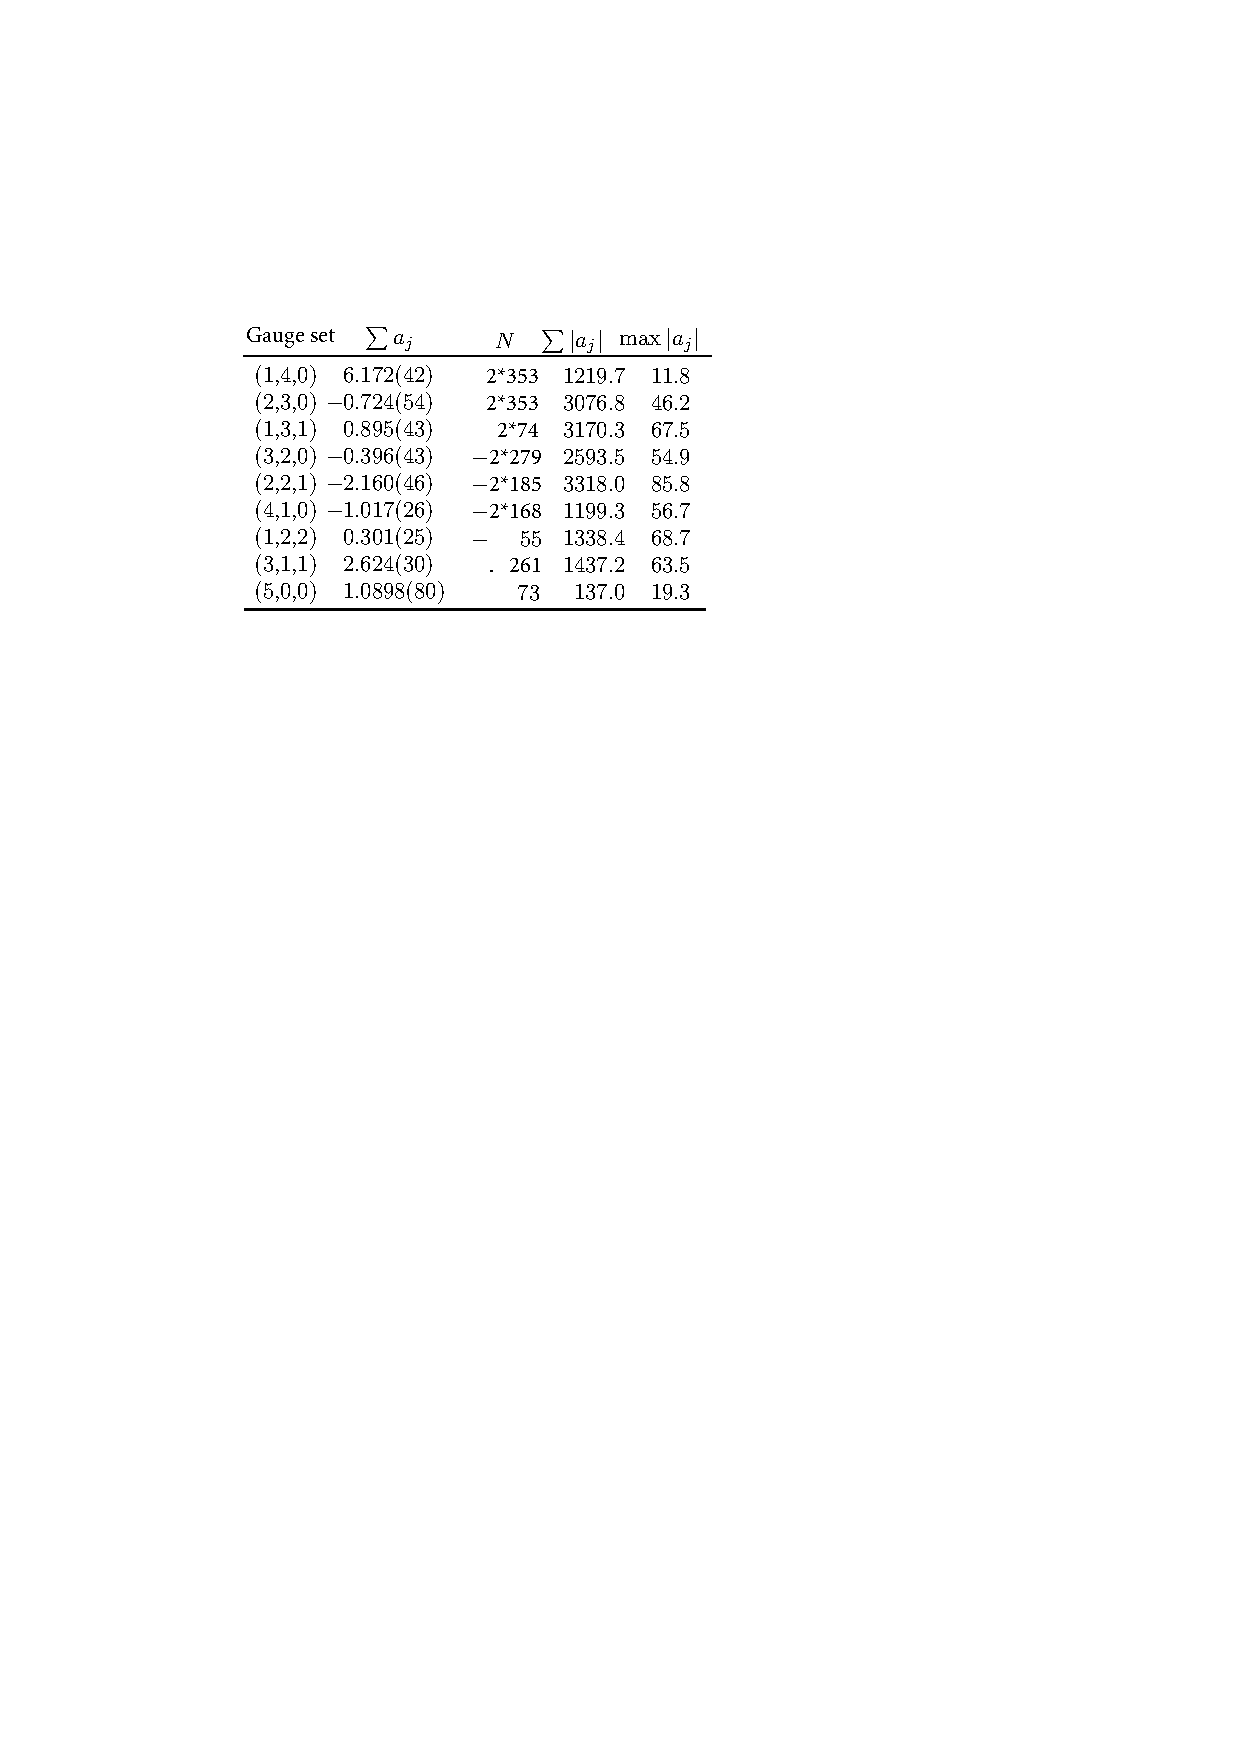
\includegraphics[width=0.60\textwidth]{Volkov19Tab1}
\end{center}
\caption{\label{Volkov19Tab1}
Contributions of the quenched QED $a^{(10)}[s]$ gauge sets, $s=(k,m,m')$.
If $m\neq m'$, the sum over $(k,m,m')+(k,m',m)$ is given, and the number
of contributing graphs is $2N_s$. Ignore the minus signs in $N$ column, a
PDF bug; I have also probably gotten the numbers of diagrams wrong.
Extracted from Volkov\rf{Volkov19} Table~1.
}
\end{table}
%%%%%%%%%%%%%%%%%%%%%%%%%%%%%%%%%%%%%%%%%%%%%%%%%%%%%%%%%%%

\item[2019-05-26 Predrag]
Volkov's
5-loop quenched QED gauge sets, are summarized in \reftab{Volkov19Tab1}.
Looking at the 4- and 5-loop results in \reftab{tabGaugeSets}, Volvkov surmises
that $(1,m,0)$ is approximately the final value, and the other values are
approximately zero with random errors (see {\bf 2018-12-21 Sergey} above).
However, gauge-set values surely do not look random to me; all signs except two
close to 0 follow my prediction, and the values are (unexplained) integers
multiples of 1/2.

Naive assumption would be that values of graphs contributing to gauge set
$s=(k,m,m')$ (do it separately from $s=(k,m',m)$ if $m\neq m'$) are uncorrelated
and randomly distributed, in which case one should test the randomness hypothesis by
computing the \emph{variance}
\beq
\expct{a^2_j}_{s} = \frac{1}{N_s}\sum_{j \in s} a^2_j
%\,.
\ee{variance_a_j}
for all gauge sets $s$ in \reftab{tabGaugeSets}, rather than listing $\sum
|a_j|$, as in Volkov's \reftab{Volkov19Tab1}, or my suggestion
\refeq{Volkov18AverMagn} above.
My interpretation of Volkov's $N_{diag}$ is likely wrong, as he writes that
``diagrams that are obtained from each other by changing arrow directions are
regarded as one,'' but that is easily fixed. It already seems that
$(5,0,0)$ and $(1,4,0)$ will be outliers.

More precisely, the {variance} is $\sigma^2=\expct{(a_j-\expct{a_j})^2}$,
and its positive square root is the \emph{standard deviation} $\sigma$.
This number depends on the gauge, and on particular auhtor's UV and IR
counter-term conventions, so it's hard to know what to make of it, but
getting a similar variance for all gauge sets would be cute.

\item[2019-06-04 Makiko Nio and Predrag to Sergey and Stefano] We have
looked together at the status of the 5-loop quenched QED, and what to do
to nail down the $4.5 \sigma$ difference between the two calculations.
Makiko's hunch is that the problem might be numerical, originating in a
Monte Carlo integral with a PDF defined in Seergey's \arXiv{1905.08007}
eq.~(1).

It looks to me that the ball is in Makiko's court; only way to compare is
via vertex diagram gauge sets, and she can do it if she really has to.

The first to check is $(5,0,0)$, both because it has the fewest diagrams,
and also because it is cleanest in terms of UV and IR counter terms. If
we ever manage to define and compute with a ``$k$-photon'' propagator,
$(k,0,0)$ has only one of them. Note also that max$|a_j|\approx 20$,
anomalously small.

$(1,4,0)$ (and the $(1,k,0)$ family of gauge sets) is fascinatingly
large. Our guess it that it might have to do with IR behaviour of the
4-loop self-energy insertion - Sergey can tell if there is something
going on there by looking at the contributing diagrams.
Note also that max$|a_j|\approx 10$, even more anomalously small, typical
size for the remaining gauge sets is max$|a_j|\approx 70$.

Next to knock off is $(1,2,2)$, then $(3,2,0)$. In my $1/2$ units I would
like to think of this set as well as $(2,2,0)$ as being approximately zero
(not to violate my gauge set sign rule).

\item[2019-09-19 Sergey] See Volkov\rf{Volkov19b} {\em }

\item[022-03-02 Sergey] See Volkov\rf{Volkov21}
{\em A way of fast calculating lepton magnetic moments in
Quantum Electrodynamics}

\item[2022-03-02 Sergey] See Volkov\rf{Volkov22}
{\em A flexible divergence elimination method for calculating
lepton magnetic moments in {Quantum Electrodynamics}}.
In principle I should check whether this is the same or different from
my methods...


\newpage
\item[2017-06-11 Predrag] to
\\
%Professor
Christian Schubert <schubert@ifm.umich.mx>
%\\
%Instituto de Física y Matem{\'a}ticas,\\
%Universidad Michoacana de San Nicol{\'a}s de Hidalgo,\\
%Ciudad Universitaria, C-3, Apdo. 2-82,\\
%C.P. 58040 Morelia, Michoacan, MEXICO
%
%\bigskip
%
%Dear Christian

Stefano Laporta  has recently published analytic values of all 4-loop
electron magnetic moment gauge sets, and they look very intriguing.
Sergey  A. Volkov has started evaluating individual 5-loop vertex
diagrams and is in position to estimate numerically the size of 5-loop
gauge sets. So it might be a good time to make a new attempt to prove/disprove
the QED finiteness conjecture. This set of notes is my current best attempt
to motivate this effort.

I do not take my 1977 ``gauge-set approximation'' very literally - its
content is only that if individual gauge sets can be bounded to anything
growing slower than combinatorially, quenched QED (and hopefully full
QED) is a finite theory, not an asymptotic series. But the form of vertex
gauge sets is very suggestive; it is defined in terms of $N$-photon
exchanges. So to me the wordline formalism seem the most promising way
forward.

While the quenched QED magnetic moment of electron is the cleanest
possible physical calculation one can do, for sociological reasons most
effort on high order estimates has gone in other directions. Do you have
a formula for spinor QED magnetic moment that one could attempt to
analyze more closely?

%As I have returned to this problem only last month, after a 40 year
%hiatus :) I would be grateful for any further pointers to the literature.

\item[2017-06-12 Christian]
I have been
fascinated by the finiteness conjecture ever after Gerald Dunne and I
were led there, too, from Euler-Heisenberg, Borel analysis,
Ritus mass shift and worldline instantons fifteen years ago.
The things have picked up a lot
just during the last year or so, namely:

\begin{enumerate}
  \item
Idrish Huet, Michel Rausch and I are working on the Affleck,
Alvarez and Manton (AAM) exponentiation conjecture\rf{AffAlMa82} in 1+1 QED.
We had a nice parameter integral representation for the three-loop
Euler-Heisenberg for quite a while, but could not get a sufficient number
of weak-field expansion coeffs out of it (so far what we got points to
AAM not holding at three loops - rather the coeffs go asymptotically
BELOW the AAM prediction - but this is very preliminary). Michel was just
visiting, and we now got a really nice algorithm (based on the polynomial
invariants of the dihedral group) for the analytical calculation of the
coeffs from the more difficult (nonplanar) 3-loop EH diagram.
  \item
If AAM really fails, then presumably the AAM worldline instanton needs
refinement at higher loops. My former student Naser Ahmadiniaz (now
postdoc in Korea) has made some progress with this.
  \item
For many years I am planning to apply the worldline formalism to (g-2),
in particular to the important graphs with the
light-by-light subdiagram. For this subdiagram I have, since a long time,
an off-shell representation that is permutation symmetric, manifestly
gauge invariant, without spurious UV poles, and moreover allows one to
trivially integrate out the one low-energy photon leg. What held me back
was that the various worldline representations that existed hitherto for
the electron line were all somewhat cumbersome, and seemed not suitable
for high-order calculations. Precisely this problem we have been working
on here for the last half year, and things have fallen into place really
nicely, we have a Bern-Kosower type master formula for the electron line
dressed with any number of photons, in vacuum and in the presence of a
constant field, and one of our students is already programming it. I am
now definitely trying to assemble a collaboration to attack the QED (g-2),
and I anticipate that your notes will be quite useful for motivating my
collaborators.

\end{enumerate}
Gies \etal\rf{GiSaVa05} have some intriguing numerical results from
worldline Monte Carlo (in section 5). Another thing I find quite
interesting are Ritus\rf{Ritus80} most recent
papers\rf{Ritus06,Ritus13,Ritus15} on the value of the bare fine
structure constant - he confirmed to me in an email from last December
(at age 90) that he definitely does not think that the bare charge is
infinite.

I am appending a summary of our efforts in this line of work\rf{HuTrSc17a}
which I wrote as a contribution to the 5th Winter Workshop on
Non-Perturbative Quantum Field Theory. 22-24 March 2017,
Sophia-Antipolis.

\item[2016-12-18 Vladimir I. Ritus] <v\_i\_ritus@mail.ru>
to Christian:

Thank you for your note about the papers by Johnson, Baker, Willey (Phys.
Rev. 1967, 1969, 1971) and by Adler, Bardeen (Phys. Rev. 1971).
    \PC{2017-08-04
    K. Johnson, M. Baker, and R. Willey, Phys. Rev. 136, B1111 (1964);
    ibid. 163, 1699 (1967); and
    S. L. Adler and W. A. Bardeen, Phys. Rev. D 4, 3045 (1971)
    These papers are about the possibility of the existence of an
    ultraviolet fixed point $\alpha_c$.
    }
I forgot them while writing my papers\rf{Ritus13,Ritus15}. Some months
ago I accidently saw  the abstracts of these papers in one of my
notebooks  with conspectus of the literature. Johnson et al assertion
confirms qualitatively my geometric and holographic duality approach to
the problem. Both of them deal with photons without self-energy
insertions. Have you any objections to this approach?

Nobody believes in infinite bare charge neither with space distribution
more singular than $\delta(x)$ nor as Landau pole at final transfer
momentum. Please, reed the several first phases in JRLR-paper (changing
the ``emitted"  to ``emitting").

I regret that I could not come to Tomsk, where I was at war time
1941-1943 in evacuation.

\item[2017-06-14 Christian to Ritus]
Just to make sure that I understand your conjecture correctly - are you
claiming that $1/4\pi$ is the value of the bare constant in the quenched
approximation, or in the full QED?

\item[2017-06-29 Vladimir Ritus]
The $1/4\pi$  is the value of the bare fine structure constant in the
full QED. It follows from duality of 4-dimensional QED and 2-dimensional
quantum field theory. The point charge moves  along timelike trajectory,
hence it has nonzero mass, but the photons emitted to infinity by this
charge are massless as the duality connected with them scalar quanta of
pairs emitted by the pointlike mirror in (1+1)-space. Constants
$\alpha_L$ and $\alpha_B$ are also geometrical. So, this theory is pure
geometrical and connected neither with the divergent perturbation theory
series, nor with the different methods of their summing. Please, read
\refrefs{Ritus13,Ritus15}.



\item[2017-06-18 Naser Ahmadiniaz] <ahmadiniaz.naser@gmail.com>
(currently a postdoctoral fellow at the Center for Relativistic Laser
Science (CoReLS), Institute for Basic Science (IBS), Gwangju, South
Korea).
\\
My main research
interests are in amplitude calculations in QED, QCD and quantum gravity
from the worldline formalism. Recently, we have been interested in
(off-shell) tree-level amplitudes for QED processes in vacuum as well as
in the presence of classical background fields which will also be applied
to higher order corrections.

\item[2017-06-20 James P. Edwards] <jedwards@ifm.umich.mx>,
%Instituto de Física y Matemáticas
%Universidad Michoacana de San Nicolás de Hidalgo
\HREF{www.ifm.umich.mx/ifm/index.php/fisca/academicos/edwards/}
{homepage}:
\\
I am currently working with Christian on the worldline approach. In some
of our recent work we have been working on more efficient ways to
determine g-2 based upon a worldline expression for the dressed spinor
propagator (both in vacuum and in a constant background).

\item[2017-06-11 Predrag] to
%\\
% Professor
Dirk Kreimer <kreimer@physik.hu-berlin.de>
%\\
%Humboldt-Universit\"at zu Berlin\\
%Institut f\"r Mathematik\\
%\bigskip
%
%Dear Dirk
%
%\medskip

Stefano Laporta  has recently published analytic values of all 4-loop
electron magnetic moment gauge sets, and they look very intriguing.
It might be a good time to make a new attempt to prove/disprove
the QED finiteness conjecture. This set of notes is my current best attempt
to motivate this effort.

If individual gauge sets can be bounded to anything growing slower than
combinatorially, quenched QED (and hopefully full QED) is a finite
theory, not an asymptotic series. The form of vertex gauge sets is
suggestive of a way forward; it is defined in terms of $N$-photon
exchanges. Hopf algebras might hold the key, but I do not know how to use
these ideas.

I would be grateful for any further pointers to the literature.
Anybody else I should send these notes to? And I'm
finally ready to stand up an be counted - I can fly to Berlin on a short
notice if that helps.

%\bigskip
%
%\noindent
%best regards
%\\
%Predrag
%\newpage

\item[2017-06-14 Dirk Kreimer] was kind enough to invite me to
\HREF{http://www2.mathematik.hu-berlin.de/~kreimer/wp-content/uploads/houches2018.html}
{Les Houches — June 4-15, 2018} on structures in local quantum field
theory. Edwards and I went, and learned a whole lot.

\item[2019-06-03 Christian Schubert and James P. Edwards]
We are still making sense of our master formulae but things are falling
into place. Our worldline efforts still are not paying off - a whole
class of terms that we had thought would not contribute on-shell for the
open fermion line actually does, And there is still the question whether
$g-2$ should be calculated in x-space or in p-space on the worldline
$\dots$ . We will keep you updated.

\item[2020-06-04 Somdatta Bhattacharya] <somdatta.bhattacharya@gmail.com>
writes: ``
I am intrigued by something you're an expert on. Soft photons correct the
QED vertex, so why don't they also affect $F_2(0)$ by a finite amount?
''
\\
{\bf Predrag} Dear Somdatta, \emph{you} are the expert\rf{Bhattacharya17}
:) Soft photons (were there an unambiguous gauge-invariant definition
that included both the IR divergences and the finite parts) contribute to
all radiative QED corrections, so surely they contribute to $g-2$
anomaly.

Here is my 5 cents. It's hand-waving, so I only say it in the privacy
of my QFT class - if you can turn it into mathematics, I would be grateful.

For me the IR and UV divergences exist on the same footing, even
cancelling each other\rf{MassShell}. However, the anomaly
\refeq{IRstruct(1)Q} does not have either\rf{IRstruct}. Why?

$F_2(0)$ part of the QED vertex form factor corresponds to flipping
the electron spin; soft photon cannot do that, that's why there is no
IR divergence. When you look at the parametric form of the
integral for $a_{0}^{(2)}$ it looks like the dominant contribution
is halfway where the infrared and ultraviolet singularities
would have been. So in my book, the soft photons are about 50\%
of the $F_2(0)$ anomaly.

PS If you actually read {\em Infra-red structure of {Yang-Mills}
theories}\rf{IRstruct}, it is not a stupid paper. That's why is has
garnered the total of 14 citations. I would be grateful for any earlier
(or later) reference that does it better or explains it more clearly.

PPS Maybe I should read
Fleischer and Tarasov\rf{FleTar92}
{\em Gauge-invariant on-shell {$Z_1$} in {QED} and {QCD}}?
(I do not have access to it online)

\item[2020-06-04 Somdatta Bhattacharya]
Here's my argument for why the $F_2(0)$ is zero at least up to first order,
but I end with a conundrum.

The amplitude for the vertex with the soft photon is akin to the Compton
scattering amplitude, with one of the photons being the soft one and the
other being the one of the vertex. In the limit of small photon momenta,
it is proportional to
$\overline{u}(p'.e/p'.k - p.e/p.k)\gamma^mu$
sandwiched
between the electron spinor states, where p' and p are the electron
momenta and k is the soft-photon one, e being the soft photon
polarization.

In the usual analysis, when you sum over polarizations and integrate for
the invariant momentum measure for k over the square of the expression
you get the Sudakov double logs in the scattering amplitude, that cancel
a similar expression coming from the loops, that is the $F_1$. I am
following Peskin and Schroeder.

Notice that the expression for the soft photons is exact, so that is all
that is there to it, and hence it doesn't give any contribution to
$F_2(0)$.

However, here's something interesting.

You get $(p'.e/p'.k-p.e/p.k)$ by acting with the Dirac operators on
specific spinors on either side of the Compton amplitude. But what if you
exchange p' and p by using momentum conservation and make the
corresponding Dirac operators act on the spinors on opposite sides. You
would get a totally different expression, involving
$[(p'.)/p'.k-(p.)/p.k](\gamma.e)$.
Now, ``in principle" such an expression ought to be
re-expressible in terms of
\(
\sigma. q.e. (F_2(p,p',k)) + \gamma.e(F_1(p,p',k))
\)
for some $F_2$ and $F_1$. The dots in the subscripts stand for greek
indices in the sigma expression.

And when squared and integrated over would give rise to a Rosenbluth-like
formula for electron scattering when one does the integral over k, from
which one can extract the ``effective" F's. Then setting the q to zero,
one should get the $F_2(0)$. Notice that like the $F_1$, this too would be
possibly divergent.

The only trouble is the finite q expressions should match with the result
computed using $(p'.e/p'.k - p.e/p.k)$, which gives just an $F_1$. But
this can't be possible, but I can't figure out the mistake in the naive
analysis. This is the conundrum I was referring to.

This is all I have come up with till now.

Here's something you might find of interest: \\
\emph{alternative worldline new.pdf} ;\;
\emph{SM from GR.pdf} \,.

Here's a rough draft I have written on new ways of doing QED one-loop calculations and their advantages. It's meant to open up discussions/collaboration:
\emph{QED new.pdf}.
Please take a look and let me know what you feel.

\item[2022-12-30 Christian Schubert]
Vladimir Ritus seems to be very anxious to have your opinion on
his papers about the calculation of alpha.

\end{description}
